\chapter{民數記}

\section{在西乃的末期 1-10}

\subsection{數點以色列人，各支派依序安營 1:1－2:31}
\subsubsection{核以色列族能臨陣男丁之總數 1:1-3}
以色列人出埃及地後，第二年二月初一日，耶和華在西奈的曠野，會幕中曉諭摩西說：「你要按以色列全會眾的家室、宗族，人名的數目，計算所有的男丁。凡以色列中，從二十歲以外，能出去打仗的，你和亞倫要照他們的軍隊數點。

\subsubsection{派定各族族長 1:4-19}
每支派中，必有一人做本支派的族長，幫助你們。他們的名字：屬\textcolor{blue}{魯本}的，有示丟珥的兒子以利蓿；屬\textcolor{blue}{西緬}的，有蘇利沙代的兒子示路蔑；屬\textcolor{blue}{猶大}的，有亞米拿達的兒子拿順；屬\textcolor{blue}{以薩迦}的，有蘇押的兒子拿坦業；屬\textcolor{blue}{西布倫}的，有希倫的兒子以利押；\textcolor{blue}{約瑟}子孫屬\textcolor{blue}{以法蓮}的，有亞米忽的兒子以利沙瑪；屬\textcolor{blue}{瑪拿西}的，有比大蓿的兒子迦瑪列；屬\textcolor{blue}{便雅憫}的，有基多尼的兒子亞比但；屬\textcolor{blue}{但}的，有亞米沙代的兒子亞希以謝； 屬\textcolor{blue}{亞設}的，有俄蘭的兒子帕結；屬\textcolor{blue}{迦得}的，有丟珥的兒子以利雅薩；屬\textcolor{blue}{拿弗他利}的，有以南的兒子亞希拉。這都是從會中選召的，各做本支派的首領，都是以色列軍中的統領。」於是摩西、亞倫帶著這些按名指定的人，當二月初一日招聚全會眾。會眾就照他們的家室、宗族，人名的數目，從二十歲以外的，都述說自己的家譜。耶和華怎樣吩咐摩西，他就怎樣在西奈的曠野數點他們。

\subsubsection{以色列族被统计的男丁總數 1:20-46}
\begin{wraptable}{r}{10.cm}
\vspace*{-8mm}
\centering
\begin{tabular}{c|c|c|c|c|c}\hline\hline
支派  & 首領名字&  父親名字 &第一次&第二次 &增减\\\hline
流便  &以利蓿 & 示丟珥&46,500 & &\\
西緬  & 示路蔑 &  蘇利沙代&59,300 & & \\
猶大 & 拿順 &亞米拿達&74,600 & &\\
以薩迦 &拿坦業  & 蘇押&54,400 & & \\
西布倫&  以利押& 希倫&57,400 & & \\
以法蓮  &以利沙瑪 & 亞米忽&40,500 & &\\
瑪拿西  & 迦瑪列 &  比大蓿&32,200 & & \\
便雅憫 &亞比但 &基多尼&35,400 && \\
但  &亞希以謝 & 亞米沙代&62,700 && \\
亞設  & 帕結 &  俄蘭&41,500 & & \\
迦得&以利雅薩 & 丟珥&45,650 & & \\
拿弗他利&亞希拉 & 以南&53,400 & & \\\hline
總數&&&603,550&&\\\hline
\end{tabular}
\caption{以色列族被统计的男丁總數}
\end{wraptable}
以色列的長子魯本子孫的後代，照著家室、宗族，人名的數目，從二十歲以外，凡能出去打仗，被數的男丁共有四萬六千五百名。西緬子孫的後代，照著家室、宗族，人名的數目，從二十歲以外，凡能出去打仗，被數的男丁共有五萬九千三百名。迦得子孫的後代，照著家室、宗族，人名的數目，從二十歲以外，凡能出去打仗，被數的共有四萬五千六百五十名。猶大子孫的後代，照著家室、宗族，人名的數目，從二十歲以外，凡能出去打仗，被數的共有七萬四千六百名。以薩迦子孫的後代，照著家室、宗族，人名的數目，從二十歲以外，凡能出去打仗，被數的共有五萬四千四百名。西布倫子孫的後代，照著家室、宗族，人名的數目，從二十歲以外，凡能出去打仗，被數的共有五萬七千四百名。約瑟子孫，屬以法蓮子孫的後代，照著家室、宗族，人名的數目，從二十歲以外，凡能出去打仗，被數的共有四萬零五百名。 瑪拿西子孫的後代，照著家室、宗族，人名的數目，從二十歲以外，凡能出去打仗，被數的共有三萬二千二百名。便雅憫子孫的後代，照著家室、宗族，人名的數目，從二十歲以外，凡能出去打仗，被數的共有三萬五千四百名。但子孫的後代，照著家室、宗族，人名的數目，從二十歲以外，凡能出去打仗，被數的共有六萬二千七百名。亞設子孫的後代，照著家室、宗族，人名的數目，從二十歲以外，凡能出去打仗，被數的共有四萬一千五百名。拿弗他利子孫的後代，照著家室、宗族，人名的數目，從二十歲以外，凡能出去打仗，被數的共有五萬三千四百名。這些就是被數點的，是摩西、亞倫和以色列中十二個首領所數點的，這十二個人各做各宗族的代表。這樣，凡以色列人中被數的，照著宗族從二十歲以外，能出去打仗，被數的共有六十萬零三千五百五十名。

\subsubsection{利未支派不列其數 1:47-54}
利未人卻沒有按著支派數在其中， 48 因為耶和華曉諭摩西說： 49 「唯獨利未支派你不可數點，也不可在以色列人中計算他們的總數。 50 只要派利未人管法櫃的帳幕和其中的器具，並屬乎帳幕的。他們要抬(搬運)帳幕和其中的器具，並要辦理帳幕的事，在帳幕的四圍安營。 51 帳幕將往前行的時候，利未人要拆卸；將支搭的時候，利未人要豎起。近前來的外人必被治死。 52 以色列人支搭帳篷，要照他們的軍隊，各歸本營，各歸本纛。 53 但利未人要在法櫃帳幕的四圍安營，免得憤怒臨到以色列會眾。利未人並要謹守法櫃的帳幕。」 54 以色列人就這樣行。凡耶和華所吩咐摩西的，他們就照樣行了。


\subsubsection{東邊支派首領及安營之所 2:1-8}
\begin{wrapfigure}{r}{0.5\textwidth}
\vspace*{-22mm}
\begin{center} 
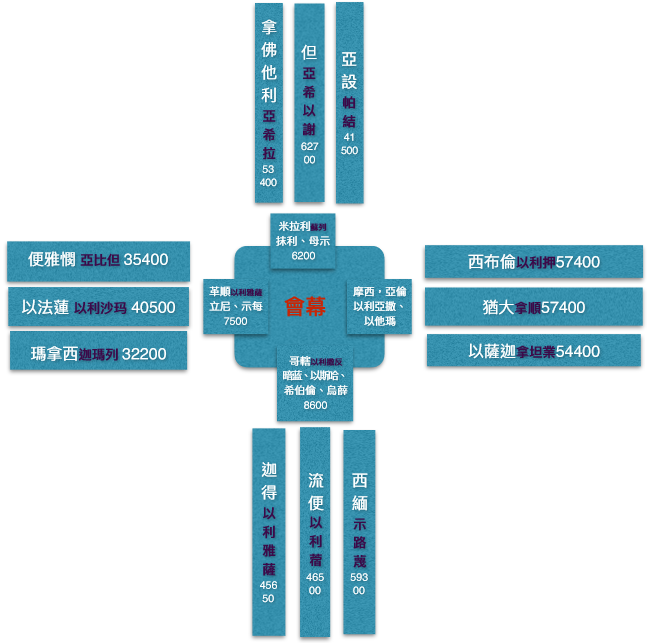
\includegraphics[width=0.85\textwidth]{AMoXiFigs/fig1}
\caption{各支派族長，人數及位置}
\label{fig:1} 
\end{center}
\end{wrapfigure}
耶和華曉諭摩西、亞倫說：「以色列人要各歸自己的纛下，在本族的旗號那裡，對著會幕的四圍安營。在\textcolor{red}{東邊}向日出之地，照著軍隊安營的是猶大營的纛。有亞米拿達的兒子拿順做猶大人的首領， 4 他軍隊被數的，共有七萬四千六百名； 5 挨著他安營的是以薩迦支派，有蘇押的兒子拿坦業做以薩迦人的首領， 6 他軍隊被數的，共有五萬四千四百名； 7 又有西布倫支派，希倫的兒子以利押做西布倫人的首領， 8 他軍隊被數的，共有五萬七千四百名。 9 凡屬猶大營，按著軍隊被數的，共有十八萬六千四百名，要做第一隊往前行。

\subsubsection{南邊支派首領及安營之所 2:9-16}
在\textcolor{red}{南邊}，按著軍隊是魯本營的纛。有示丟珥的兒子以利蓿做魯本人的首領， 11 他軍隊被數的，共有四萬六千五百名； 12 挨著他安營的是西緬支派，蘇利沙代的兒子示路蔑做西緬人的首領， 13 他軍隊被數的，共有五萬九千三百名； 14 又有迦得支派，丟珥的兒子以利雅薩做迦得人的首領， 15 他軍隊被數的，共有四萬五千六百五十名。 16 凡屬魯本營，按著軍隊被數的，共有十五萬一千四百五十名，要做第二隊往前行。

\subsubsection{利未營在諸營中間 2:17}
隨後會幕要往前行，有利未營在諸營\textcolor{red}{中間}。他們怎樣安營就怎樣往前行，各按本位，各歸本纛。

\subsubsection{西邊支派首領及安營之所 2:18-24}
在\textcolor{red}{西邊}，按著軍隊是以法蓮營的纛。亞米忽的兒子以利沙瑪做以法蓮人的首領， 19 他軍隊被數的，共有四萬零五百名； 20 挨著他的是瑪拿西支派，比大蓿的兒子迦瑪列做瑪拿西人的首領， 21 他軍隊被數的，共有三萬二千二百名； 22 又有便雅憫支派，基多尼的兒子亞比但做便雅憫人的首領， 23 他軍隊被數的，共有三萬五千四百名。 24 凡屬以法蓮營，按著軍隊被數的，共有十萬零八千一百名，要做第三隊往前行。

\subsubsection{北邊支派首領及安營之所 2:25-31}
在\textcolor{red}{北邊}，按著軍隊是但營的纛。亞米沙代的兒子亞希以謝做但人的首領， 26 他軍隊被數的，共有六萬二千七百名； 27 挨著他安營的是亞設支派，俄蘭的兒子帕結做亞設人的首領， 28 他軍隊被數的，共有四萬一千五百名； 29 又有拿弗他利支派，以南的兒子亞希拉做拿弗他利人的首領， 30 他軍隊被數的，共有五萬三千四百名。 31 凡但營被數的，共有十五萬七千六百名，要歸本纛做末隊往前行。

\subsection{數點利未支派 2:32－4:49}
\subsubsection{唯獨利未人沒有被數 2:32-34}
這些以色列人，照他們的宗族，按他們的軍隊，在諸營中被數的，共有六十萬零三千五百五十名。唯獨利未人沒有數在以色列人中，是照耶和華所吩咐摩西的。以色列人就這樣行，各人照他們的家室、宗族歸於本纛，安營起行，都是照耶和華所吩咐摩西的。

\subsubsection{亞倫和摩西的後代 3:1-4}
\begin{wraptable}{r}{5.cm}
\vspace*{-5mm}
\centering
\begin{tabular}{ c|c|c }\hline\hline
拿答-長子 & 獻凡火而死&受膏祭司\\ 
亞比戶 &獻凡火而死&受膏祭司\\  
以利亞撒 &供祭司職分&受膏祭司   \\
以他瑪  & 供祭司職分&受膏祭司   \\\hline
\end{tabular}
\caption{亞倫後裔}
\end{wraptable}
耶和華在西奈山曉諭摩西的日子，亞倫和摩西的後代如下：亞倫的兒子，長子名叫拿答，還有亞比戶、以利亞撒、以他瑪。這是亞倫兒子的名字，都是受膏的祭司，是摩西叫他們承接聖職供祭司職分的。拿答、亞比戶在西奈的曠野向耶和華獻凡火的時候，就死在耶和華面前了，他們也沒有兒子。以利亞撒、以他瑪在他們的父親亞倫面前供祭司的職分。

\subsubsection{區別利未人服侍亞倫 3:5-10}

耶和華曉諭摩西說：「你使利未支派近前來，站在祭司亞倫面前好服侍他，替他和會眾在會幕前守所吩咐的，辦理帳幕的事。又要看守會幕的器具，並守所吩咐以色列人的，辦理帳幕的事。你要將利未人給亞倫和他的兒子，因為他們是從以色列人中選出來給他的。你要囑咐亞倫和他的兒子謹守自己祭司的職任。近前來的外人必被治死。」

\subsubsection{利未人代替以色列人一切頭生 3:11-13}
耶和華曉諭摩西說： 12 「我從以色列人中揀選了利未人，代替以色列人一切頭生的，利未人要歸我， 13 因為凡頭生的是我的。我在埃及地擊殺一切頭生的那日，就把以色列中一切頭生的，連人帶牲畜都分別為聖歸我，他們定要屬我。我是耶和華。」

\subsubsection{利未宗族的家室 3:14-20}
\begin{figure}[H]
\centering
%\begin{center}
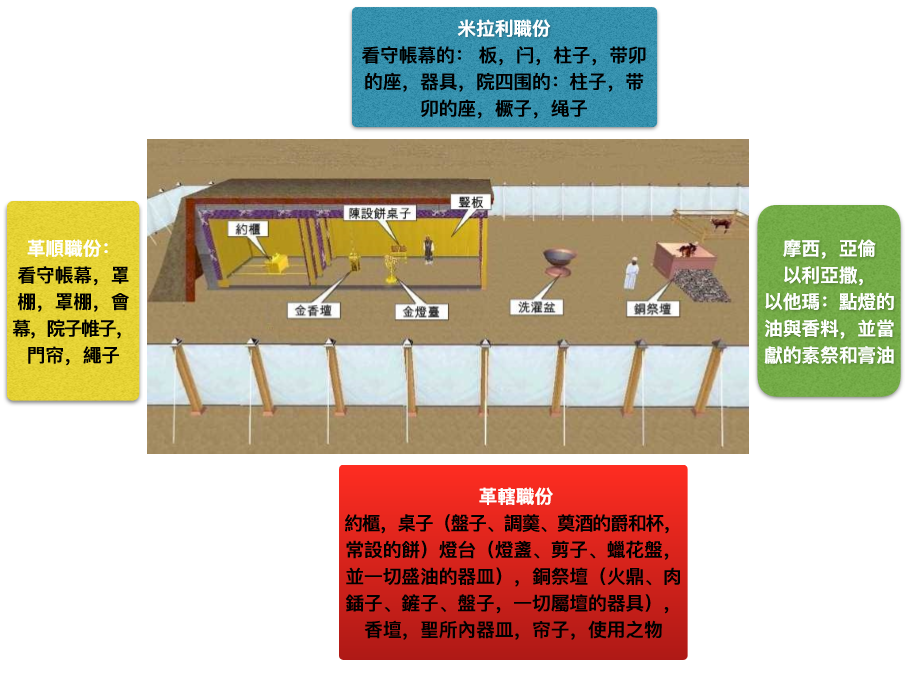
\includegraphics[width=5in]{AMoXiFigs/fig2}
\caption{圖2：利未各支派職分及位置}
\label{fig:1} 
%\end{center}
\end{figure}
耶和華在西奈的曠野曉諭摩西說： 15 「你要照利未人的宗族、家室數點他們，凡一個月以外的男子都要數點。」 16 於是摩西照耶和華所吩咐的，數點他們。 17 利未眾子的名字是革順、哥轄、米拉利。 18 革順的兒子，按著家室，是立尼、示每； 19 哥轄的兒子，按著家室，是暗蘭、以斯哈、希伯倫、烏薛； 20 米拉利的兒子，按著家室，是抹利、母示。這些按著宗族是利未人的家室。

\subsubsection{革順男丁之數及職份 3:21-26}
屬革順的，有立尼族、示每族，這是革順的二族。其中被數，從一個月以外所有的男子，共有七千五百名。這革順的二族要在帳幕後西邊安營。拉伊勒的兒子以利雅薩做革順人宗族的首領。革順的子孫在會幕中所要看守的，就是帳幕和罩篷，並罩篷的蓋與會幕的門簾，院子的帷子和門簾（院子是圍帳幕和壇的），並一切使用的繩子。

\subsubsection{革轄男丁之數及職份 3:27-43}
屬哥轄的，有暗蘭族、以斯哈族、希伯倫族、烏薛族，這是哥轄的諸族。按所有男子的數目，從一個月以外看守聖所的，共有八千六百名。哥轄兒子的諸族要在帳幕的南邊安營。烏薛的兒子以利撒反做哥轄宗族家室的首領。他們所要看守的是約櫃、桌子、燈臺、兩座壇與聖所內使用的器皿，並簾子和一切使用之物。祭司亞倫的兒子以利亞撒做利未人眾首領的領袖，要監察那些看守聖所的人。

\subsubsection{米拉利男丁之數及職份 3:33-37}
屬米拉利的，有瑪利族、母示族，這是米拉利的二族。他們被數的，按所有男子的數目，從一個月以外的，共有六千二百名。亞比亥的兒子蘇列做米拉利二宗族的首領。他們要在帳幕的北邊安營。米拉利子孫的職分是看守帳幕的板、閂、柱子、帶卯的座和帳幕一切所使用的器具，院子四圍的柱子、帶卯的座、橛子和繩子。

\subsubsection{摩西、亞倫和亞倫兒子的職份 3:38}
在帳幕前東邊向日出之地安營的是摩西、亞倫和亞倫的兒子。他們看守聖所，替以色列人守耶和華所吩咐的。近前來的外人必被治死。 

\subsubsection{利未人代替以色列族首生之男 3:39-51}
\begin{table}[H]
\centering
\begin{tabular}{c|c|c|c|c}
\hline
\hline
    &革順  & 革轄  & 米拉利&  總數  \\
\hline
各族     & 立尼，示每 & 暗蘭，以斯哈，希伯倫，烏薛  & 抹利，母示&   \\
\hline
人數（一個月以上）&7500&8600&6200&22000  \\ 
\hline
人數（30-50歲）& 2630 &  2750 &3200&8580  \\
\hline
\end{tabular}
\caption{利未支派}
\end{table}
39 凡被數的利未人，就是摩西、亞倫照耶和華吩咐所數的，按著家室，從一個月以外的男子，共有二萬二千名。

40 耶和華對摩西說：「你要從以色列人中數點一個月以外，凡頭生的男子，把他們的名字記下。 41 我是耶和華。你要揀選利未人歸我，代替以色列人所有頭生的；也取利未人的牲畜，代替以色列所有頭生的牲畜。」 42 摩西就照耶和華所吩咐的，把以色列人頭生的都數點了。 43 按人名的數目，從一個月以外，凡頭生的男子，共有二萬二千二百七十三名。

 耶和華曉諭摩西說：「你揀選利未人代替以色列人所有頭生的，也取利未人的牲畜代替以色列人的牲畜。利未人要歸我。我是耶和華。以色列人中頭生的男子比利未人多二百七十三個，必當將他們贖出來。你要按人丁，照聖所的平，每人取贖銀五舍客勒（一舍客勒是二十季拉），把那多餘之人的贖銀交給亞倫和他的兒子。」於是摩西從那被利未人所贖以外的人取了贖銀。從以色列人頭生的所取之銀，按聖所的平，有一千三百六十五舍客勒。摩西照耶和華的話把這贖銀給亞倫和他的兒子，正如耶和華所吩咐的。

\subsubsection{祭司亞倫和兒子職任 4:1-14}
耶和華曉諭摩西、亞倫說：「你從利未人中，將哥轄子孫的總數，照他們的家室、宗族，從三十歲直到五十歲，凡前來任職，在會幕裡辦事的，全都計算。哥轄子孫在會幕搬運至聖之物，所辦的事乃是這樣：起營的時候，亞倫和他兒子要進去
\begin{itemize} 
\itemsep-.35em
\item 摘下遮掩櫃的幔子，用以蒙蓋\textcolor{blue}{法櫃}。又用海狗皮蓋在上頭，再蒙上純藍色的毯子，把\textcolor{red}{槓}穿上。
\item 又用藍色毯子鋪在\textcolor{blue}{陳設餅的桌子上}，將盤子、調羹、奠酒的爵和杯擺在上頭，桌子上也必有常設的餅。在其上又要蒙朱紅色的毯子，再蒙上海狗皮，把\textcolor{red}{槓}穿上。
\item 要拿藍色毯子，把\textcolor{blue}{燈臺和燈臺上所用的}燈盞、剪子、蠟花盤並一切盛油的器皿，全都遮蓋。又要把燈臺和燈臺的一切器具包在海狗皮裡，放在\textcolor{red}{抬架}上。
\item 在\textcolor{blue}{金壇}上要鋪藍色毯子，蒙上海狗皮，把\textcolor{red}{槓}穿上。
\item 又要把聖所用的\textcolor{blue}{一切器具}包在藍色毯子裡，用海狗皮蒙上，放在\textcolor{red}{抬架}上。
\item 要收去壇上的灰，把紫色毯子鋪在壇上。又要把所用的一切器具，就是火鼎、肉叉子、鏟子、盤子，一切\textcolor{blue}{屬壇的器具}都擺在壇上。又蒙上海狗皮，把\textcolor{red}{槓}穿上。 
\end{itemize}

\subsubsection{哥轄子孫之職任 4:15-20}
將要起營的時候，\textcolor{blue}{亞倫和他兒子}把聖所和聖所的一切器具遮蓋完了，\textcolor{blue}{哥轄的子孫}就要來抬，只是不可摸聖物，免得他們死亡。會幕裡這些物件是哥轄子孫所當抬的。\textcolor{blue}{祭司亞倫的兒子以利亞撒}所要看守的是點燈的油與香料，並當獻的素祭和膏油，也要看守全帳幕與其中所有的，並聖所和聖所的器具。
耶和華曉諭摩西、亞倫說：「你們不可將哥轄人的支派從利未人中剪除。他們挨近至聖物的時候，\textcolor{blue}{亞倫和他兒子}要進去，派他們各人所當辦的、所當抬的。這樣待他們，好使他們活著，不致死亡。只是他們連片時不可進去觀看聖所，免得他們死亡。」

\subsubsection{革順子孫在以他瑪手下之職任 4:21-28}
耶和華曉諭摩西說：「你要將革順子孫的總數，照著宗族、家室，從三十歲直到五十歲，凡前來任職，在會幕裡辦事的，全都數點。革順人各族所辦的事、所抬的物乃是這樣：他們要抬帳幕的\textcolor{blue}{幔子}和會幕，並會幕的\textcolor{blue}{蓋}與其上的\textcolor{blue}{海狗皮}和會幕的\textcolor{blue}{門簾}，院子的\textcolor{blue}{帷子}和\textcolor{blue}{門簾}（院子是圍帳幕和壇的）、\textcolor{blue}{繩子}，並所用的\textcolor{blue}{器具}，不論是做什麼用的，他們都要經理。革順的子孫在一切抬物辦事之上都要憑亞倫和他兒子的吩咐。他們所當抬的，要派他們看守。這是革順子孫的各族在會幕裡所辦的事。他們所看守的，必在祭司亞倫兒子以他瑪的手下。

\subsubsection{米拉利子孫在以他瑪手下之職任 4:29-33}
至於米拉利的子孫，你要照著家室、宗族把他們數點。從三十歲直到五十歲，凡前來任職，在會幕裡辦事的，你都要數點。他們辦理會幕的事，就是抬帳幕的\textcolor{blue}{板、閂、柱子和帶卯的座}，院子四圍的\textcolor{blue}{柱子}和其上\textcolor{blue}{帶卯的座}，\textcolor{blue}{橛子}、\textcolor{blue}{繩子}，並\textcolor{blue}{一切使用的器具}。他們所抬的器具，你們要按名指定。這是米拉利子孫各族在會幕裡所辦的事，都在祭司亞倫兒子以他瑪的手下。

\subsubsection{記利未人自三十歲至五十歲者之數 4:34-49}
摩西、亞倫與會眾的諸首領將\textcolor{blue}{哥轄的子孫}，照著家室、宗族，從三十歲直到五十歲，凡前來任職，在會幕裡辦事的，都數點了，被數的共有二千七百五十名。這是哥轄各族中被數的，是在會幕裡辦事的，就是摩西、亞倫照耶和華藉摩西所吩咐數點的。
\textcolor{blue}{革順子孫}被數的，照著家室、宗族，從三十歲直到五十歲，凡前來任職，在會幕裡辦事的，共有二千六百三十名。這是革順子孫各族中被數的，是在會幕裡辦事的，就是摩西、亞倫照耶和華藉摩西所吩咐數點的。
\textcolor{blue}{米拉利子孫}中各族被數的，照著家室、宗族， 從三十歲直到五十歲，凡前來任職，在會幕裡辦事的，共有三千二百名。 這是米拉利子孫各族中被數的，就是摩西、亞倫照耶和華藉摩西所吩咐數點的。
凡\textcolor{blue}{被數的利未人}，就是摩西、亞倫並以色列眾首領，照著家室、宗族所數點的，從三十歲直到五十歲，凡前來任職，在會幕裡做抬物之工的，共有八千五百八十名。摩西按他們所辦的事、所抬的物，憑耶和華的吩咐數點他們。他們這樣被摩西數點，正如耶和華所吩咐他的。


\subsection{頒布生活，婚姻，生命潔净的律法 5-6}
\subsubsection{不潔者出到營外 5:1-4 }
耶和華曉諭摩西說：「你吩咐以色列人，使一切長大痲瘋的、患漏症的並因死屍不潔淨的，都出營外去。無論男女都要使他們出到營外，免得汙穢他們的營。這營是我所住的。」以色列人就這樣行，使他們出到營外。耶和華怎樣吩咐摩西，以色列人就怎樣行了。

\subsubsection{犯罪的要賠償 5:5-8}
耶和華對摩西說：「你曉諭以色列人說：無論男女，若犯了人所常犯的罪，以致干犯耶和華，那人就有了罪。他要承認所犯的罪，將所虧負人的如數賠還，另外加上五分之一，也歸於所虧負的人。那人若沒有親屬可受所賠還的，那所賠還的就要歸於服侍耶和華的祭司。至於那為他贖罪的公羊是在外。以色列人一切的聖物中，所奉給祭司的舉祭都要歸於祭司。各人所分別為聖的物，無論是什麼，都要歸給祭司。」

\subsubsection{歸給祭司的物 5:9-10}
以色列人一切的聖物中，所奉給祭司的舉祭都要歸於祭司。各人所分別為聖的物，無論是什麼，都要歸給祭司。

\subsubsection{妻子貞節實驗方法 5:11-31}
耶和華對摩西說： 12 「你曉諭以色列人說：人的妻若有邪行，得罪她丈夫， 13 有人與她行淫，事情嚴密，瞞過她丈夫，而且她被玷汙，沒有做見證的人，當她行淫的時候也沒有被捉住， 14 她丈夫生了疑恨的心，疑恨她，她是被玷汙，或是她丈夫生了疑恨的心，疑恨她，她並沒有被玷汙， 15 這人就要將妻送到祭司那裡，又為她帶著大麥麵伊法十分之一做供物，不可澆上油，也不可加上乳香，因為這是疑恨的素祭，是思念的素祭，使人思念罪孽。

祭司要使那婦人近前來，站在耶和華面前。 17 祭司要把聖水盛在瓦器裡，又從帳幕的地上取點塵土，放在水中。 18 祭司要叫那婦人蓬頭散髮，站在耶和華面前，把思念的素祭，就是疑恨的素祭，放在她手中。祭司手裡拿著致咒詛的苦水， 19 要叫婦人起誓，對她說：『若沒有人與你行淫，也未曾背著丈夫做汙穢的事，你就免受這致咒詛苦水的災。 20 你若背著丈夫行了汙穢的事，在你丈夫以外有人與你行淫， 21 （祭司叫婦人發咒起誓）願耶和華叫你大腿消瘦，肚腹發脹，使你在你民中被人咒詛，成了誓語， 22 並且這致咒詛的水入你的腸中，要叫你的肚腹發脹，大腿消瘦。』婦人要回答說：『阿們！阿們！』

祭司要寫這咒詛的話，將所寫的字抹在苦水裡， 24 又叫婦人喝這致咒詛的苦水。這水要進入她裡面變苦了。 25 祭司要從婦人的手中取那疑恨的素祭，在耶和華面前搖一搖，拿到壇前。 26 又要從素祭中取出一把，作為這事的紀念，燒在壇上，然後叫婦人喝這水。 27 叫她喝了以後，她若被玷汙，得罪了丈夫，這致咒詛的水必進入她裡面變苦了，她的肚腹就要發脹，大腿就要消瘦，那婦人便要在她民中被人咒詛； 28 若婦人沒有被玷汙，卻是清潔的，就要免受這災，且要懷孕。

妻子背著丈夫行了汙穢的事， 30 或是人生了疑恨的心，疑恨他的妻，就有這疑恨的條例。那時他要叫婦人站在耶和華面前，祭司要在她身上照這條例而行。 31 男人就為無罪，婦人必擔當自己的罪孽。

\noindent
疑恨（思念）的素祭=大麥麵1/10伊法+無油無乳香\\
1） 過程\\
  祭司要使那婦人近前來，站在耶和華面前發咒起誓；
  婦人要回答說：『阿們，阿們。』
  祭司要寫這咒詛的話，將所寫的字抹在苦水裏，從素祭中取出一把燒在壇上，叫婦人喝這水\\
2）判斷方法 \\
   $\cdot${ 她若被玷污得罪了丈夫，這致咒詛的水必進入她裏面變變苦了，她的肚腹就要發脹，大腿就要消瘦，那婦人便要在他民中被人咒詛。}\\
   $\cdot${ 若婦人沒有被玷污，卻是清潔的，就要免受這災，且要懷孕。}


\subsubsection{拿細耳人的條例 6:1-21}
\subsubsubsection{做拿細耳(歸主)人的要求 6:1-8}
耶和華對摩西說：「你曉諭以色列人說：無論男女許了特別的願，就是拿細耳(歸主)人的願，要離俗歸耶和華，
\vspace*{-2mm}
\begin{itemize} 
\itemsep-.35em
\item 他就要遠離清酒濃酒，也不可喝什麼清酒濃酒做的醋。不可喝什麼葡萄汁，也不可吃鮮葡萄和乾葡萄。在一切離俗的日子，凡葡萄樹上結的，自核至皮所做的物，都不可吃。
\item 在他一切許願離俗的日子，不可用剃頭刀剃頭，要由髮綹長長了。他要聖潔，直到離俗歸耶和華的日子滿了。
\item 在他離俗歸耶和華的一切日子，不可挨近死屍。他的父母或是弟兄姐妹死了的時候，他不可因他們使自己不潔淨，因為那離俗歸神的憑據是在他頭上。在他一切離俗的日子，是歸耶和華為聖。
\end{itemize} 

\subsubsubsection{拿細耳(歸主)人被沾染的要求 6:9-12}
\begin{itemize} 
\itemsep-.35em
\item 若在他旁邊忽然有人死了，以致沾染了他離俗的頭，他要在第七日得潔淨的時候剃頭。第八日，他要把兩隻斑鳩或兩隻雛鴿帶到會幕門口，交給祭司。
\item 祭司要獻一隻做贖罪祭，一隻做燔祭，為他贖那因死屍而有的罪，並要當日使他的頭成為聖潔。
\item 他要另選離俗歸耶和華的日子，又要牽一隻一歲的公羊羔來做贖愆祭；但先前的日子要歸徒然，因為他在離俗之間被玷汙了。
\end{itemize} 

\subsubsubsection{拿細耳(歸主)滿了離俗期的條例 6:13-21}
拿細耳人滿了離俗的日子乃有這條例：
\vspace*{-2mm}
\begin{itemize} 
\itemsep-.35em
\item 人要領他到會幕門口，他要將供物奉給耶和華，就是一隻沒有殘疾、一歲的公羊羔做燔祭，一隻沒有殘疾、一歲的母羊羔做贖罪祭，和一隻沒有殘疾的公綿羊做平安祭，並一筐子無酵調油的細麵餅與抹油的無酵薄餅，並同獻的素祭和奠祭。
\item 祭司要在耶和華面前獻那人的贖罪祭和燔祭，也要把那隻公羊和那筐無酵餅獻給耶和華做平安祭，又要將同獻的素祭和奠祭獻上。
\item 拿細耳人要在會幕門口剃離俗的頭，把離俗頭上的髮放在平安祭下的火上。
\item 他剃了以後，祭司就要取那已煮的公羊一條前腿，又從筐子裡取一個無酵餅和一個無酵薄餅，都放在他手上。祭司要拿這些作為搖祭，在耶和華面前搖一搖，這與所搖的胸、所舉的腿同為聖物，歸給祭司。
\item 然後，拿細耳人可以喝酒。
\end{itemize}
\vspace*{-2mm}
許願的拿細耳人為離俗所獻的供物和他以外所能得的獻給耶和華，就有這條例。他怎樣許願就當照離俗的條例行。

\subsubsection{祭司為以色列人祝福之語 6:22-27}
耶和華曉諭摩西說：「你告訴亞倫和他兒子說，你們要這樣為以色列人祝福，說：
\vspace*{-2mm}
\begin{itemize} 
\itemsep-.35em
\item \textcolor{blue}{願耶和華}賜福給你，保護你！
\item \textcolor{blue}{願耶和華}使他的臉光照你，賜恩給你！
\item \textcolor{blue}{願耶和華}向你仰臉，賜你平安！
\end{itemize} 
\vspace*{-2mm}
他們要如此奉我的名為以色列人祝福，我也要賜福給他們。」


%\subsection{信仰分别为聖各族長向會幕獻祭 7}
\subsection{信仰分别為聖-各族長向會幕獻祭 7:1-89}
\subsubsection{會幕建立族長獻禮 7:1-3}
摩西立完了帳幕，就\textcolor{blue}{把帳幕用膏抹}了，使它\textcolor{red}{成聖}；又把其中的\textcolor{blue}{器具和壇並壇上的器具，都抹}了，使它\textcolor{red}{成聖}。\textcolor{red}{當天}，以色列的眾首領，就是\textcolor{blue}{各族的族長}，都來奉獻。他們是各支派的首領管理那些被數的人。他們把自己的供物送到耶和華面前，就是六輛篷子車和十二隻公牛。每兩個首領奉獻一輛車，每首領奉獻一隻牛。他們把這些都\textcolor{blue}{奉到帳幕前}。

\subsubsection{族長獻禮的分配原则 7:4-10}
\begin{wraptable}{r}{5.cm}
%\vspace*{-5mm}
\centering
\begin{tabular}{|c|c|c|c|}
\hline
\hline
     &革轄 &革順  & 米拉利    \\
\hline
車子 & -   & 兩輛&四輛   \\
\hline
公牛&- &四隻&八隻  \\ 
\hline
\end{tabular}
\caption{眾族長獻禮的分配}
\end{wraptable}
%\vspace*{-4mm}
耶和華曉諭摩西說：「你要收下這些，好做會幕的使用，都要照利未人所辦的事交給他們。」於是摩西收了車和牛，交給利未人，把兩輛車、四隻牛，照\textcolor{blue}{革順子孫}所辦的事交給他們，又把四輛車、八隻牛，照\textcolor{blue}{米拉利子孫}所辦的事交給他們。他們都在祭司亞倫的兒子以他瑪手下。但車與牛都\textcolor{blue}{沒有交給哥轄子孫}，因為他們辦的是聖所的事，在肩頭上抬聖物。用\textcolor{blue}{膏抹壇的日子}，首領都來行奉獻壇的禮，眾首領就在\textcolor{blue}{壇前獻供物}。

\subsubsection{眾族長獻供物及獻禮顺序 7:11-83}

\begin{table}[H]
\centering
\begin{tabular}{|c|c|c|c|c|}
\hline
\hline
 素祭 & 香 & 燔祭 & 贖罪祭 & 平安祭 \\\hline
銀盤子（130舍客勒）&金盂& 公牛（1）&公山羊(1) &公牛（2） \\
銀碗（70舍客勒）     &（10舍客勒）& 公綿羊(1)         &           & 公綿羊（5）/ 公山羊（5）  \\
盛滿調油細麵         &盛滿了香   & 一歲的公羊羔(1) &          &一歲的公羊羔（5）   \\\hline
\end{tabular}
\caption{各首領向會幕獻的祭物}
\end{table}

\begin{table}[H]
\centering
\begin{tabular}{|c|c|c|c|c|}
\hline
\hline
營纛  & 獻祭次序&  支派 &首領名字 &父親名字 \\
\hline
\multirow{3}{*}{猶大營} & 第一日    & \textcolor{red}{猶大} &拿順 &亞米拿達  \\
\cline{2-5}
\multicolumn{1}{|c|}{}  & 第二日  & 以薩迦 &拿坦業  & 蘇押  \\
\cline{2-5}
\multicolumn{1}{|c|}{} & 第三日  & 西布倫&  以利押& 希倫  \\
\cline{2-5}
\hline
\multirow{3}{*}{流便營} &  第四日  &\textcolor{red}{流便}  &以利蓿 & 示丟珥 \\
\cline{2-5}
\multicolumn{1}{|c|}{}  &   第五日 &西緬  & 示路蔑 &  蘇利沙代  \\
\cline{2-5}
\multicolumn{1}{|c|}{} & 第六日  & 迦得&以利雅薩 & 丟珥  \\
\hline
\multirow{3}{*}{以法蓮營} &  第七日  &\textcolor{red}{以法蓮}  &以利沙瑪 & 亞米忽 \\
\cline{2-5}
\multicolumn{1}{|c|}{}  &   第八日 &瑪拿西  & 迦瑪列 &  比大蓿  \\
\cline{2-5}
\multicolumn{1}{|c|}{} & 第九日  & 便雅憫&亞比但 & 基多尼  \\
\hline
\multirow{3}{*}{但營} &  第十日  &\textcolor{red}{但}  &亞希以謝 & 亞米沙代 \\
\cline{2-5}
\multicolumn{1}{|c|}{}  &   第十一日 &亞設  & 帕結 &  俄蘭  \\
\cline{2-5}
\multicolumn{1}{|c|}{} & 第十二日  & 拿弗他利&亞希拉 & 以南  \\
\hline
\end{tabular}
\caption{各族長獻祭次序}
\end{table}


\subsubsubsection{頭一日猶大支派獻禮 7:11-17}
耶和華對摩西說：「眾首領為行奉獻壇的禮，要每天一個首領來獻供物。」頭一日獻供物的是猶大支派的亞米拿達的兒子拿順。他的供物是：一個銀盤子，重一百三十舍客勒，一個銀碗，重七十舍客勒，都是按聖所的平，也都盛滿了調油的細麵做素祭。一個金盂，重十舍客勒，盛滿了香。一隻公牛犢，一隻公綿羊，一隻一歲的公羊羔做燔祭；一隻公山羊做贖罪祭；兩隻公牛，五隻公綿羊，五隻公山羊，五隻一歲的公羊羔做平安祭。這是亞米拿達兒子拿順的供物。

\subsubsubsection{第二日以薩迦支派獻禮 7:18-23}
第二日來獻的是以薩迦子孫的首領，蘇押的兒子拿坦業。他獻為供物的是：一個銀盤子，重一百三十舍客勒，一個銀碗，重七十舍客勒，都是按聖所的平，也都盛滿了調油的細麵做素祭。一個金盂，重十舍客勒，盛滿了香。一隻公牛犢，一隻公綿羊，一隻一歲的公羊羔做燔祭；一隻公山羊做贖罪祭；兩隻公牛，五隻公綿羊，五隻公山羊，五隻一歲的公羊羔做平安祭。這是蘇押兒子拿坦業的供物。

\subsubsubsection{第三日西布倫支派獻禮 7:24-29}
第三日來獻的是西布倫子孫的首領，希倫的兒子以利押。他的供物是：一個銀盤子，重一百三十舍客勒，一個銀碗，重七十舍客勒，都是按聖所的平，也都盛滿了調油的細麵做素祭。一個金盂，重十舍客勒，盛滿了香。 一隻公牛犢，一隻公綿羊，一隻一歲的公羊羔做燔祭； 一隻公山羊做贖罪祭；兩隻公牛，五隻公綿羊，五隻公山羊，五隻一歲的公羊羔做平安祭。這是希倫兒子以利押的供物。

\subsubsubsection{第四日魯本支派獻禮 7:30-35}
第四日來獻的是魯本子孫的首領，示丟珥的兒子以利蓿。他的供物是：一個銀盤子，重一百三十舍客勒，一個銀碗，重七十舍客勒，都是按聖所的平，也都盛滿了調油的細麵做素祭。一個金盂，重十舍客勒，盛滿了香。一隻公牛犢，一隻公綿羊，一隻一歲的公羊羔做燔祭；一隻公山羊做贖罪祭；兩隻公牛，五隻公綿羊，五隻公山羊，五隻一歲的公羊羔做平安祭。這是示丟珥的兒子以利蓿的供物。

\subsubsubsection{第五日西緬支派獻禮 7:36-41}
第五日來獻的是西緬子孫的首領，蘇利沙代的兒子示路蔑。他的供物是：一個銀盤子，重一百三十舍客勒，一個銀碗，重七十舍客勒，都是按聖所的平，也都盛滿了調油的細麵做素祭。一個金盂，重十舍客勒，盛滿了香。一隻公牛犢，一隻公綿羊，一隻一歲的公羊羔做燔祭；一隻公山羊做贖罪祭；兩隻公牛，五隻公綿羊，五隻公山羊，五隻一歲的公羊羔做平安祭。這是蘇利沙代兒子示路蔑的供物。


\subsubsubsection{第六日迦得支派獻禮 7:42-47}
第六日來獻的是迦得子孫的首領，丟珥的兒子以利雅薩他的供物是：一個銀盤子，重一百三十舍客勒，一個銀碗，重七十舍客勒，都是按聖所的平，也都盛滿了調油的細麵做素祭。一個金盂，重十舍客勒，盛滿了香。一隻公牛犢，一隻公綿羊，一隻一歲的公羊羔做燔祭；一隻公山羊做贖罪祭；兩隻公牛，五隻公綿羊，五隻公山羊，五隻一歲的公羊羔做平安祭。這是丟珥的兒子以利雅薩的供物。

\subsubsubsection{第七日以法蓮支派獻禮 7:48-53}
第七日來獻的是以法蓮子孫的首領，亞米忽的兒子以利沙瑪。他的供物是：一個銀盤子，重一百三十舍客勒，一個銀碗，重七十舍客勒，都是按聖所的平，也都盛滿了調油的細麵做素祭。一個金盂，重十舍客勒，盛滿了香。一隻公牛犢，一隻公綿羊，一隻一歲的公羊羔做燔祭；一隻公山羊做贖罪祭；兩隻公牛，五隻公綿羊，五隻公山羊，五隻一歲的公羊羔做平安祭。這是亞米忽兒子以利沙瑪的供物。

\subsubsubsection{第八日瑪拿西支派獻禮 7:54-59}
第八日來獻的是瑪拿西子孫的首領，比大蓿的兒子迦瑪列。他的供物是：一個銀盤子，重一百三十舍客勒，一個銀碗，重七十舍客勒，都是按聖所的平，也都盛滿了調油的細麵做素祭。一個金盂，重十舍客勒，盛滿了香。一隻公牛犢，一隻公綿羊，一隻一歲的公羊羔做燔祭；一隻公山羊做贖罪祭； 兩隻公牛，五隻公綿羊，五隻公山羊，五隻一歲的公羊羔做平安祭。這是比大蓿兒子迦瑪列的供物。

\subsubsubsection{第九日便雅憫支派獻禮 7:60-65}
第九日來獻的是便雅憫子孫的首領，基多尼的兒子亞比但。他的供物是：一個銀盤子，重一百三十舍客勒，一個銀碗，重七十舍客勒，都是按聖所的平，也都盛滿了調油的細麵做素祭。一個金盂，重十舍客勒，盛滿了香。一隻公牛犢，一隻公綿羊，一隻一歲的公羊羔做燔祭；一隻公山羊做贖罪祭；兩隻公牛，五隻公綿羊，五隻公山羊，五隻一歲的公羊羔做平安祭。這是基多尼兒子亞比但的供物。

\subsubsubsection{第十日但支派獻禮 7:66-71}
第十日來獻的是但子孫的首領，亞米沙代的兒子亞希以謝。他的供物是：一個銀盤子，重一百三十舍客勒，一個銀碗，重七十舍客勒，都是按聖所的平，也都盛滿了調油的細麵做素祭。一個金盂，重十舍客勒，盛滿了香。一隻公牛犢，一隻公綿羊，一隻一歲的公羊羔做燔祭；一隻公山羊做贖罪祭；兩隻公牛，五隻公綿羊，五隻公山羊，五隻一歲的公羊羔做平安祭。這是亞米沙代兒子亞希以謝的供物。

\subsubsubsection{第十一日西布倫支派獻禮 7:72-77}
第十一日來獻的是亞設子孫的首領，俄蘭的兒子帕結。他的供物是：一個銀盤子，重一百三十舍客勒，一個銀碗，重七十舍客勒，都是按聖所的平，也都盛滿了調油的細麵做素祭。一個金盂，重十舍客勒，盛滿了香。一隻公牛犢，一隻公綿羊，一隻一歲的公羊羔做燔祭； 一隻公山羊做贖罪祭；兩隻公牛，五隻公綿羊，五隻公山羊，五隻一歲的公羊羔做平安祭。這是俄蘭兒子帕結的供物。

\subsubsubsection{第十二日拿弗他利支派獻禮 7:78-83}
第十二日來獻的是拿弗他利子孫的首領，以南兒子亞希拉。他的供物是：一個銀盤子，重一百三十舍客勒，一個銀碗，重七十舍客勒，都是按聖所的平，也都盛滿了調油的細麵做素祭。一個金盂，重十舍客勒，盛滿了香。一隻公牛犢，一隻公綿羊，一隻一歲的公羊羔做燔祭；一隻公山羊做贖罪祭；兩隻公牛，五隻公綿羊，五隻公山羊，五隻一歲的公羊羔做平安祭。這是以南兒子亞希拉的供物。

\subsubsection{眾首領為行獻壇之禮所獻禮物 7:84-88}
用膏抹壇的日子，以色列的眾首領為行獻壇之禮所獻的是：銀盤子十二個，銀碗十二個，金盂十二個。每盤子重一百三十舍客勒，每碗重七十舍客勒。一切器皿的銀子，按聖所的平，共有二千四百舍客勒。十二個金盂盛滿了香，按聖所的平，每盂重十舍客勒，所有的金子共一百二十舍客勒。做燔祭的，共有公牛十二隻，公羊十二隻，一歲的公羊羔十二隻；並同獻的素祭；做贖罪祭的公山羊十二隻；做平安祭的，共有公牛二十四隻，公綿羊六十隻，公山羊六十隻，一歲的公羊羔六十隻。這就是用膏抹壇之後，為行奉獻壇之禮所獻的。

\subsubsection{耶和華在施恩座以上與摩西說話 7:89}
摩西進會幕要與耶和華說話的時候，聽見法櫃的施恩座以上，二基路伯中間有與他說話的聲音，就是耶和華與他說話。

\subsection{信仰分别為聖-利未人的條例 8:1-9:14}
\subsubsection{點燈的條例 8:1-4 }
耶和華曉諭摩西說：「你告訴亞倫說：點燈的時候，七盞燈都要向燈臺前面發光。」 3 亞倫便這樣行。他點燈臺上的燈，使燈向前發光，是照耶和華所吩咐摩西的。 4 這燈臺的做法是用金子錘出來的，連座帶花都是錘出來的。摩西製造燈臺，是照耶和華所指示的樣式。

\subsubsection{潔淨利未人的條例 8:5-7}
\noindent
耶和華曉諭摩西說：你從以色列人中選出利未人來，潔淨他們。潔淨他們當這樣行：用除罪水彈在他們身上，又叫他們用剃頭刀刮全身，洗衣服，潔淨自己。
 
\subsubsection{為利未人獻祭的條例 8:5-12}
然後叫他們取一隻公牛犢，並同獻的素祭，就是調油的細麵。你要另取一隻公牛犢做贖罪祭。 9 將利未人奉到會幕前，招聚以色列全會眾。 10 將利未人奉到耶和華面前，以色列人要按手在他們頭上。 11 亞倫也將他們奉到耶和華面前，為以色列人當做搖祭，使他們好辦耶和華的事。 12 利未人要按手在那兩隻牛的頭上，你要將一隻做贖罪祭，一隻做燔祭，獻給耶和華，為利未人贖罪。

\subsubsection{利未人做搖祭代替以色列頭生 8:13-19}
你也要使利未人站在亞倫和他兒子面前，將他們當做搖祭奉給耶和華。這樣，你從以色列人中將利未人分別出來，利未人便要歸我。此後利未人要進去辦會幕的事，你要潔淨他們，將他們當做搖祭奉上。因為他們是從以色列人中全然給我的，我揀選他們歸我，是代替以色列人中一切頭生的。以色列人中一切頭生的，連人帶牲畜，都是我的，我在埃及地擊殺一切頭生的那天，將他們分別為聖歸我。我揀選利未人代替以色列人中一切頭生的。我從以色列人中將利未人當做賞賜給亞倫和他的兒子，在會幕中辦以色列人的事，又為以色列人贖罪，免得他們挨近聖所，有災殃臨到他們中間。」

\subsubsection{摩西、亞倫並以色列全會眾照此向利未人行 8:20-22}
\textcolor{blue}{摩西、亞倫並以色列全會眾}便向利未人如此行。凡耶和華指著利未人所吩咐摩西的，以色列人就向他們這樣行。於是\textcolor{blue}{利未人}潔淨自己，除了罪，洗了衣服。\textcolor{blue}{亞倫}將他們當做搖祭奉到耶和華面前，又為他們贖罪，潔淨他們。然後利未人進去，在亞倫和他兒子面前，在會幕中辦事。耶和華指著利未人怎樣吩咐摩西，以色列人就怎樣向他們行了。

\subsubsection{利未人任職的要求 8:23-26}
耶和華曉諭摩西說：「利未人是這樣：從\textcolor{blue}{二十五歲以外}，他們要前來任職，辦會幕的事。到了\textcolor{blue}{五十歲要停工退任}，不再辦事，只要在會幕裡，和他們的弟兄一同伺候，謹守所吩咐的，不再辦事了。至於所吩咐利未人的，你要這樣向他們行。」


\subsubsection{正月十四日守逾越節 9:1-5}
\noindent
以色列人出埃及地以後，第二年正月，耶和華在西奈的曠野吩咐摩西說： 2 「以色列人應當在所定的日期守逾越節， 3 就是本月十四日黃昏的時候，你們要在所定的日期守這節，要按這節的律例、典章而守。」 4 於是摩西吩咐以色列人守逾越節。 5 他們就在西奈的曠野，正月十四日黃昏的時候，守逾越節。凡耶和華所吩咐摩西的，以色列人都照樣行了。
 
\subsubsection{二月十四日补守逾越節的條例  9:6-14 }
有幾個人因死屍而不潔淨，不能在那日守逾越節。當日他們到摩西、亞倫面前， 7 說：「我們雖因死屍而不潔淨，為何被阻止，不得同以色列人在所定的日期獻耶和華的供物呢？」 8 摩西對他們說：「你們暫且等候，我可以去聽耶和華指著你們是怎樣吩咐的。」

耶和華對摩西說：「你曉諭以色列人說：你們和你們後代中，若有人因死屍而不潔淨，或在遠方行路，還要向耶和華守逾越節。他們要在二月十四日黃昏的時候守逾越節，要用無酵餅與苦菜和逾越節的羊羔同吃。一點不可留到早晨，羊羔的骨頭一根也不可折斷。他們要照逾越節的一切律例而守。那潔淨而不行路的人若推辭不守逾越節，那人要從民中剪除，因為他在所定的日期不獻耶和華的供物，應該擔當他的罪。 14 若有外人寄居在你們中間，願意向耶和華守逾越節，他要照逾越節的律例、典章行，不管是寄居的，是本地人，同歸一例。」

\subsection{起行安營 9:15-9:36}
\subsubsection{起行安營的條例 9:15-23}
\noindent
立起帳幕的那日，有雲彩遮蓋帳幕，就是法櫃的帳幕。從晚上到早晨，雲彩在其上，形狀如火。常是這樣，雲彩遮蓋帳幕，夜間形狀如火。雲彩幾時從帳幕收上去，以色列人就幾時起行。雲彩在哪裡停住，以色列人就在哪裡安營。以色列人遵耶和華的吩咐起行，也遵耶和華的吩咐安營。雲彩在帳幕上停住幾時，他們就住營幾時。雲彩在帳幕上停留許多日子，以色列人就守耶和華所吩咐的不起行。有時雲彩在帳幕上幾天，他們就照耶和華的吩咐住營，也照耶和華的吩咐起行。有時從晚上到早晨有這雲彩在帳幕上，早晨雲彩收上去，他們就起行。有時晝夜雲彩停在帳幕上，收上去的時候，他們就起行。 雲彩停留在帳幕上，無論是兩天，是一月，是一年，以色列人就住營不起行，但雲彩收上去，他們就起行。他們遵耶和華的吩咐安營，也遵耶和華的吩咐起行。他們守耶和華所吩咐的，都是憑耶和華吩咐摩西的。

\subsubsection{吹號的條例 10:1-10}
\noindent
耶和華曉諭摩西說：你要用銀子做兩支號，都要錘出來的，用以招聚會眾，並叫眾營起行。吹這號的時候，全會眾要到你那裡，聚集在會幕門口。\\
1) 若單吹一支，眾首領，就是以色列軍中的統領，要聚集到你那裡。\\
2) 吹出大聲的時候，東邊安的營都要起行。二次吹出大聲的時候，南邊安的營都要起行。他們將起行，必吹出大聲。\\
3) 但招聚會眾的時候，你們要吹號，卻不要吹出大聲。\\
亞倫子孫做祭司的要吹這號，這要做你們世世代代永遠的定例。\\
4) 你們在自己的地與欺壓你們的敵人打仗，就要用號吹出大聲，便在耶和華你們的神面前得蒙記念，也蒙拯救脫離仇敵。\\
5) 在你們快樂的日子和節期並月朔獻燔祭和平安祭，也要吹號，這都要在你們的神面前作為紀念。我是耶和華你們的神。 

\subsubsection{起行的次序 10:11-27}
\noindent
\begin{wraptable}{r}{12cm}
\begin{tabular}{|c|c|c|c|c|c|}
\hline
\hline
第一隊  & 第二隊(利末人)&  第三隊 &第四隊(利末人) &第五隊&第六隊 \\\hline
猶大營 & 革順的子孫    &流便 &哥轄人 & 以法蓮& 但 \\
%\cline{2-5}
以薩迦  & 米拉利的子孫  & 西緬 &擡著聖物  & 瑪拿西& 亞設\\
%\cline{2-5}
西布倫 & 擡著帳幕先往前行  &迦得&   & 便雅憫& 拿弗他利 \\
%\cline{2-5}
%\hline
\hline
\end{tabular}
\caption{起行次序}
\end{wraptable}
\textcolor{blue}{第二年二月二十日}，雲彩從法櫃的帳幕收上去。以色列人就按站往前行，離開西乃的曠野，雲彩停住在巴蘭的曠野。這是他們\textcolor{blue}{初次往前行}。 \\
按著軍隊首先往前行的是\textcolor{red}{猶大營}的纛，統領軍隊的是亞米拿達的兒子拿順。統領以薩迦支派軍隊的是蘇押的兒子拿坦業。統領西布倫支派軍隊的是希倫的兒子以利押。帳幕拆卸，\textcolor{red}{革順的子孫和米拉利的子孫}就抬著帳幕先往前行。按著軍隊往前行的是\textcolor{red}{魯本營}的纛，統領軍隊的是示丟珥的兒子以利蓿。統領西緬支派軍隊的是蘇利沙代的兒子示路蔑。統領迦得支派軍隊的是丟珥的兒子以利雅薩。\textcolor{red}{哥轄人}抬著聖物先往前行，他們未到以前，抬帳幕的已經把帳幕支好。按著軍隊往前行的是\textcolor{red}{以法蓮營}的纛，統領軍隊的是亞米忽的兒子以利沙瑪。統領瑪拿西支派軍隊的是比大蓿的兒子迦瑪列。統領便雅憫支派軍隊的是基多尼的兒子亞比但。在\textcolor{red}{諸營末後的是但營}的纛，按著軍隊往前行，統領軍隊的是亞米沙代的兒子亞希以謝。統領亞設支派軍隊的是俄蘭的兒子帕結。統領拿弗他利支派軍隊的是以南的兒子亞希拉。以色列人按著軍隊往前行，就是這樣。

\subsubsection{摩西求岳父米甸人同行 10:28-32}
摩西對他岳父（內兄）米甸人流珥的兒子何巴說：「我們要行路，往耶和華所應許之地去。他曾說：『我要將這地賜給你們。』現在求你和我們同去，我們必厚待你，因為耶和華指著以色列人已經應許給好處。」 30 何巴回答說：「我不去，我要回本地本族那裡去。」 31 摩西說：「求你不要離開我們，因為你知道我們要在曠野安營，你可以當做我們的眼目。 32 你若和我們同去，將來耶和華有什麼好處待我們，我們也必以什麼好處待你。」

\subsubsection{以色列人離開耶和華的山 10:33-34}
\begin{figure}[H] 
\begin{center} 
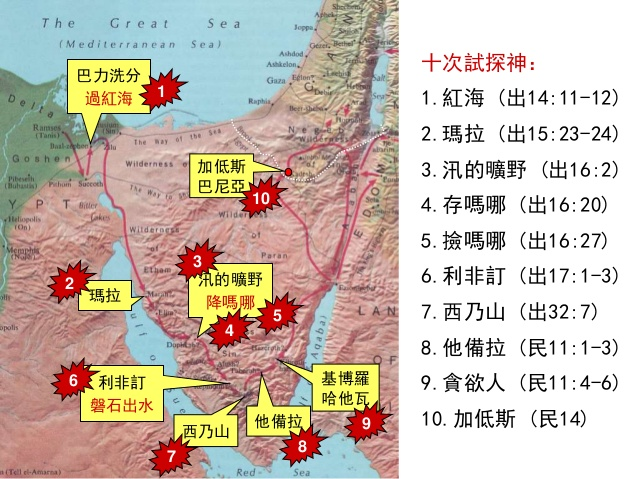
\includegraphics[width=5.in]{AMoXiFigs/minshuji/fig3}
\caption{圖1：各支派族長，人數及位置}
\label{fig:1} 
\end{center}
\end{figure}
以色列人離開耶和華的山，往前行了三天的路程。耶和華的約櫃在前頭行了三天的路程，為他們尋找安歇的地方。他們拔營往前行，日間有耶和華的雲彩在他們以上。

\subsubsection{摩西在約櫃前行停住時候的祷告 10:35-36}
約櫃往前行的時候，摩西就說：「耶和華啊，求你興起！願你的仇敵四散，願恨你的人從你面前逃跑！」約櫃停住的時候，他就說：「耶和華啊，求你回到以色列的千萬人中！」


\section{从西乃至摩押平原 11-20}

\subsection{眾百姓的叛乱-他備拉發怨言 11:1-3}
%\subsubsection{他備拉眾百姓發怨言 11:1-3}
眾百姓發怨言，他們的惡語達到耶和華的耳中。耶和華聽見了就怒氣發作，使火在他們中間焚燒，直燒到營的邊界。百姓向摩西哀求，摩西祈求耶和華，火就熄了。那地方便叫做他備拉，因為耶和華的火燒在他們中間。


\subsection{眾百姓的叛乱-基博羅哈他瓦抱怨嗎哪的貪慾之人 11:4-34}
\subsubsection{以色列人因嗎哪单调發怨言 11:4-6}
他們中間的閒雜人大起貪慾的心。以色列人又哭號說：「誰給我們肉吃呢？我們記得在埃及的時候不花錢就吃魚，也記得有黃瓜、西瓜、韭菜、蔥、蒜。 現在我們的心血枯竭了，除這嗎哪以外，在我們眼前並沒有別的東西！」

\subsubsection{关于嗎哪 11:7-9}
這嗎哪彷彿芫荽子，又好像珍珠。百姓周圍行走，把嗎哪收起來，或用磨推，或用臼搗，煮在鍋中，又做成餅，滋味好像新油。夜間露水降在營中，嗎哪也隨著降下。

\subsubsection{摩西因管理百姓責任太重先神求死 11:10-15}
摩西聽見百姓各在各家的帳篷門口哭號。耶和華的怒氣便大發作，摩西就不喜悅。摩西對耶和華說：「你為何苦待僕人，我為何不在你眼前蒙恩，竟把這管理百姓的重任加在我身上呢？這百姓豈是我懷的胎，豈是我生下來的呢？你竟對我說把他們抱在懷裡，如養育之父抱吃奶的孩子，直抱到你起誓應許給他們祖宗的地去。我從哪裡得肉給這百姓吃呢？他們都向我哭號說：『你給我們肉吃吧！』管理這百姓的責任太重了，我獨自擔當不起。你這樣待我，我若在你眼前蒙恩，求你立時將我殺了，不叫我見自己的苦情。」

\subsubsection{招聚長老中七十人輔助摩西 11:16-17}
耶和華對摩西說：「你從以色列的長老中招聚七十個人，就是你所知道做百姓的長老和官長的，到我這裡來，領他們到會幕前，使他們和你一同站立。我要在那裡降臨，與你說話，也要把降於你身上的靈分賜他們，他們就和你同當這管百姓的重任，免得你獨自擔當。

\subsubsection{耶和華要百姓自潔預備明天吃肉 11:18-23}
又要對百姓說：你們應當自潔，預備明天吃肉，因為你們哭號說：『誰給我們肉吃？我們在埃及很好。』這聲音達到了耶和華的耳中，所以他必給你們肉吃。你們不止吃一天兩天，五天十天，二十天，要吃一個整月，甚至肉從你們鼻孔裡噴出來，使你們厭惡了，因為你們厭棄住在你們中間的耶和華，在他面前哭號說：『我們為何出了埃及呢？』」摩西對耶和華說：「這與我同住的百姓，步行的男人有六十萬，你還說『我要把肉給他們，使他們可以吃一個整月』？難道給他們宰了羊群牛群，或是把海中所有的魚都聚了來，就夠他們吃嗎？」耶和華對摩西說：「耶和華的膀臂豈是縮短了嗎？現在要看我的話向你應驗不應驗。」

\subsubsection{靈降在長老中七十人身上 11:24-25}
摩西出去，將耶和華的話告訴百姓，又招聚百姓的長老中七十個人來，使他們站在會幕的四圍。耶和華在雲中降臨，對摩西說話，把降於他身上的靈分賜那七十個長老。靈停在他們身上的時候，他們就受感說話，以後卻沒有再說。

\subsubsection{約書亞為靈降在營裡兩人身上而生嫉妒 11:26-30}
但有兩個人仍在營裡，一個名叫伊利達，一個名叫米達。他們本是在那些被錄的人中，卻沒有到會幕那裡去。靈停在他們身上，他們就在營裡說預言。有個少年人跑來告訴摩西說：「伊利達、米達在營裡說預言。」摩西的幫手，嫩的兒子約書亞，就是摩西所揀選的一個人，說：「請我主摩西禁止他們！」摩西對他說：「你為我的緣故嫉妒人嗎？唯願耶和華的百姓都受感說話，願耶和華把他的靈降在他們身上！」於是摩西和以色列的長老都回到營裡去。

\subsubsection{民貪食鵪鶉而遘重災 11:31-34}
有風從耶和華那裡颳起，把鵪鶉由海面颳來，飛散在營邊和營的四圍。這邊約有一天的路程，那邊約有一天的路程，離地面約有二肘。百姓起來，終日終夜，並次日一整天，捕取鵪鶉，至少的也取了十賀梅珥，為自己擺列在營的四圍。肉在他們牙齒之間尚未嚼爛，耶和華的怒氣就向他們發作，用最重的災殃擊殺了他們。那地方便叫做基博羅哈他瓦 （慾之人的墳墓），因為他們在那裡葬埋那起貪慾之心的人。 

\subsection{在哈洗錄毀謗摩西 11:35-12:15}
\subsubsection{米利暗和亞倫因古實女子毀謗摩西 11:35-12:3}
百姓從基博羅哈他瓦走到哈洗錄，就住在哈洗錄。摩西娶了古實女子為妻。米利暗和亞倫因他所娶的古實女子就毀謗他，說：「難道耶和華單與摩西說話，不也與我們說話嗎？」這話耶和華聽見了。摩西為人極其謙和，勝過世上的眾人。

\subsubsection{耶和華责备亞倫和米利暗 12:4-9}
耶和華忽然對摩西、亞倫、米利暗說：「你們三個人都出來，到會幕這裡。」他們三個人就出來了。耶和華在雲柱中降臨，站在會幕門口，召亞倫和米利暗，二人就出來了。耶和華說：「你們且聽我的話，你們中間若有先知，我耶和華必在異象中向他顯現，在夢中與他說話。我的僕人摩西不是這樣，他是在我全家盡忠的，我要與他面對面說話，乃是明說，不用謎語，並且他必見我的形象。你們毀謗我的僕人摩西，為何不懼怕呢？」耶和華就向他們二人發怒而去。

\subsubsection{米利暗長大痲瘋摩西哀求耶和華 12:10-12:15}
雲彩從會幕上挪開了，不料，米利暗長了大痲瘋，有雪那樣白。亞倫一看米利暗長了大痲瘋，就對摩西說：「我主啊！求你不要因我們愚昧犯罪，便將這罪加在我們身上。求你不要使她像那出母腹肉已半爛的死胎。」於是摩西哀求耶和華說：「神啊，求你醫治她！」耶和華對摩西說：「她父親若吐唾沫在她臉上，她豈不蒙羞七天嗎？現在要把她在營外關鎖七天，然後才可以領她進來。」於是米利暗關鎖在營外七天。百姓沒有行路，直等到把米利暗領進來。

\subsection{在巴蘭的曠野，探子報惡信 12:16-14:45}
\subsubsection{打發十二探子窺探迦南地 12:16-13:16}
\begin{wraptable}{r}{8cm}
\vspace*{-10mm}
\centering
\begin{tabular}{|c|c|c|c|}
\hline
\hline
支派 & 父親名字&探子名字&  信心 \\ \hline\hline
流便 &撒刻 & 沙母亞 &沒有\\ \hline
西緬 &何利 & 沙法 & 沒有\\ \hline
\textcolor{red}{猶大} & \textcolor{red}{耶孚尼} &\textcolor{red}{迦勒}&\textcolor{red}有\\\hline
以薩迦& 約色&以迦&沒有\\\hline
\textcolor{red}{以法蓮}& \textcolor{red}嫩&\textcolor{red}{何西阿(約書亞）}&\textcolor{red}有\\\hline
便雅憫&拉孚&帕提&沒有 \\\hline
西布倫&梭底&迦疊&沒有\\\hline
瑪拿西&穌西&迦底&沒有\\\hline
但&基瑪利&亞米利&沒有\\\hline
亞設&米迦勒&西帖&沒有\\\hline
拿弗他利&縛西&拿比&沒有\\\hline
迦得&瑪基&臼利&沒有\\\hline\hline
\end{tabular}
\caption{探子 （13：4-16）}
\end{wraptable}
以後百姓從哈洗錄起行，在巴蘭的曠野安營。耶和華曉諭摩西說：「你打發人去窺探我所賜給以色列人的迦南地，他們每支派中要打發一個人，都要做首領的。」摩西就照耶和華的吩咐，從巴蘭的曠野打發他們去。他們都是以色列人的族長。他們的名字：屬魯本支派的有撒刻的兒子沙母亞；屬西緬支派的有何利的兒子沙法；屬猶大支派的有耶孚尼的兒子迦勒；屬以薩迦支派的有約瑟的兒子以迦；屬以法蓮支派的有嫩的兒子何西阿；屬便雅憫支派的有拉孚的兒子帕提；屬西布倫支派的有梭底的兒子迦疊；約瑟的子孫，屬瑪拿西支派的有穌西的兒子迦底；屬但支派的有基瑪利的兒子亞米利；屬亞設支派的有米迦勒的兒子西帖；屬拿弗他利支派的有縛西的兒子拿比；屬迦得支派的有瑪基的兒子臼利。這就是摩西所打發窺探那地之人的名字。摩西就稱嫩的兒子何西阿為約書亞。

\subsubsection{摩西向十二探子布置任务 13:17-20}
摩西打發他們去窺探迦南地，說：「你們從南地上山地去，看那地如何，其中所住的民是強是弱，是多是少，所住之地是好是歹，所住之處是營盤是堅城。又看那地土是肥美是瘠薄，其中有樹木沒有。你們要放開膽量，把那地的果子帶些來。」那時正是葡萄初熟的時候。

\newpage
\subsubsection{十二探子巡视的路径 13:21-24}
\begin{wrapfigure}{r}{0.6\textwidth}
\vspace*{-10mm}
\begin{center} 
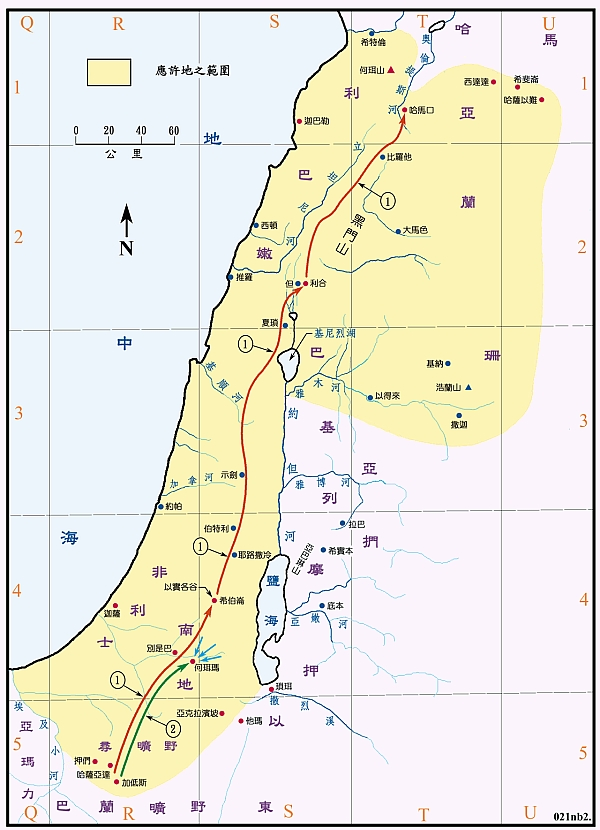
\includegraphics[width=3.8in]{AMoXiFigs/minshuji/tanzi}
\caption{1,十二探子巡视的路径;\\ 2,擅自攻打迦南人，但被迦南人擊敗}
\label{fig:1} 
\end{center}
\end{wrapfigure}
他們上去窺探那地，從尋的曠野到利合，直到哈馬口。他們從南地上去，到了希伯崙，在那裡有亞衲族人亞希幔、示篩、撻買。（原來希伯崙城被建造比埃及的鎖安城早七年。）他們到了以實各谷，從那裡砍了葡萄樹的一枝，上頭有一掛葡萄，兩個人用槓抬著，又帶了些石榴和無花果來。因為以色列人從那裡砍來的那掛葡萄，所以那地方叫做以實各谷。

\subsubsection{探子回來汇报 13:25-29}
過了四十天，他們窺探那地才回來。到了巴蘭曠野的加低斯，見摩西、亞倫並以色列的全會眾，回報摩西、亞倫並全會眾，又把那地的果子給他們看。又告訴摩西說：「我們到了你所打發我們去的那地，果然是流奶與蜜之地。這就是那地的果子。然而住那地的民強壯，城邑也堅固寬大，並且我們在那裡看見了亞衲族的人。亞瑪力人住在南地，赫人、耶布斯人、亞摩利人住在山地，迦南人住在海邊並約旦河旁。」

\subsubsection{迦勒安撫百姓 13:30-31}
迦勒在摩西面前安撫百姓，說：「我們立刻上去得那地吧，我們足能得勝！」但那些和他同去的人說：「我們不能上去攻擊那民，因為他們比我們強壯。」

\subsubsection{探子中有人報惡信 13:32-33}
探子中有人論到所窺探之地，向以色列人報惡信，說：「我們所窺探經過之地是吞吃居民之地，我們在那裡所看見的人民都身量高大。我們在那裡看見亞衲族人，就是偉人，他們是偉人的後裔。據我們看，自己就如蚱蜢一樣；據他們看，我們也是如此。」

\subsubsection{會眾大聲喧嚷百姓都哭號 14:1-4}
當下全會眾大聲喧嚷，那夜百姓都哭號。以色列眾人向摩西、亞倫發怨言，全會眾對他們說：「\textcolor{blue}{巴不得我們早死在埃及地，或是死在這曠野！耶和華為什麼把我們領到那地，使我們倒在刀下呢？我們的妻子和孩子必被擄掠。我們回埃及去豈不好嗎}？」眾人彼此說：「\textcolor{blue}{我們不如立一個首領回埃及去吧}！」

\subsubsection{約書亞和迦勒的信心 14:5-9}
\textcolor{blue}{摩西、亞倫}就俯伏在以色列全會眾面前。窺探地的人中，\textcolor{blue}{嫩的兒子約書亞}和\textcolor{blue}{耶孚尼的兒子迦勒}撕裂衣服，對以色列全會眾說：「我們所窺探經過之地是極美之地。耶和華若喜悅我們，就必將我們領進那地，把地賜給我們，那地原是流奶與蜜之地。但你們不可背叛耶和華，也不要怕那地的居民，因為他們是我們的食物，並且蔭庇他們的已經離開他們。有耶和華與我們同在，不要怕他們。」

\subsubsection{耶和華怒民違逆欲殲滅之 14:10-12}
但\textcolor{blue}{全會眾}說拿石頭打死他們二人。忽然，\textcolor{blue}{耶和華的榮光}在會幕中向以色列眾人顯現。\textcolor{blue}{耶和華對摩西說}：「這百姓藐視我要到幾時呢？我在他們中間行了這一切神蹟，他們還不信我要到幾時呢？我要用瘟疫擊殺他們，使他們不得承受那地，叫你的後裔成為大國，比他們強盛。」

\subsubsection{摩西為民求赦 14:13-19}
摩西對耶和華說：「\textcolor{blue}{埃及人必聽見}這事，因為你曾施展大能，將這百姓從他們中間領上來。埃及人要將這事傳給迦南地的居民。\textcolor{blue}{那民已經聽見}你耶和華是在這百姓中間，因為你面對面被人看見，有你的雲彩停在他們以上，你日間在雲柱中，夜間在火柱中，在他們前面行。如今你若把這百姓殺了，如殺一人，那些聽見你名聲的列邦必議論說：『耶和華因為不能把這百姓領進他向他們起誓應許之地，所以在曠野把他們殺了。』現在\textcolor{red}{求主}大顯能力，照你所說過的話說： 『耶和華不輕易發怒，並有豐盛的慈愛，赦免罪孽和過犯，萬不以有罪的為無罪，必追討他的罪，自父及子，直到三四代。』\textcolor{red}{求你}照你的大慈愛赦免這百姓的罪孽，好像你從埃及到如今常赦免他們一樣。」

\subsubsection{耶和華赦免百姓應許迦勒必得地為業 14:20-25}
耶和華說：「我照著你的話\textcolor{blue}{赦免了他們}。 然我指著我的永生起誓：遍地要被我的榮耀充滿！ 這些人雖看見我的榮耀和我在埃及與曠野所行的神蹟，仍然試探我這十次，不聽從我的話，\textcolor{blue}{他們斷不得看見}我向他們的祖宗所起誓應許之地。凡藐視我的，一個也不得看見。\\
\textcolor{red}{唯獨我的僕人迦勒}，因他另有一個心志，專一跟從我，我就把他領進他所去過的那地。\textcolor{red}{他的後裔}也必得那地為業。亞瑪力人和迦南人住在谷中，明天你們要轉回，從紅海的路往曠野去。」

\subsubsection{以色列眾發怨言者必死於野 14:26-35}
耶和華對摩西、亞倫說：「這惡會眾向我發怨言，我忍耐他們要到幾時呢？以色列人向我所發的怨言，我都聽見了。你們告訴他們：『耶和華說：我指著我的永生起誓：我必要照你們達到我耳中的話待你們。你們的屍首必倒在這曠野，並且你們中間凡被數點，從二十歲以外，向我發怨言的，必不得進我起誓應許叫你們住的那地。唯有耶孚尼的兒子迦勒和嫩的兒子約書亞才能進去。但你們的婦人孩子，就是你們所說要被擄掠的，我必把他們領進去，他們就得知你們所厭棄的那地。至於你們，你們的屍首必倒在這曠野。你們的兒女必在曠野漂流四十年，擔當你們淫行的罪，直到你們的屍首在曠野消滅。 按你們窺探那地的四十日，一年頂一日，你們要擔當罪孽四十年，就知道我與你們疏遠了。』我耶和華說過，我總要這樣待這一切聚集敵我的惡會眾。他們必在這曠野消滅，在這裡死亡。」

\subsubsection{十个報惡信探子遭瘟疫而死 14:36-38}
摩西所打發窺探那地的人回來，報那地的惡信，叫全會眾向摩西發怨言，這些報惡信的人都遭瘟疫，死在耶和華面前。其中唯有嫩的兒子約書亞和耶孚尼的兒子迦勒仍然存活。

\subsubsection{逆命的百姓欲上應許之地被殺退 14:39-45}
摩西將這些話告訴以色列眾人，他們就甚悲哀。清早起來，上山頂去，說：「我們在這裡，我們有罪了。情願上上耶和華所應許的地方去！」摩西說：「你們為何違背耶和華的命令呢？這事不能順利了！不要上去，因為耶和華不在你們中間，恐怕你們被仇敵殺敗了。亞瑪力人和迦南人都在你們面前，你們必倒在刀下。因你們退回不跟從耶和華，所以他必不與你們同在。」他們卻擅敢上山頂去，然而耶和華的約櫃和摩西沒有出營。於是亞瑪力人和住在那山上的迦南人都下來擊打他們，把他們殺退了，直到何珥瑪。

%\section{頒布律法 15 }
\subsection{頒布有關獻祭的條例 15}
\subsubsection{曉諭以色列人獻燔祭,平安祭 15:1-3}
耶和華對摩西說：「你曉諭以色列人說：你們到了我所賜給你們居住的地，若願意從牛群羊群中取牛羊做火祭獻給耶和華，無論是燔祭是平安祭，為要還特許的願，或是做甘心祭，或是逢你們節期獻的，都要奉給耶和華為馨香之祭。

\subsubsection{馨香火祭的條例 15:4-12}
\begin{wraptable}{r}{7cm}
\vspace*{-3mm}
\centering
\begin{tabular}{|c|c|c|c|}
\hline
\hline
\multirow{2}{3em}{祭物} &\multicolumn{2}{c|}{所配的素祭}&\multirow{2}{3em}{奠祭的酒(欣)} \\\cline{2-3}
  & 細麵(伊法)        &油(欣)              &\\ \hline
綿羊羔   &$\sfrac{1}{10}$ &$1\sfrac{1}{4}$&$1\sfrac{1}{4}$\\\hline
公綿羊   &$\sfrac{2}{10}$  &$1\sfrac{1}{3}$ &$1\sfrac{1}{3}$\\\hline
公牛      &$\sfrac{3}{10}$ &$\sfrac{1}{2}$    &$\sfrac{1}{2}$\\\hline
\end{tabular}
\caption{燔祭,平安祭,還特許的願\\所配的素祭和奠祭的酒}
\end{wraptable}
那獻供物的就要將細麵伊法十分之一，並油一欣四分之一，調和做素祭，獻給耶和華。無論是燔祭是平安祭，你要為每隻綿羊羔一同預備奠祭的酒一欣四分之一；為公綿羊預備細麵伊法十分之二，並油一欣三分之一，調和做素祭，又用酒一欣三分之一做奠祭，獻給耶和華為馨香之祭。你預備公牛做燔祭或是做平安祭，為要還特許的願，或是做平安祭，獻給耶和華，就要把細麵伊法十分之三，並油半欣，調和做素祭，和公牛一同獻上，又用酒半欣做奠祭，獻給耶和華為馨香的火祭。獻公牛、公綿羊、綿羊羔、山羊羔，每隻都要這樣辦理。照你們所預備的數目，按著隻數都要這樣辦理。

\subsubsection{同居的外人都歸一例 15:13-16}
凡本地人將馨香的火祭獻給耶和華，都要這樣辦理。若有外人和你們同居，或有人世世代代住在你們中間，願意將馨香的火祭獻給耶和華，你們怎樣辦理，他也要照樣辦理。至於會眾，你們和同居的外人都歸一例，作為你們世世代代永遠的定例。在耶和華面前，你們怎樣，寄居的也要怎樣。你們並與你們同居的外人當有一樣的條例，一樣的典章。

\subsubsection{舉祭的條例 15:17-21}
耶和華對摩西說：你曉諭以色列人說：你們到了我所領你們進去的那地，吃那地的糧食，就要把舉祭獻給耶和華。你們要用初熟的麥子磨麵，做餅當舉祭奉獻，你們舉上，好像舉禾場的舉祭一樣。你們世世代代要用初熟的麥子磨麵，當舉祭獻給耶和華。

\subsubsection{以色列全會眾誤犯罪獻祭的條例 15:22-26}
你們有錯誤的時候，不守耶和華所曉諭摩西的這一切命令，就是耶和華藉摩西一切所吩咐你們的，自那日以至你們的世世代代，若有誤行，是會眾所不知道的，後來全會眾就要
\vspace*{-2mm}
\begin{itemize} 
\itemsep-.35em
\item 將一隻公牛犢做燔祭，並照典章把素祭和奠祭一同獻給耶和華為馨香之祭，
\item 又獻一隻公山羊做贖罪祭。祭司要為以色列全會眾贖罪，
\end{itemize}
\vspace*{-2mm}
他們就必蒙赦免，因為這是錯誤。他們又因自己的錯誤，把供物，就是向耶和華獻的火祭和贖罪祭，一併奉到耶和華面前。以色列全會眾和寄居在他們中間的外人就必蒙赦免，因為這罪是百姓誤犯的。

\subsubsection{一個人誤犯罪獻祭的條例 15:27-29}
若有一個人誤犯了罪，他就要獻一歲的母山羊做贖罪祭。那誤行的人犯罪的時候，祭司要在耶和華面前為他贖罪，他就必蒙赦免。以色列中的本地人和寄居在他們中間的外人，若誤行了什麼事，必歸一樣的條例。

%\subsection{獻祭也不得赦免的罪 15:30-31 }
\subsubsection{違背耶和華的命令的總要剪除 15:30-31}
但那擅敢行事的，無論是本地人是寄居的，他褻瀆了耶和華，必從民中剪除。因他藐視耶和華的言語，違背耶和華的命令，那人總要剪除。他的罪孽要歸到他身上。

\subsubsection{違反安息日的條例 15:32-36 }
以色列人在曠野的時候，遇見一個人在安息日撿柴。遇見他撿柴的人，就把他帶到摩西、亞倫並全會眾那裡，將他收在監內，因為當怎樣辦他，還沒有指明。耶和華吩咐摩西說：「總要把那人治死，全會眾要在營外用石頭把他打死。」於是全會眾將他帶到營外，用石頭打死他，是照耶和華所吩咐摩西的。

\subsubsection{衣服繸子的條例 15:37-41 }
耶和華曉諭摩西說：「你吩咐以色列人，叫他們世世代代在衣服邊上做穗子，又在底邊的穗子上釘一根藍細帶子。你們佩戴這穗子，好叫你們看見就記念遵行耶和華一切的命令，不隨從自己的心意眼目行邪淫，像你們素常一樣，使你們記念遵行我一切的命令，成為聖潔，歸於你們的神。我是耶和華你們的神，曾把你們從埃及地領出來，要做你們的神。我是耶和華你們的神。」

%\section{安營時發生的事 16-17 }
\subsection{可拉黨叛亂 16-17}
\subsubsection{可拉並以色列會中250首領叛逆 16:1-3}
\begin{wraptable}{r}{9cm}
\vspace*{-20mm}
\centering
\begin{tabular}{|c|c|c|c|}
\hline
\hline
支派 & 父親名字&背叛人的名字&  結局 \\ \hline\hline
利未 &哥轄的兒子以斯哈 & 可拉 &被地開口吞沒\\ \hline
流便 & 以利押    &大坍&被地開口吞沒\\\hline
流便 & 以利押    &亞比蘭&被地開口吞沒\\\hline
流便 & 比勒    &安&被地開口吞沒\\\hline
以色列& -& 250個眾首領 &被火燒滅\\\hline
以色列& -& 14700百姓 &被瘟疫所殺\\\hline\hline
\end{tabular}
\caption{背叛的人}
\end{wraptable}
利未的曾孫、哥轄的孫子、以斯哈的兒子可拉，和魯本子孫中以利押的兒子大坍、亞比蘭，與比勒的兒子安，並以色列會中的二百五十個首領，就是有名望選入會中的人，在摩西面前一同起來，聚集攻擊摩西、亞倫，說：「你們擅自專權。全會眾個個既是聖潔，耶和華也在他們中間，你們為什麼自高，超過耶和華的會眾呢？」

\subsubsection{摩西两次劝慰可拉和他一黨的人 16:4-11}
摩西聽見這話就俯伏在地，對可拉和他一黨的人說：「到了早晨，耶和華必指示誰是屬他的，誰是聖潔的，就叫誰親近他。他所揀選的是誰，必叫誰親近他。可拉啊，你們要這樣行：你和你的一黨要拿香爐來，明日在耶和華面前，把火盛在爐中，把香放在其上。耶和華揀選誰，誰就為聖潔。你們這利未的子孫擅自專權了！」 
摩西又對可拉說：「利未的子孫哪，你們聽我說。以色列的神從以色列會中將你們分別出來，使你們親近他，辦耶和華帳幕的事，並站在會眾面前替他們當差。耶和華又使你，和你一切弟兄利未的子孫，一同親近他，這豈為小事，你們還要求祭司的職任嗎？你和你一黨的人聚集是要攻擊耶和華，亞倫算什麼，你們竟向他發怨言呢？」

\subsubsection{流便首領大坍、亞比蘭抗摩西命 16:12-14}
摩西打發人去召以利押的兒子大坍、亞比蘭。他們說：「我們不上去。你將我們從流奶與蜜之地領上來，要在曠野殺我們，這豈為小事，你還要自立為王轄管我們嗎？並且你沒有將我們領到流奶與蜜之地，也沒有把田地和葡萄園給我們為業。難道你要剜這些人的眼睛嗎？我們不上去。」

\subsubsection{亞倫和可拉黨250人各拿香爐全會眾在會幕門前 16:15-19}
摩西就甚發怒，對耶和華說：「求你不要享受他們的供物。我並沒有奪過他們一匹驢，也沒有害過他們一個人。」摩西對可拉說：「明天你和你一黨的人，並亞倫，都要站在耶和華面前。各人要拿一個香爐，共二百五十個，把香放在上面，到耶和華面前。你和亞倫也各拿自己的香爐。」於是他們各人拿一個香爐，盛上火，加上香，同摩西、亞倫站在會幕門前。可拉招聚全會眾到會幕門前，要攻擊摩西、亞倫。

\subsubsection{摩西、亞倫为全會眾代求 16:20-22}
耶和華的榮光就向全會眾顯現。耶和華曉諭摩西、亞倫說：「你們離開這會眾，我好在轉眼之間把他們滅絕。」摩西、亞倫就俯伏在地，說：「神，萬人之靈的神啊！一人犯罪，你就要向全會眾發怒嗎？」 

\subsubsection{摩西照神吩咐警戒會眾離開可拉、大坍、亞比蘭帳篷 16:23-27}
耶和華曉諭摩西說：「你吩咐會眾說：你們離開可拉、大坍、亞比蘭帳篷的四圍。」摩西起來，往大坍、亞比蘭那裡去，以色列的長老也隨著他去。他吩咐會眾說：「你們離開這惡人的帳篷吧，他們的物件，什麼都不可摸，恐怕你們陷在他們的罪中，與他們一同消滅。」於是眾人離開可拉、大坍、亞比蘭帳篷的四圍。大坍、亞比蘭帶著妻子、兒女、小孩子，都出來，站在自己的帳篷門口。

\subsubsection{摩西宣布他們活活地墜落陰間 16:28-30}
摩西說：「我行的這一切事本不是憑我自己心意行的，乃是耶和華打發我行的，必有證據使你們知道。這些人死若與世人無異，或是他們所遭的與世人相同，就不是耶和華打發我來的。倘若耶和華創作一件新事，使地開口，把他們和一切屬他們的都吞下去，叫他們活活地墜落陰間，你們就明白這些人是藐視耶和華了。」

\subsubsection{地開口把他們並一切屬可拉的人丁、財物，都吞下去 16:31-34}
摩西剛說完了這一切話，他們腳下的地就開了口，把他們和他們的家眷，並一切屬可拉的人丁、財物，都吞下去。這樣，他們和一切屬他們的都活活地墜落陰間。地口在他們上頭照舊合閉，他們就從會中滅亡。在他們四圍的以色列眾人聽他們呼號，就都逃跑，說：「恐怕地也把我們吞下去！」

\subsubsection{火燒獻香的250人，以利亞撒用香爐的銅包壇 16:35-40}
又有火從耶和華那裡出來，燒滅了那獻香的二百五十個人。耶和華曉諭摩西說：「你吩咐祭司亞倫的兒子以利亞撒從火中撿起那些香爐來，把火撒在別處，因為那些香爐是聖的。把那些犯罪自害己命之人的香爐，叫人錘成片子，用以包壇。那些香爐本是他們在耶和華面前獻過的，所以是聖的，並且可以給以色列人做記號。」於是祭司以利亞撒將被燒之人所獻的銅香爐拿來，人就錘出來，用以包壇，給以色列人做紀念，使亞倫後裔之外的人不得近前來在耶和華面前燒香，免得他遭可拉和他一黨所遭的。這乃是照耶和華藉著摩西所吩咐的。

\subsubsection{以色列全會眾發怨言，摩西、亞倫代求 16:41-45}
第二天，以色列全會眾都向摩西、亞倫發怨言說：「你們殺了耶和華的百姓了！」會眾聚集攻擊摩西、亞倫的時候，向會幕觀看，不料，有雲彩遮蓋了，耶和華的榮光顯現。摩西、亞倫就來到會幕前。耶和華吩咐摩西說：「你們離開這會眾，我好在轉眼之間把他們滅絕。」他們二人就俯伏於地。 

\subsubsection{因發怨言民遭疫癘 16:46-50}
摩西對亞倫說：「拿你的香爐，把壇上的火盛在其中，又加上香，快快帶到會眾那裡，為他們贖罪。因為有憤怒從耶和華那裡出來，瘟疫已經發作了。」亞倫照著摩西所說的拿來，跑到會中，不料，瘟疫在百姓中已經發作了。他就加上香，為百姓贖罪。他站在活人死人中間，瘟疫就止住了。除了因可拉事情死的以外，遭瘟疫死的，共有一萬四千七百人。亞倫回到會幕門口，到摩西那裡，瘟疫已經止住了。

\subsubsection{十二首領按支派各取仗存在法櫃的帳幕內 17:1-7}
耶和華對摩西說：「你曉諭以色列人，從他們手下取杖，每支派一根。從他們所有的首領，按著支派，共取十二根。你要將各人的名字寫在各人的杖上，並要將亞倫的名字寫在利未的杖上，因為各族長必有一根杖。你要把這些杖存在會幕內法櫃前，就是我與你們相會之處。後來我所揀選的那人，他的杖必發芽。這樣，我必使以色列人向你們所發的怨言止息，不再達到我耳中。」於是摩西曉諭以色列人，他們的首領就把杖交給他，按著支派，每首領一根，共有十二根，亞倫的杖也在其中。摩西就把杖存在法櫃的帳幕內，在耶和華面前。

\subsubsection{亞倫之杖發芽開花結熟杏 17:8-11}
第二天，摩西進法櫃的帳幕去。誰知利未族亞倫的杖已經發了芽，生了花苞，開了花，結了熟杏。摩西就把所有的杖從耶和華面前拿出來，給以色列眾人看。他們看見了，各首領就把自己的杖拿去。耶和華吩咐摩西說：「把亞倫的杖還放在法櫃前，給這些背叛之子留做記號。這樣，你就使他們向我發的怨言止息，免得他們死亡。」摩西就這樣行。耶和華怎樣吩咐他，他就怎樣行了。

\subsubsection{以色列說“凡挨近耶和華帳幕的是必死的” 17:12-13}
以色列人對摩西說：「我們死啦！我們滅亡啦！都滅亡啦！凡挨近耶和華帳幕的是必死的。我們都要死亡嗎？」

\subsection{頒布祭司與利未人的律法 18-19 }
\subsubsection{祭司與利未人的職任 18:1-7 }
\noindent
耶和華對亞倫說：「你和你的兒子並你本族的人，要一同擔當干犯聖所的罪孽，你和你的兒子也要一同擔當干犯祭司職任的罪孽。你要帶你弟兄利未人，就是你祖宗支派的人前來，使他們與你聯合，服侍你，只是你和你的兒子，要一同在法櫃的帳幕前供職。他們要守所吩咐你的，並守全帳幕，只是不可挨近聖所的器具和壇，免得他們和你們都死亡。他們要與你聯合，也要看守會幕，辦理帳幕一切的事，只是外人不可挨近你們。你們要看守聖所和壇，免得憤怒再臨到以色列人。我已將你們的弟兄利未人，從以色列人中揀選出來歸耶和華，是給你們為賞賜的，為要辦理會幕的事。你和你的兒子要為一切屬壇和幔子內的事一同守祭司的職任。你們要這樣供職。我將祭司的職任給你們當做賞賜侍奉我。凡挨近的外人必被治死。」

\subsubsection{祭司當得之物  18:8-14 }
耶和華曉諭亞倫說：我已將歸我的舉祭，就是以色列人一切分別為聖的物，交給你經管。因你受過膏，把這些都賜給你和你的子孫，當做永得的份。
\begin{itemize} 
\itemsep-.25em  
\item 以色列人歸給我至聖的供物，就是一切的素祭、贖罪祭、贖愆祭，其中所有存留不經火的，都為至聖之物，要歸給你和你的子孫。你要拿這些當至聖物吃，\textcolor{blue}{凡男丁都可以吃}。你當以此物為聖。
\item 以色列人所獻的舉祭並搖祭都是你的，我已賜給你和你的兒女，當做永得的份。凡在你\textcolor{blue}{家中的潔淨人都可以吃}。凡油中、新酒中、五穀中至好的，就是以色列人所獻給耶和華初熟之物，我都賜給你。凡從他們地上所帶來給耶和華初熟之物，也都要歸於你。你家中的潔淨人都可以吃。以色列中一切永獻的都必歸於你。 
\end{itemize}

\subsubsection{頭生之物 18:15-20}
\begin{itemize} 
\itemsep-.25em  
\item 他們所有奉給耶和華的，連人帶牲畜，凡頭生的，都要歸給你。只是人頭生的，總要贖出來，不潔淨牲畜頭生的也要贖出來。其中在一月之外所當贖的，要照你所估定的價，按聖所的平，用銀子五舍客勒贖出來（一舍客勒是二十季拉）。 
\item 只是頭生的牛，或是頭生的綿羊和山羊，必不可贖，都是聖的，要把牠的血灑在壇上，把牠的脂油焚燒，當做馨香的火祭獻給耶和華。牠的肉必歸你，像被搖的胸、被舉的右腿歸你一樣。凡以色列人所獻給耶和華聖物中的舉祭，我都賜給你和你的兒女，當做永得的份。這是給你和你的後裔，在耶和華面前作為永遠的鹽(不廢壞)約。」
\item 耶和華對亞倫說：你在以色列人的境內不可有產業，在他們中間也不可有份。我就是你的份，是你的產業。
\end{itemize}

\subsubsection{利未人的份 18:21-24}
\begin{itemize} 
\itemsep-.25em  
\item 凡以色列中出產的十分之一，我已賜給利未的子孫為業。因他們所辦的是會幕的事，所以賜給他們為酬他們的勞。
\item 從今以後，以色列人不可挨近會幕，免得他們擔罪而死。唯獨利未人要辦會幕的事，擔當罪孽，這要做你們世世代代永遠的定例。
\item 他們在以色列人中不可有產業。因為以色列人中出產的十分之一，就是獻給耶和華為舉祭的，我已賜給利未人為業，所以我對他們說：在以色列人中不可有產業。」
\end{itemize}

\subsubsection{利未人的奉獻 18:25-32}
耶和華吩咐摩西說：「你曉諭利未人說：你們從以色列人中所取的十分之一，就是我給你們為業的，要再從那十分之一中取十分之一作為舉祭獻給耶和華。這舉祭要算為你們場上的穀，又如滿酒榨的酒。這樣，你們從以色列人中所得的十分之一也要做舉祭獻給耶和華，從這十分之一中，將所獻給耶和華的舉祭歸給祭司亞倫。奉給你們的一切禮物，要從其中將至好的，就是分別為聖的，獻給耶和華為舉祭。所以你要對利未人說：『你們從其中將至好的舉起，這就算為你們場上的糧，又如酒榨的酒。你們和你們家屬隨處可以吃，這原是你們的賞賜，是酬你們在會幕裡辦事的勞。你們從其中將至好的舉起，就不致因這物擔罪。你們不可褻瀆以色列人的聖物，免得死亡。』」

\subsubsection{用紅母牛灰調做除汙穢水 19:1-10}
\noindent
耶和華曉諭摩西、亞倫說： 「耶和華命定律法中的一條律例乃是這樣說：你要吩咐以色列人，把一隻沒有殘疾、未曾負軛、純紅的母牛牽到你這裡來，交給祭司以利亞撒。他必牽到營外，人就把牛宰在他面前。 祭司以利亞撒要用指頭蘸這牛的血，向會幕前面彈七次。人要在他眼前把這母牛焚燒，牛的皮、肉、血、糞都要焚燒。祭司要把香柏木、牛膝草、朱紅色線都丟在燒牛的火中。祭司必不潔淨到晚上，要洗衣服，用水洗身，然後可以進營。 燒牛的人必不潔淨到晚上，也要洗衣服，用水洗身。必有一個潔淨的人收起母牛的灰，存在營外潔淨的地方，為以色列會眾調做除汙穢的水，這本是除罪的。收起母牛灰的人必不潔淨到晚上，要洗衣服。這要給以色列人和寄居在他們中間的外人作為永遠的定例。 

\subsubsection{適用除汙水的人 19:11-16}
\begin{itemize} 
\itemsep-.25em  
\item 摸了人死屍的，就必七天不潔淨。那人到第三天要用這除汙穢的水潔淨自己，第七天就潔淨了。他若在第三天不潔淨自己，第七天就不潔淨了。凡摸了人死屍，不潔淨自己的，就玷汙了耶和華的帳幕，這人必從以色列中剪除。因為那除汙穢的水沒有灑在他身上，他就為不潔淨，汙穢還在他身上。
\item 人死在帳篷裡的條例乃是這樣：凡進那帳篷的和一切在帳篷裡的，都必七天不潔淨。凡敞口的器皿，就是沒有紮上蓋的，也是不潔淨。
\item 無論何人在田野裡摸了被刀殺的，或是屍首，或是人的骨頭，或是墳墓，就要七天不潔淨。
\end{itemize}

\subsubsection{除汙水的使用 19:17-22}
要為這不潔淨的人拿些燒成的除罪灰放在器皿裡倒上活水。必當有一個潔淨的人拿牛膝草蘸在這水中，把水灑在帳篷上和一切器皿並帳篷內的眾人身上，又灑在摸了骨頭，或摸了被殺的，或摸了自死的，或摸了墳墓的那人身上。
\vspace*{-2mm}
\begin{itemize} 
\itemsep-.25em  
\item 第三天和第七天，潔淨的人要灑水在不潔淨的人身上，第七天就使他成為潔淨。那人要洗衣服，用水洗澡，到晚上就潔淨了。
\item 但那汙穢而不潔淨自己的，要將他從會中剪除，因為他玷汙了耶和華的聖所。除汙穢的水沒有灑在他身上，他是不潔淨的。這要給你們作為永遠的定例。
\item 並且那灑除汙穢水的人要洗衣服，凡摸除汙穢水的，必不潔淨到晚上。不潔淨人所摸的一切物就不潔淨，摸了這物的人必不潔淨到晚上。
\end{itemize}

%\section{行程中發生的事 20-27 }
\subsection{旷野漂流中發生的事 20-22}
\subsubsection{正月米利暗死在尋的曠野加低斯 20:1}
\begin{wrapfigure}{r}{0.5\textwidth}
\vspace*{-30mm}
\center 
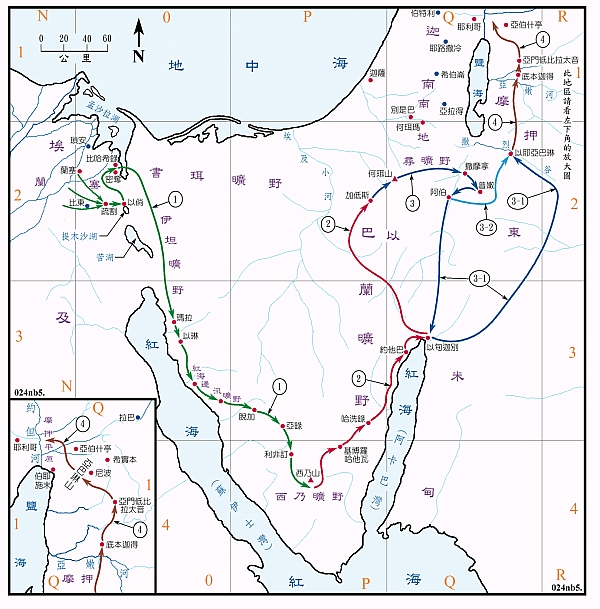
\includegraphics[width=3.5in]{AMoXiFigs/fig4}
\caption{行程中發生的事}
\label{fig:1} 
%\end{center}
\end{wrapfigure}
正月間，以色列全會眾到了尋的曠野，就住在加低斯。米利暗死在那裡，就葬在那裡。


\subsubsection{米利巴摩西因无水受牵累 20:2-13}
\subsubsubsection{米利巴會眾无水攻擊摩西 20:2-5}
會眾沒有水喝，就聚集攻擊摩西、亞倫。百姓向摩西爭鬧說：「我們的弟兄曾死在耶和華面前，我們恨不得與他們同死。你們為何把耶和華的會眾領到這曠野，使我們和牲畜都死在這裡呢？你們為何逼著我們出埃及，領我們到這壞地方呢？這地方不好撒種，也沒有無花果樹、葡萄樹、石榴樹，又沒有水喝。」

\subsubsubsection{曉諭摩西吩咐磐石出水 20:6-9}
摩西、亞倫離開會眾，到會幕門口，俯伏在地。耶和華的榮光向他們顯現。耶和華曉諭摩西說：「你拿著杖去，和你的哥哥亞倫招聚會眾，在他們眼前吩咐磐石發出水來，水就從磐石流出，給會眾和他們的牲畜喝。」

\subsubsubsection{摩西擊打磐石受亏损 20:10-13 }
\begin{table}[H]
%\arrayrulecolor[HTML]{DB5800}
\begin{threeparttable}
\begin{tabular}{@{}p{0.53\textwidth}*{4}{L{\dimexpr0.6\linewidth-10\tabcolsep\relax}}@{}}
\toprule
摩西 &  以東王 \\\hline
於是摩西照耶和華所吩咐的，從耶和華面前取了杖去。摩西、亞倫就招聚會眾到磐石前。摩西說：「你們這些背叛的人聽我說：我為你們使水從這磐石中流出來嗎？」摩西舉手，用杖擊打磐石兩下，就有許多水流出來，會眾和他們的牲畜都喝了。
&耶和華對摩西、亞倫說：「因為你們不信我，不在以色列人眼前尊我為聖，所以你們必不得領這會眾進我所賜給他們的地去。」這水名叫米利巴(爭鬧)水，是因以色列人向耶和華爭鬧，耶和華就在他們面前顯為聖。\tabularnewline
\bottomrule
\end{tabular}
\caption{摩西擊打磐石受亏损}
\end{threeparttable}
\end{table} 

\subsubsection{以東王不允以色列人過其境 20:14-21}
\begin{table}[H]
%\arrayrulecolor[HTML]{DB5800}
\begin{threeparttable}
\begin{tabular}{@{}p{0.53\textwidth}*{4}{L{\dimexpr0.58\linewidth-10\tabcolsep\relax}}@{}}
\toprule
摩西 &  以東王 \\\hline
摩西從加低斯差遣使者去見以東王，說：「你的弟兄以色列人這樣說：我們所遭遇的一切艱難，就是我們的列祖下到埃及，我們在埃及久住，埃及人惡待我們的列祖和我們，我們哀求耶和華的時候，他聽了我們的聲音，差遣使者把我們從埃及領出來，這事你都知道。如今，我們在你邊界上的城加低斯。求你容我們從你的地經過。我們不走田間和葡萄園，也不喝井裡的水，只走大道(王道)，不偏左右，直到過了你的境界。」
&以東王說：「你不可從我的地經過，免得我帶刀出去攻擊你。」\tabularnewline\hline
以色列人說：「我們要走大道上去。我們和牲畜若喝你的水，必給你價值。不求別的，只求你容我們步行過去。」
&以東王說：「你們不可經過。」就率領許多人出來，要用強硬的手攻擊以色列人。這樣，以東王不肯容以色列人從他的境界過去。於是他們轉去，離開他。\tabularnewline
\bottomrule
\end{tabular}
\caption{以東王不允以色列人過其境}
\end{threeparttable}
\end{table} 

\subsubsection{亞倫死在何珥山 20:22-29 }
以色列全會眾從加低斯起行，到了何珥山。耶和華在附近以東邊界的何珥山上曉諭摩西、亞倫說：「亞倫要歸到他列祖(本民)那裡。他必不得入我所賜給以色列人的地，因為在米利巴水，你們違背了我的命。你帶亞倫和他的兒子以利亞撒上何珥山，把亞倫的聖衣脫下來，給他的兒子以利亞撒穿上。亞倫必死在那裡，歸他列祖。」摩西就照耶和華所吩咐的行。三人當著會眾的眼前上了何珥山。摩西把亞倫的聖衣脫下來，給他的兒子以利亞撒穿上，亞倫就死在山頂那裡。於是摩西和以利亞撒下了山。全會眾，就是以色列全家，見亞倫已經死了，便都為亞倫哀哭了三十天。
 
\subsubsection{何珥瑪的迦南人亞拉得王被毀 21:1-3 }
\noindent
南地的迦南人亞拉得王、聽說以色列人從亞他林路來、就和以色列人爭戰、擄了他們幾個人。耶和華應允了以色列人、他們就把迦南人、和迦南人的城邑、盡行毀滅。那地方的名便叫何珥瑪〔毀滅〕。 

\subsubsection{製造銅火蛇  21:5-9 }
他們從何珥山起行，往紅海那條路走，要繞過以東地。百姓因這路難行，心中甚是煩躁，就怨讟神和摩西說：「你們為什麼把我們從埃及領出來，使我們死在曠野呢？這裡沒有糧，沒有水，我們的心厭惡這淡薄的食物！」於是耶和華使火蛇進入百姓中間，蛇就咬他們，以色列人中死了許多。百姓到摩西那裡，說：「我們怨讟耶和華和你，有罪了。求你禱告耶和華，叫這些蛇離開我們。」於是摩西為百姓禱告。耶和華對摩西說：「你製造一條火蛇，掛在杆子上。凡被咬的，一望這蛇，就必得活。」摩西便製造一條銅蛇，掛在杆子上。凡被蛇咬的，一望這銅蛇就活了。

\subsubsection{曠野路線 21:10-20 }
以色列人起行，安營在阿伯。又從阿伯起行，安營在以耶亞巴琳，與摩押相對的曠野，向日出之地。從那裡起行，安營在撒烈谷。從那裡起行，安營在亞嫩河那邊。這亞嫩河是在曠野，從亞摩利的境界流出來的。原來亞嫩河是摩押的邊界，在摩押和亞摩利人搭界的地方。所以《耶和華的戰記》上說：「蘇法的哇哈伯與亞嫩河的谷，並向亞珥城眾谷的下坡，是靠近摩押的境界。」以色列人從那裡起行，到了比珥(井)。從前耶和華吩咐摩西說：「招聚百姓，我好給他們水喝」，說的就是這井。當時，以色列人唱歌說：「井啊，湧上水來！你們要向這井歌唱。這井是首領和民中的尊貴人用圭用杖所挖所掘的。」以色列人從曠野往瑪他拿去，從瑪他拿到拿哈列，從拿哈列到巴末，從巴末到摩押地的谷，又到那下望曠野之毗斯迦的山頂。

\subsubsection{希實本的亞摩利人王西宏 21:21-32}
以色列人差遣使者去見亞摩利人的王西宏，說：「求你容我們從你的地經過。我們不偏入田間和葡萄園，也不喝井裡的水，只走大道 (王道)，直到過了你的境界。」西宏不容以色列人從他的境界經過，就招聚他的眾民出到曠野，要攻擊以色列人，到了雅雜與以色列人爭戰。以色列人用刀殺了他，得了他的地，從亞嫩河到雅博河，直到亞捫人的境界，因為亞捫人的境界多有堅壘。以色列人奪取這一切的城邑，也住亞摩利人的城邑，就是希實本與希實本的一切鄉村。這希實本是亞摩利王西宏的京城，西宏曾與摩押的先王爭戰，從他手中奪取了全地，直到亞嫩河。所以那些作詩歌的說：「你們來到希實本，願西宏的城被修造，被建立！因為有火從希實本發出，有火焰出於西宏的城，燒盡摩押的亞珥和亞嫩河丘壇的祭司(主)。摩押啊，你有禍了！基抹的民哪，你們滅亡了！基抹的男子逃奔，女子被擄，交付亞摩利的王西宏。我們射了他們，希實本直到底本盡皆毀滅。我們使地變成荒場，直到挪法。這挪法直延到米底巴。」這樣，以色列人就住在亞摩利人之地。摩西打發人去窺探雅謝，以色列人就占了雅謝的鎮市，趕出那裡的亞摩利人。

\subsubsection{巴珊王噩 21:33-35}
以色列人轉回，向巴珊去。巴珊王噩和他的眾民都出來，在以得來與他們交戰。耶和華對摩西說：「不要怕他。因我已將他和他的眾民，並他的地，都交在你手中。你要待他像從前待住希實本的亞摩利王西宏一般。」於是他們殺了他和他的眾子，並他的眾民，沒有留下一個，就得了他的地。

\section{摩押平原的事件 22-36}
\subsection{摩押王西撥的兒子召巴勒比珥的兒子巴蘭22-25}

\subsubsection{摩押王西撥的兒子求米甸長老召巴蘭 22:1-6}
以色列人起行，在摩押平原，約旦河東，對著耶利哥安營。以色列人向亞摩利人所行的一切事，西撥的兒子巴勒都看見了。摩押人因以色列民甚多，就大大懼怕，心內憂急，對米甸的長老說：「現在這眾人要把我們四圍所有的一概舔盡，就如牛舔盡田間的草一般。」那時西撥的兒子巴勒做摩押王。他差遣使者往大河邊的毗奪去，到比珥的兒子巴蘭本鄉那裡，召巴蘭來，說：「有一宗民從埃及出來，遮滿地面，與我對居。這民比我強盛，現在求你來為我咒詛他們，或者我能得勝，攻打他們，趕出此地。因為我知道，你為誰祝福，誰就得福；你咒詛誰，誰就受咒詛。」

\subsubsection{一次差摩押米甸長老召巴蘭被拒 22:7-14}
\begin{itemize} 
\itemsep-.35em
\item 摩押的長老和米甸的長老手裡拿著卦金，到了巴蘭那裡，將巴勒的話都告訴了他。巴蘭說：「你們今夜在這裡住宿，我必照耶和華所曉諭我的回報你們。」摩押的使臣就在巴蘭那裡住下了。
\item 神臨到巴蘭那裡，說：「在你這裡的人都是誰？」巴蘭回答說：「是摩押王西撥的兒子巴勒打發人到我這裡來，說： 『從埃及出來的民遮滿地面，你來為我咒詛他們，或者我能與他們爭戰，把他們趕出去。』」神對巴蘭說：「你不可同他們去，也不可咒詛那民，因為那民是蒙福的。」
\item 巴蘭早晨起來，對巴勒的使臣說：「你們回本地去吧，因為耶和華不容我和你們同去。」摩押的使臣就起來，回巴勒那裡去，說：「巴蘭不肯和我們同來。」
\end{itemize}

\subsubsection{二次差更多且尊貴的人召巴蘭 22:15-20}
\begin{itemize} 
\itemsep-.35em
\item 巴勒又差遣使臣，比先前的又多又尊貴。他們到了巴蘭那裡，對他說：「西撥的兒子巴勒這樣說：求你不容什麼事攔阻你不到我這裡來！因為我必使你得極大的尊榮，你向我要什麼，我就給你什麼，只求你來為我咒詛這民。」
\item 巴蘭回答巴勒的臣僕說：「巴勒就是將他滿屋的金銀給我，我行大事小事也不得越過耶和華我神的命。現在我請你們今夜在這裡住宿，等我得知耶和華還要對我說什麼。」
\item 當夜，神臨到巴蘭那裡，說：「這些人若來召你，你就起來同他們去，你只要遵行我對你所說的話。」
\end{itemize}

\subsubsection{天使阻巴蘭 22:21-27}
\begin{table}[H]
\begin{tabular}{@{}p{0.385\textwidth}*{4}{L{\dimexpr0.735\linewidth-10\tabcolsep\relax}}@{}}
\toprule
巴蘭 &驢 \\\hline
巴蘭早晨起來，備上驢，和摩押的使臣一同去了。神因他去就發了怒，耶和華的使者站在路上抵擋他。他騎著驢有兩個僕人跟隨他。&驢看見耶和華的使者站在路上，手裡有拔出來的刀，就從路上跨進田間。\\\hline
巴蘭便打驢，要叫牠回轉上路。&耶和華的使者就站在葡萄園的窄路上，這邊有牆，那邊也有牆。 驢看見耶和華的使者，就貼靠牆，將巴蘭的腳擠傷了。\\\hline
巴蘭又打驢。&耶和華的使者又往前去，站在狹窄之處，左右都沒有轉折的地方。驢看見耶和華的使者，就臥在巴蘭底下，\tabularnewline\hline
巴蘭發怒，用杖打驢。&耶和華叫驢開口對巴蘭說：「我向你行了什麼，你竟打我這三次呢？」\tabularnewline\hline
巴蘭對驢說：「因為你戲弄我。我恨不能手中有刀，把你殺了。」&驢對巴蘭說：「我不是你從小時直到今日所騎的驢嗎？我素常向你這樣行過嗎？」\tabularnewline\hline
巴蘭說：「沒有。」&\tabularnewline\hline
\bottomrule
\end{tabular}
\caption{天使阻巴蘭,驢开口說話}
\end{table} 

\subsubsection{耶和華的使者對巴蘭說話 22:31-35}
\begin{table}[H]
%\begin{threeparttable}
\begin{tabular}{@{}p{0.63\textwidth}*{4}{L{\dimexpr0.48\linewidth-10\tabcolsep\relax}}@{}}
\toprule
耶和華的使者 &  巴蘭 \\\hline
當時，耶和華使巴蘭的眼目明亮，&他就看見耶和華的使者站在路上，手裡有拔出來的刀。巴蘭便低頭俯伏在地。\\\hline
耶和華的使者對他說：「你為何這三次打你的驢呢？我出來抵擋你，因你所行的，在我面前偏僻。驢看見我就三次從我面前偏過去，驢若沒有偏過去，我早把你殺了，留牠存活。」&巴蘭對耶和華的使者說：「我有罪了，我不知道你站在路上阻擋我。你若不喜歡我去，我就轉回。」\\\hline
耶和華的使者對巴蘭說：「你同這些人去吧，你只要說我對你說的話。」&於是巴蘭同著巴勒的使臣去了。\tabularnewline
\bottomrule
\end{tabular}
\caption{耶和華的使者對巴蘭說話}
%\end{threeparttable}
\end{table} 


\subsubsection{巴勒迎巴蘭 22:36-40}
\begin{figure}[H]%{.5\linewidth}
\centering
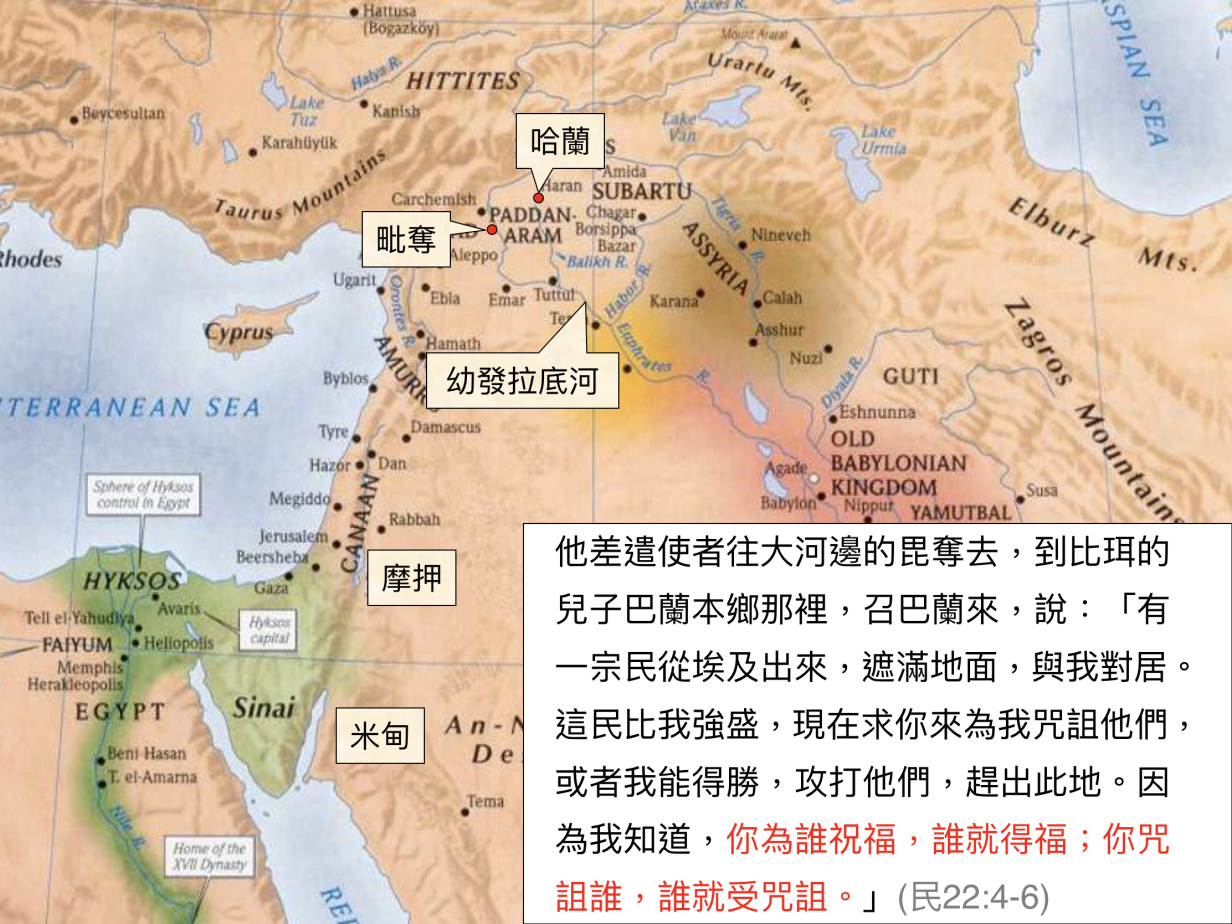
\includegraphics[width=5in]{AMoXiFigs/minshuji/balan}
\caption{以色列在曠野的經歷}
\label{fig:sub1}
\end{figure}
\begin{table}[H]
%\begin{threeparttable}
\begin{tabular}{@{}p{0.5\textwidth}*{4}{L{\dimexpr0.58\linewidth-10\tabcolsep\relax}}@{}}
\toprule
巴勒&巴蘭 \\\hline
巴勒聽見巴蘭來了，就往摩押京城去迎接他。這城是在邊界上，在亞嫩河旁。巴勒對巴蘭說：「我不是急急地打發人到你那裡去召你嗎？你為何不到我這裡來呢？我豈不能使你得尊榮嗎？」&巴蘭說：「我已經到你這裡來了。現在我豈能擅自說什麼呢？神將什麼話傳給我，我就說什麼。」巴蘭和巴勒同行，來到基列胡瑣。巴勒宰（獻）了牛羊，送給巴蘭和陪伴的使臣。\\\hline
\bottomrule
\end{tabular}
\caption{巴勒迎巴蘭}
%\end{threeparttable}
\end{table} 


\subsubsection{巴蘭第一次預言 22:41-23:12}
\begin{table}[H]
\begin{tabular}{@{}p{0.3\textwidth}*{4}{L{\dimexpr0.8\linewidth-10\tabcolsep\relax}}@{}}
\toprule
巴勒&巴蘭 \\\hline
到了早晨，巴勒領巴蘭到巴力的高處，&巴蘭從那裡觀看以色列營的邊界。巴蘭對巴勒說：「你在這裡給我築七座壇，為我預備七隻公牛、七隻公羊。」\\\hline
巴勒照巴蘭的話行了。巴勒和巴蘭在每座壇上獻一隻公牛、一隻公羊。&巴蘭對巴勒說：「你站在你的燔祭旁邊，我且往前去，或者耶和華來迎見我。他指示我什麼，我必告訴你。」於是巴蘭上一淨光的高處。\\\hline
&神迎見巴蘭。巴蘭說：「我預備了七座壇，在每座壇上獻了一隻公牛、一隻公羊。」耶和華將話傳給巴蘭，又說:「你回到巴勒那裡，要如此如此說。」 \\\hline
&他就回到巴勒那裡，見他同摩押的使臣都站在燔祭旁邊。巴蘭便題起詩歌說："巴勒引我出亞蘭，摩押王引我出東山說:『來啊，為我咒詛雅各！來啊，怒罵以色列！』神沒有咒詛的我焉能咒詛？耶和華沒有怒罵的我焉能怒罵？我從高峰看他，從小山望他，這是獨居的民，不列在萬民中。誰能數點雅各的塵土?誰能計算以色列的四分之一?我願如義人之死而死，我願如義人之終而終。"\\\hline
巴勒對巴蘭說：「你向我做的是什麼事呢？我領你來咒詛我的仇敵，不料，你竟為他們祝福！」&他回答說：「耶和華傳給我的話，我能不謹慎傳說嗎？」\\\hline
\bottomrule
\end{tabular}
\caption{巴蘭第一次預言}
\end{table} 



\subsubsection{巴蘭第二次預言 23:13-26}
\begin{table}[H]
%\begin{threeparttable}
\begin{tabular}{@{}p{0.5\textwidth}*{4}{L{\dimexpr0.63\linewidth-10\tabcolsep\relax}}@{}}
\toprule
巴勒&巴蘭 \\\hline
巴勒說：「求你同我往別處去，在那裡可以看見他們。你不能全看見，只能看見他們邊界上的人。在那裡要為我咒詛他們。」於是領巴蘭到了瑣腓田，上了毗斯迦山頂，築了七座壇，每座壇上獻一隻公牛、一隻公羊。&巴蘭對巴勒說：「你站在這燔祭旁邊，等我往那邊去迎見耶和華。」耶和華臨到巴蘭那裡，將話傳給他，又說：「你回到巴勒那裡，要如此如此說。」他就回到巴勒那裡，見他站在燔祭旁邊，摩押的使臣也和他在一處。\\\hline
巴勒問他說：「耶和華說了什麼話呢？」&巴蘭就題詩歌說：「巴勒，你起來聽；西撥的兒子，你聽我言。神非人，必不至說謊；也非人子，必不至後悔。他說話豈不照著行呢？他發言豈不要成就呢？我奉命祝福，神也曾賜福，此事我不能翻轉。他未見雅各中有罪孽，也未見以色列中有奸惡。耶和華他的神和他同在，有歡呼王的聲音在他們中間。神領他們出埃及，他們似乎有野牛之力。斷沒有法術可以害雅各，也沒有占卜可以害以色列。現在必有人論及雅各，就是論及以色列說：『神為他行了何等的大事！』這民起來彷彿母獅，挺身好像公獅，未曾吃野食，未曾喝被傷者之血，決不躺臥。」\\\hline
巴勒對巴蘭說：「你一點不要咒詛他們，也不要為他們祝福。」&巴蘭回答巴勒說：「我豈不是告訴你說，凡耶和華所說的，我必須遵行嗎？」\\\hline
\bottomrule
\end{tabular}
\caption{巴蘭第二次預言}
%\end{threeparttable}
\end{table} 


\subsubsection{巴蘭第三次預言 23:27-24:13}
\begin{table}[H]
%\begin{threeparttable}
\begin{tabular}{@{}p{0.5\textwidth}*{4}{L{\dimexpr0.63\linewidth-10\tabcolsep\relax}}@{}}
\toprule
巴勒&巴蘭 \\\hline
巴勒對巴蘭說：「來吧，我領你往別處去，或者神喜歡你在那裡為我咒詛他們。」巴勒就領巴蘭到那下望曠野的毗珥山頂上。&巴蘭對巴勒說：「你在這裡為我築七座壇，又在這裡為我預備七隻公牛、七隻公羊。」\\\hline
巴勒就照巴蘭的話行，在每座壇上獻一隻公牛、一隻公羊。&巴蘭見耶和華喜歡賜福於以色列，就不像前兩次去求法術，卻面向曠野。巴蘭舉目，看見以色列人照著支派居住，神的靈就臨到他身上，他便題起詩歌說：「比珥的兒子巴蘭說，眼目閉住（（睜開））的人說，得聽神的言語、得見全能者的異象、眼目睜開而仆倒的人說：雅各啊，你的帳篷何等華美！以色列啊，你的帳幕何其華麗！如接連的山谷，如河旁的園子，如耶和華所栽的沉香樹，如水邊的香柏木。水要從他的桶裡流出，種子要撒在多水之處。他的王必超過亞甲，他的國必要振興。神領他出埃及，他似乎有野牛之力。他要吞吃敵國，折斷他們的骨頭，用箭射透他們。他蹲如公獅，臥如母獅，誰敢惹他？凡給你祝福的，願他蒙福；凡咒詛你的，願他受咒詛。」\\\hline
巴勒向巴蘭生氣，就拍起手來，對巴蘭說：「我召你來為我咒詛仇敵，不料，你這三次竟為他們祝福。如今你快回本地去吧！我想使你得大尊榮，耶和華卻阻止你不得尊榮。」&巴蘭對巴勒說：「我豈不是對你所差遣到我那裡的使者說，巴勒就是將他滿屋的金銀給我，我也不得越過耶和華的命，憑自己的心意行好行歹？耶和華說什麼，我就要說什麼。\\\hline
\bottomrule
\end{tabular}
\caption{巴蘭第三次預言}
%\end{threeparttable}
\end{table} 

\subsubsection{巴蘭第四次預言 24:14-25}
\begin{itemize} 
\itemsep-.35em
\item 現在我要回本族去。你來，我告訴你這民日後要怎樣待你的民。」他就題起詩歌說：「比珥的兒子巴蘭說，眼目閉住（睜開）的人說，得聽神的言語、明白至高者的意旨、看見全能者的異象、眼目睜開而仆倒的人說：我看他卻不在現時，我望他卻不在近日。有星要出於雅各，有杖要興於以色列，必打破摩押的四角，毀壞擾亂之子。他必得以東為基業，又得仇敵之地西珥為產業，以色列必行事勇敢。有一位出於雅各的，必掌大權，他要除滅城中的餘民。」
\item 巴蘭觀看亞瑪力，就題起詩歌說：「亞瑪力原為諸國之首，但他終必沉淪。」
\item 巴蘭觀看基尼人，就題起詩歌說：「你的住處本是堅固，你的窩巢做在巖穴中。然而基尼必至衰微，直到亞述把你擄去。」
\item 巴蘭又題起詩歌說：「哀哉！神行這事，誰能得活？必有人乘船從基提界而來，苦害亞述，苦害希伯，他也必至沉淪。」於是巴蘭起來，回他本地去。巴勒也回去了。
\end{itemize} 

%\subsection{百姓在什亭行淫亂 25 }
\subsubsection{百姓與摩押女子在什亭行淫亂 25:1-5}
以色列人住在什亭，百姓與摩押女子行起淫亂。因為這女子叫百姓來，一同給她們的神獻祭，百姓就吃她們的祭物，跪拜她們的神。以色列人與巴力毗珥聯合，耶和華的怒氣就向以色列人發作。耶和華吩咐摩西說：「將百姓中所有的族長在我面前對著日頭懸掛，使我向以色列人所發的怒氣可以消了。」於是摩西吩咐以色列的審判官說：「凡屬你們的人，有與巴力毗珥聯合的，你們各人要把他們殺了。」




\subsubsection{非尼哈刺透行淫亂的二人止息瘟疫 25:6-9}
摩西和以色列全會眾正在會幕門前哭泣的時候，誰知，有以色列中的一個人，當他們眼前，帶著一個米甸女人到他弟兄那裡去。祭司亞倫的孫子、以利亞撒的兒子非尼哈看見了，就從會中起來，手裡拿著槍，跟隨那以色列人進亭子裡去，便將以色列人和那女人由腹中刺透。這樣，在以色列人中瘟疫就止息了。那時遭瘟疫死的有二萬四千人。

\subsubsection{神賜非尼哈後裔永遠當祭司的職任 25:10-13}
耶和華曉諭摩西說：「祭司亞倫的孫子、以利亞撒的兒子非尼哈，使我向以色列人所發的怒消了，因他在他們中間，以我的忌邪為心，使我不在忌邪中把他們除滅。因此，你要說：我將我平安的約賜給他，這約要給他和他的後裔，作為永遠當祭司職任的約，因他為神，有忌邪的心，為以色列人贖罪。」

\subsubsection{行淫亂的以色列人和米甸女人 25:14-15}
那與米甸女人一同被殺的以色列人，名叫心利，是撒路的兒子，是西緬一個宗族的首領。那被殺的米甸女人，名叫哥斯比，是蘇珥的女兒。這蘇珥是米甸一個宗族的首領。

\newpage
\subsubsection{耶和華曉諭摩西擊殺米甸 25:16-18}
\begin{wraptable}{r}{9cm}
\vspace*{-15mm}
\centering
\begin{tabular}{|c|c|c|c|c|}\hline\hline
位置 & 支派 & 第一次人數&第二次人數&  增減 \\ \hline\hline
\multirow{3}{*}{南營} & 流便 & 46500 & 43730  &-2270\\ \cline{2-5}
\multicolumn{1}{|c|}{}  &西緬 & 59300 & 22200 &-37100 \\\cline{2-5}
\multicolumn{1}{|c|}{}  &迦得&45650&40500&-5600\\\cline{2-5}
\hline
\multirow{3}{*}{東營} &猶大 & 57400    &76500& +19100\\\cline{2-5}
\multicolumn{1}{|c|}{} & 以薩迦& 54400&64300&+9900\\\cline{2-5}
\multicolumn{1}{|c|}{} & 西布倫&57400&60500&+3100\\\cline{2-5}
\hline
\multirow{3}{*}{西營} &瑪拿西&32200&52700&+20500\\\cline{2-5}
\multicolumn{1}{|c|}{} & 以法蓮&40500&32500&-8000\\\cline{2-5}
\multicolumn{1}{|c|}{} & 便雅憫&35400&45600&+10200 \\\cline{2-5}
\hline
\multirow{3}{*}{北營} &但&62700&64400&+2700\\\cline{2-5}
\multicolumn{1}{|c|}{} & 亞設&41500&53400&+11900\\\cline{2-5}
\multicolumn{1}{|c|}{} & 拿弗他利&53400&45400&-8000\\\cline{2-5}
\hline
\textbf{總數} & \textbf{以色列} & \textbf{603550}  & \textbf{601730} &
 \textbf{\textcolor{red}{-1820}}\\\hline
 & 利未& 22000 & 23000 & +1000\\\hline
\end{tabular}
\caption{第二次人數 26:1-26 }
\end{wraptable}
耶和華曉諭摩西說：「你要擾害米甸人，擊殺他們。因為他們用詭計擾害你們，在毗珥的事上和他們的姐妹米甸首領的女兒哥斯比的事上，用這詭計誘惑了你們。」這哥斯比，當瘟疫流行的日子，因毗珥的事被殺了。


\subsection{第二次數點以色列人 26:1-65}
\subsubsection{耶和華曉諭摩西以利亞撒二次點人 26:1-4}
瘟疫之後，耶和華曉諭摩西和祭司亞倫的兒子以利亞撒說： 「你們要將以色列全會眾，按他們的宗族，凡以色列中從二十歲以外，能出去打仗的，計算總數。」 摩西和祭司以利亞撒在摩押平原與耶利哥相對的約旦河邊向以色列人說： 「將你們中間從二十歲以外的計算總數，是照耶和華吩咐出埃及地的摩西和以色列人的話。」

\subsubsection{長子流便家族眾子 26:5-11}
\hbox{
\begin{forest}
  for tree={
    child anchor=west,
    parent anchor=east,
    grow=east,
    draw,
    anchor=west,
    edge path={
      \noexpand\path[\forestoption{edge}]
        (.child anchor) -| +(-5pt,0) -- +(-5pt,0) |-
        (!u.parent anchor)\forestoption{edge label};
    },
  }
  [流便
    [哈諾]
    [法路
      [以利押[尼母利][大坍 （可拉一黨的背叛中滅亡）][亞比蘭（可拉一黨的背叛中滅亡）]]
    ]
    [希斯倫] [迦米]
  ]
\end{forest}}
以色列的長子是魯本。魯本的眾子，屬哈諾的，有哈諾族；屬法路的，有法路族； 屬希斯崙的，有希斯崙族；屬迦米的，有迦米族。 這就是魯本的各族。其中被數的，共有四萬三千七百三十名。法路的兒子是以利押。以利押的眾子是尼母利、大坍、亞比蘭。這大坍、亞比蘭，就是從會中選召的，與可拉一黨同向耶和華爭鬧的時候也向摩西、亞倫爭鬧。地便開口吞了他們，和可拉、可拉的黨類一同死亡。那時火燒滅了二百五十個人，他們就做了警戒。然而可拉的眾子沒有死亡。


\subsubsection{西緬家族眾子 26:12-14}
按著家族，西緬的眾子，屬尼母利的，有尼母利族；屬雅憫的，有雅憫族；屬雅斤的，有雅斤族；屬謝拉的，有謝拉族；屬掃羅的，有掃羅族。這就是西緬的各族，共有二萬二千二百名。

\hbox{%\small A small tree (34)
\begin{forest} baseline
 [西緬[尼母利]  [雅憫]  [雅斤]  [謝拉]   [掃羅]]
\end{forest}
\hspace*{10mm}
\normalsize %and
%\large a large tree
\begin{forest} baseline
[迦得 [洗分] [哈基] [書尼] [阿斯尼]  [以利]  [亞律][亞列利]]
\end{forest}
}

\subsubsection{迦得的眾子 26:15-18}
按著家族，迦得的眾子，屬洗分的，有洗分族；屬哈基的，有哈基族；屬書尼的，有書尼族；屬阿斯尼的，有阿斯尼族；屬以利的，有以利族；屬亞律的，有亞律族；屬亞列利的，有亞列利族。這就是迦得子孫的各族，照他們中間被數的，共有四萬零五百名。

\subsubsection{猶大的眾子 26:19-22}
猶大的兒子是珥和俄南。這珥和俄南死在迦南地。 20 按著家族，猶大其餘的眾子，屬示拉的，有示拉族；屬法勒斯的，有法勒斯族；屬謝拉的，有謝拉族。 21 法勒斯的兒子，屬希斯崙的，有希斯崙族；屬哈母勒的，有哈母勒族。 22 這就是猶大的各族，照他們中間被數的，共有七萬六千五百名。


\subsubsection{以薩迦的眾子 26:23-25}
\hbox{
\begin{forest}
  for tree={
    child anchor=west,
    parent anchor=east,
    grow=east,
    draw,
    anchor=west,
    edge path={
      \noexpand\path[\forestoption{edge}]
        (.child anchor) -| +(-5pt,0) -- +(-5pt,0) |-
        (!u.parent anchor)\forestoption{edge label};
    },
  }
  [以薩迦
    [陀拉]  [普瓦]   [雅述]    [伸崙]    ]
\end{forest}
\hspace*{10mm}
\normalsize %and
\begin{forest}
  for tree={
    child anchor=west,
    parent anchor=east,
    grow=east,
    draw,
    anchor=west,
    edge path={
      \noexpand\path[\forestoption{edge}]
        (.child anchor) -| +(-5pt,0) -- +(-5pt,0) |-
        (!u.parent anchor)\forestoption{edge label};
    },
  }
  [猶大
    [珥（死在迦南）]   
    [俄南（死在迦南）]  
    [示拉]  
    [法勒斯 [希斯倫]  [哈母勒	]    ]  
    [謝拉]  
  ]
\end{forest}
\hspace*{10mm}
\begin{forest}
  for tree={
    child anchor=west,
    parent anchor=east,
    grow=east,
    draw,
    anchor=west,
    edge path={
      \noexpand\path[\forestoption{edge}]
        (.child anchor) -| +(-5pt,0) -- +(-5pt,0) |-
        (!u.parent anchor)\forestoption{edge label};
    },
  }
  [西布倫
    [西烈]  [以倫]   [雅利]   ]
\end{forest}
}
按著家族，以薩迦的眾子，屬陀拉的，有陀拉族；屬普瓦的，有普瓦族； 24 屬雅述的，有雅述族；屬伸崙的，有伸崙族。 25 這就是以薩迦的各族，照他們中間被數的，共有六萬四千三百名。

\subsubsection{西布倫的眾子 26:26-27}


按著家族，西布倫的眾子，屬西烈的，有西烈族；屬以倫的，有以倫族；屬雅利的，有雅利族。這就是西布倫的各族，照他們中間被數的，共有六萬零五百名。

\subsubsection{約瑟兒子瑪拿西的眾子 26:28-34}
\begin{forest}
  for tree={
    child anchor=west,
    parent anchor=east,
    grow=east,
    draw,
    anchor=west,
    edge path={
      \noexpand\path[\forestoption{edge}]
        (.child anchor) -| +(-5pt,0) -- +(-5pt,0) |-
        (!u.parent anchor)\forestoption{edge label};
    },
  }
  [瑪拿西
    [瑪吉 
    	[基列 
    	 [伊以謝] [希勒] [亞斯烈] [亞斯烈] [示劍] [示米大] 
    	 [希弗 [西羅非哈 [瑪拉（女兒）] [挪阿（女兒）] [曷拉（女兒）] [密迦（女兒）] [得撒（女兒）]]]    
      ]                                                   
    ]    
  ]
\end{forest}

按著家族，約瑟的兒子有瑪拿西、以法蓮。 瑪拿西的眾子，屬瑪吉的，有瑪吉族。瑪吉生基列，屬基列的，有基列族。基列的眾子，屬伊以謝的，有伊以謝族；屬希勒的，有希勒族；屬亞斯列的，有亞斯列族；屬示劍的，有示劍族；屬示米大的，有示米大族；屬希弗的，有希弗族。希弗的兒子西羅非哈沒兒子，只有女兒，西羅非哈女兒的名字就是瑪拉、挪阿、曷拉、密迦、得撒。這就是瑪拿西的各族，他們中間被數的，共有五萬二千七百名。

\subsubsection{約瑟兒子以法蓮的眾子 26:35-37}
\begin{forest}
  for tree={
    child anchor=west,
    parent anchor=east,
    grow=east,
    draw,
    anchor=west,
    edge path={
      \noexpand\path[\forestoption{edge}]
        (.child anchor) -| +(-5pt,0) -- +(-5pt,0) |-
        (!u.parent anchor)\forestoption{edge label};
    },
  }
  [以法蓮
    [書提拉 [以蘭]] [比結] [他罕]   ]]
\end{forest}

按著家族，以法蓮的眾子，屬書提拉的，有書提拉族；屬比結的，有比結族；屬他罕的，有他罕族；書提拉的眾子，屬以蘭的，有以蘭族。 這就是以法蓮子孫的各族，照他們中間被數的，共有三萬二千五百名。按著家族，這都是約瑟的子孫。

\subsubsection{便雅憫的眾子 26:38-41}
\begin{forest}
  for tree={
    child anchor=west,
    parent anchor=east,
    grow=east,
    draw,
    anchor=west,
    edge path={
      \noexpand\path[\forestoption{edge}]
        (.child anchor) -| +(-5pt,0) -- +(-5pt,0) |-
        (!u.parent anchor)\forestoption{edge label};
    },
  }
  [便雅憫
    [比拉 [亞勒] [乃幔]] 
    [亞實別] [亞希蘭] [書反] [戶反]]
\end{forest}

按著家族，便雅憫的眾子，屬比拉的，有比拉族；屬亞實別的，有亞實別族；屬亞希蘭的，有亞希蘭族；屬書反的，有書反族；屬戶反的，有戶反族。比拉的眾子是亞勒、乃幔；屬亞勒的，有亞勒族；屬乃幔的，有乃幔族。按著家族，這就是便雅憫的子孫，其中被數的，共有四萬五千六百名。

\subsubsection{但的眾子 26:42-43}
\begin{forest}
  for tree={
    child anchor=west,
    parent anchor=east,
    grow=east,
    draw,
    anchor=west,
    edge path={
      \noexpand\path[\forestoption{edge}]
        (.child anchor) -| +(-5pt,0) -- +(-5pt,0) |-
        (!u.parent anchor)\forestoption{edge label};
    },
  }
  [但  [書含]]
\end{forest}

按著家族，但的眾子，屬書含的，有書含族。按著家族，這就是但的各族。照其中被數的，書含所有的各族，共有六萬四千四百名。

\subsubsection{亞設的眾子 26:44-47}
\begin{forest}
  for tree={
    child anchor=west,
    parent anchor=east,
    grow=east,
    draw,
    anchor=west,
    edge path={
      \noexpand\path[\forestoption{edge}]
        (.child anchor) -| +(-5pt,0) -- +(-5pt,0) |-
        (!u.parent anchor)\forestoption{edge label};
    },
  }
  [亞設  [音拿] [亦施韋] [比利亞 [希別] [瑪結]] [西拉（亞設的女兒）]]
\end{forest}

按著家族，亞設的眾子，屬音拿的，有音拿族；屬亦施韋的，有亦施韋族；屬比利亞的，有比利亞族。 比利亞的眾子，屬希別的，有希別族；屬瑪結的，有瑪結族。 亞設的女兒名叫西拉。這就是亞設子孫的各族，照他們中間被數的，共有五萬三千四百名。

\subsubsection{拿弗他利的眾子 26:48-50}
\begin{forest}
  for tree={
    child anchor=west,
    parent anchor=east,
    grow=east,
    draw,
    anchor=west,
    edge path={
      \noexpand\path[\forestoption{edge}]
        (.child anchor) -| +(-5pt,0) -- +(-5pt,0) |-
        (!u.parent anchor)\forestoption{edge label};
    },
  }
  [拿弗他利  [雅薛] [沽尼] [耶色] [示冷]]
\end{forest}

按著家族，拿弗他利的眾子，屬雅薛的，有雅薛族；屬沽尼的，有沽尼族；屬耶色的，有耶色族；屬示冷的，有示冷族。 按著家族，這就是拿弗他利的各族，他們中間被數的，共有四萬五千四百名。

\subsubsection{分地原则-按各支派名字人数多少拈鬮分地 26:51-56}
以色列人中被數的，共有六十萬零一千七百三十名。耶和華曉諭摩西說：「你要按著人名的數目將地分給這些人為業。人多的，你要把產業多分給他們；人少的，你要把產業少分給他們。要照被數的人數，把產業分給各人。雖是這樣，還要拈鬮分地。他們要按著祖宗各支派的名字承受為業。要按著所拈的鬮，看人數多人數少，把產業分給他們。」


\subsubsection{利未的各族被數人 26:57-62}
\begin{forest}
  for tree={
    child anchor=west,
    parent anchor=east,
    grow=east,
    draw,
    anchor=west,
    edge path={
      \noexpand\path[\forestoption{edge}]
        (.child anchor) -| +(-5pt,0) -- +(-5pt,0) |-
        (!u.parent anchor)\forestoption{edge label};
    },
  }
  [利未  
  	[革順 [立尼][\textcolor{red}{示每}]] 
  	[哥轄[暗蘭（妻子-約基別）[亞倫[拿答（獻凡火而死）][亞比戶（獻凡火而死）][以利亞撒][以他瑪]][摩西][米利暗（姐姐）]][希伯倫] [\textcolor{red}{以斯哈}[可拉] ] [\textcolor{red}{烏薛}]  ] 
  	[米拉利 [瑪利][母示]]]
\end{forest}

利未人\footnote{備註：\textcolor{red}{紅色}為第二次數點時消失的支派}，按著他們的各族被數的，屬革順的，有革順族；屬哥轄的，有哥轄族；屬米拉利的，有米拉利族。利未的各族有立尼族、希伯倫族、瑪利族、母示族、可拉族。哥轄生暗蘭。暗蘭的妻名叫約基別，是利未女子，生在埃及。她給暗蘭生了亞倫、摩西，並他們的姐姐米利暗。亞倫生拿答、亞比戶、以利亞撒、以他瑪。拿答、亞比戶在耶和華面前獻凡火的時候就死了。利未人中，凡一個月以外，被數的男丁，共有二萬三千。他們本來沒有數在以色列人中，因為在以色列人中，沒有分給他們產業。

\subsubsection{各族在摩押平原與耶利哥相對的約旦河邊被數點 26:63-65}
這些就是被摩西和祭司以利亞撒所數的。他們在摩押平原與耶利哥相對的約旦河邊數點以色列人。但被數的人中，沒有一個是摩西和祭司亞倫從前在西奈的曠野所數的以色列人。因為耶和華論到他們說，他們必要死在曠野，所以除了耶孚尼的兒子迦勒和嫩的兒子約書亞以外，連一個人也沒有存留。

\subsection{瑪拿西族西羅非哈的女兒們  27:1-11}
\subsubsection{西羅非哈的女兒們求產業  27:1-5}
屬約瑟的兒子瑪拿西的各族，有瑪拿西的玄孫、瑪吉的曾孫、基列的孫子、希弗的兒子西羅非哈的女兒，名叫瑪拉、挪阿、曷拉、密迦、得撒。她們前來，站在會幕門口，在摩西和祭司以利亞撒並眾首領與全會眾面前，說：「我們的父親死在曠野。他不與可拉同黨聚集攻擊耶和華，是在自己罪中死的。他也沒有兒子。為什麼因我們的父親沒有兒子，就把他的名從他族中除掉呢？求你們在我們父親的弟兄中分給我們產業。」 於是摩西將她們的案件呈到耶和華面前。

\subsubsection{耶和華颁布女子得地的律例  27:6-11}
耶和華曉諭摩西說：「西羅非哈的女兒說的有理。你定要在她們父親的弟兄中，把地分給她們為業，要將她們父親的產業歸給她們。你也要曉諭以色列人說：人若死了沒有兒子，就要把他的產業歸給他的女兒；他若沒有女兒，就要把他的產業給他的弟兄；他若沒有弟兄，就要把他的產業給他父親的弟兄；他父親若沒有弟兄，就要把他的產業給他族中最近的親屬，他便要得為業。這要做以色列人的律例、典章，是照耶和華吩咐摩西的。」

\subsection{立嫩的兒子約書亞  27:12-23}
\subsubsection{耶和華曉諭摩西將歸其列祖  27:12-14}
耶和華對摩西說：「你上這亞巴琳山，觀看我所賜給以色列人的地。看了以後，你也必歸到你列祖 （本民）那裡，像你哥哥亞倫一樣。因為你們在尋的曠野，當會眾爭鬧的時候，違背了我的命，沒有在湧水之地會眾眼前尊我為聖。」（這水就是尋的曠野加低斯米利巴水。）

\subsubsection{摩西求耶和華另立一人治理會眾 27:15-17}
摩西對耶和華說：「願耶和華萬人之靈的神，立一個人治理會眾，可以在他們面前出入，也可以引導他們，免得耶和華的會眾如同沒有牧人的羊群一般。」 

\subsubsection{耶和華立嫩的兒子約書亞 27:18-23}
耶和華對摩西說：「嫩的兒子約書亞是心中有聖靈的，你將他領來，按手在他頭上，使他站在祭司以利亞撒和全會眾面前，囑咐他。又將你的尊榮給他幾分，使以色列全會眾都聽從他。他要站在祭司以利亞撒面前，以利亞撒要憑烏陵的判斷，在耶和華面前為他求問。他和以色列全會眾都要遵以利亞撒的命出入。」於是摩西照耶和華所吩咐的將約書亞領來，使他站在祭司以利亞撒和全會眾面前，按手在他頭上，囑咐他，是照耶和華藉摩西所說的話。

%\newpage
\subsection{頒布献祭与许愿律法 28-30 }
\subsubsection{日祭：每日恆獻的燔祭之例 28:1-8}
\begin{wraptable}{r}{10cm}
\centering
\begin{tabular}{|c|c|c|c|}
\hline
\hline
獻祭時間 & 火祭-公羊羔&素祭(細麵+油調和)&  奠祭-酒 \\ \hline\hline
早晨 &沒有殘疾一歲(1) &$\sfrac{1}{10}$伊法+$1\sfrac{1}{4}$欣&$1\sfrac{1}{4}$欣\\ \hline
黃昏 &沒有殘疾一歲(1) &$\sfrac{1}{10}$伊法+$1\sfrac{1}{4}$欣&$1\sfrac{1}{4}$欣\\ \hline
\end{tabular}
\caption{每日獻的燔祭 28:1-8}
\end{wraptable}
耶和華曉諭摩西說：你要吩咐以色列人說：獻給我的供物，就是獻給我做馨香火祭的食物，你們要按日期獻給我。又要對他們說：你們要獻給耶和華的火祭，就是沒有殘疾、一歲的公羊羔，每日兩隻，作為常獻的燔祭。早晨要獻一隻，黃昏的時候要獻一隻。又用細麵伊法十分之一，並搗成的油一欣四分之一，調和作為素祭。這是西奈山所命定為常獻的燔祭，是獻給耶和華為馨香的火祭。為這一隻羊羔，要同獻奠祭的酒一欣四分之一。在聖所中，你要將醇酒奉給耶和華為奠祭。晚上，你要獻那一隻羊羔，必照早晨的素祭和同獻的奠祭獻上，作為馨香的火祭獻給耶和華。

\subsubsection{周祭：安息日獻的燔祭 28:9-10}
\begin{wraptable}{r}{8cm}
\vspace*{-8mm}
\centering
\begin{tabular}{|c|c|c|}
\hline
\hline
 火祭-公羊羔&素祭(細麵+油)&  奠祭 \\ \hline\hline
沒有殘疾一歲的(2) &\sfrac{2}{10}伊法+油調和 &酒\\ \hline
\end{tabular}
\caption{安息日獻的燔祭 28:9-10}
\end{wraptable}
當安息日，要獻兩隻沒有殘疾、一歲的公羊羔，並用調油的細麵伊法十分之二為素祭，又將同獻的奠祭獻上。這是每安息日獻的燔祭，\textcolor{blue}{那常獻的燔祭和同獻的奠祭在外}。

\subsubsection{月朔：燔祭+贖罪祭 28:11-15}
\begin{wraptable}{r}{8.5cm}
\centering
\vspace*{-1mm}
\begin{tabular}{|c|c|c|}
\hline
\hline
 燔祭+贖罪祭牲&素祭-調油細麵&  奠祭-酒 \\ \hline\hline
 公牛犢(2) &\sfrac{3}{10}伊法/隻 &\sfrac{1}{2}欣/隻\\ \hline
 公綿羊(1) &\sfrac{2}{10}伊法/隻 &\sfrac{1}{3}欣/隻\\ \hline
沒有殘疾一歲公羊羔(7) &\sfrac{1}{10}伊法/隻 &\sfrac{1}{4}欣/隻\\ \hline
公山羊(1) &\multicolumn{2}{ c|}{贖罪祭}\\ \hline
\end{tabular}
\caption{月朔獻的燔祭+贖罪祭  28:11-15}
\end{wraptable}
每月朔，你們要將兩隻公牛犢，一隻公綿羊，七隻沒有殘疾、一歲的公羊羔，獻給耶和華為燔祭。每隻公牛要用調油的細麵伊法十分之三作為素祭，那隻公羊也用調油的細麵伊法十分之二作為素祭，每隻羊羔要用調油的細麵伊法十分之一作為素祭和馨香的燔祭，是獻給耶和華的火祭。一隻公牛要奠酒半欣，一隻公羊要奠酒一欣三分之一，一隻羊羔也奠酒一欣四分之一。這是每月的燔祭，一年之中要月月如此。又要將一隻公山羊為贖罪祭，獻給耶和華，要獻在常獻的燔祭和同獻的奠祭以外。


\subsubsection{年祭1-逾越節當獻的祭：燔祭+贖罪祭+每日獻的燔祭 28:16-25}
\begin{wraptable}{r}{9cm}
\centering
\vspace*{-1mm}
\begin{tabular}{|c|c|c|}
\hline
\hline
 日期&燔祭+贖罪祭 & 其他條例\\ \hline\hline
 正月十四日 &表\ref{tab:qiqijie} &有聖會不作工喫無酵餅\\ \hline
 正月十五日 &表\ref{tab:qiqijie} &喫無酵餅\\ \hline
正月十六日  &表\ref{tab:qiqijie}  &喫無酵餅\\ \hline
正月十七日  &表\ref{tab:qiqijie} &喫無酵餅\\ \hline
正月十八日  &表\ref{tab:qiqijie}  &喫無酵餅\\ \hline
正月十九日  &表\ref{tab:qiqijie}  &喫無酵餅\\ \hline
正月二十日  &表\ref{tab:qiqijie} &有聖會不作工喫無酵餅\\ \hline
\end{tabular}
\caption{逾越節獻的祭  28:16-25}
\end{wraptable}
正月十四日是耶和華的逾越節。這月十五日是節期，要吃無酵餅七日。第一日當有聖會，什麼勞碌的工都不可做。當將公牛犢兩隻、公綿羊一隻、一歲的公羊羔七隻，都要沒有殘疾的，用火獻給耶和華為燔祭。同獻的素祭用調油的細麵：為一隻公牛要獻伊法十分之三，為一隻公羊要獻伊法十分之二，為那七隻羊羔每隻要獻伊法十分之一。並獻一隻公山羊做贖罪祭，為你們贖罪。你們獻這些，要在早晨常獻的燔祭以外。一連七日，每日要照這例把馨香火祭的食物獻給耶和華，是在常獻的燔祭和同獻的奠祭以外。第七日當有聖會，什麼勞碌的工都不可做。

\subsubsection{年祭2-七七節獻的祭 28:26-31}
\begin{wraptable}{r}{6.5cm}
\centering
\vspace*{-8mm}
\begin{tabular}{|c|c|}
\hline
\hline
 燔祭&素祭-調油細麵 \\ \hline\hline
 公牛犢(2) &\sfrac{3}{10}伊法/隻 \\ \hline
 公綿羊(1) &\sfrac{2}{10}伊法/隻 \\ \hline 
无殘疾一歲公羊羔(7) &\sfrac{1}{10}伊法/隻 \\ \hline\hline
\multicolumn{2}{ |c|}{公山羊(1) 贖罪祭}\\ \hline
\end{tabular}
\caption{七七節獻的祭}
\label{tab:qiqijie}
\end{wraptable}
七七節莊稼初熟，你們獻新素祭給耶和華的日子，當有聖會，什麼勞碌的工都不可做。只要將公牛犢兩隻、公綿羊一隻、一歲的公羊羔七隻，作為馨香的燔祭獻給耶和華。 同獻的素祭用調油的細麵：為每隻公牛要獻伊法十分之三，為一隻公羊要獻伊法十分之二，為那七隻羊羔每隻要獻伊法十分之一。並獻一隻公山羊為你們贖罪。這些，你們要獻在常獻的燔祭和同獻的素祭並同獻的奠祭以外，都要沒有殘疾的。


\subsubsection{年祭3-新年(吹角日)獻的祭 29:1-6 }
\begin{wraptable}{r}{6.5cm}
\centering
\vspace*{-8mm}
\begin{tabular}{|c|c|}
\hline
\hline
 燔祭&素祭-調油細麵 \\ \hline\hline
 公牛犢(\textcolor{red}{1}) &\sfrac{3}{10}伊法/隻 \\ \hline
 公綿羊(1) &\sfrac{2}{10}伊法/隻 \\ \hline 
无殘疾一歲公羊羔(7) &\sfrac{1}{10}伊法/隻 \\ \hline\hline
\multicolumn{2}{ |c|}{公山羊(1) 贖罪祭}\\ \hline
\end{tabular}
\caption{吹角日獻的祭}
\label{tab:xinnian}
\end{wraptable}
 七月初一日，你們當有聖會，什麼勞碌的工都不可做，是你們當守為吹角的日子。你們要將公牛犢一隻，公綿羊一隻，沒有殘疾、一歲的公羊羔七隻，作為馨香的燔祭獻給耶和華。同獻的素祭用調油的細麵：為一隻公牛要獻伊法十分之三，為一隻公羊要獻伊法十分之二，為那七隻羊羔每隻要獻伊法十分之一。又獻一隻公山羊做贖罪祭，為你們贖罪。這些是在月朔的燔祭和同獻的素祭，並常獻的燔祭與同獻的素祭，以及照例同獻的奠祭以外，都作為馨香的火祭獻給耶和華。

\subsubsection{年祭4-贖罪日獻的祭 29:7-11 }
七月初十日，你們當有聖會，要刻苦己心，什麼工都不可做。 只要將公牛犢一隻、公綿羊一隻、一歲的公羊羔七隻，都要沒有殘疾的，作為馨香的燔祭獻給耶和華。同獻的素祭用調油的細麵：為一隻公牛要獻伊法十分之三，為一隻公羊要獻伊法十分之二，為那七隻羊羔每隻要獻伊法十分之一。又獻一隻公山羊為贖罪祭，這是在贖罪祭和常獻的燔祭，與同獻的素祭並同獻的奠祭以外（獻祭条例同表\ref{tab:xinnian}） 。

\subsubsection{年祭-住棚節獻的祭  29:12-40 }
七月十五日，你們當有聖會，什麼勞碌的工都不可做，要向耶和華守節七日。又要將公牛犢十三隻、公綿羊兩隻、一歲的公羊羔十四隻，都要沒有殘疾的，用火獻給耶和華為馨香的燔祭。 同獻的素祭用調油的細麵：為那十三隻公牛每隻要獻伊法十分之三，為那兩隻公羊每隻要獻伊法十分之二，為那十四隻羊羔每隻要獻伊法十分之一。並獻一隻公山羊為贖罪祭，這是在常獻的燔祭和同獻的素祭並同獻的奠祭以外。

第二日要獻公牛犢十二隻，公綿羊兩隻，沒有殘疾、一歲的公羊羔十四隻。並為公牛、公羊和羊羔，按數照例，獻同獻的素祭和同獻的奠祭。又要獻一隻公山羊為贖罪祭，這是在常獻的燔祭和同獻的素祭並同獻的奠祭以外。

 「第三日要獻公牛十一隻，公羊兩隻，沒有殘疾、一歲的公綿羊羔十四隻。並為公牛、公羊和羊羔，按數照例，獻同獻的素祭和同獻的奠祭。又要獻一隻公山羊為贖罪祭，這是在常獻的燔祭和同獻的素祭並同獻的奠祭以外。

 「第四日要獻公牛十隻，公羊兩隻，沒有殘疾、一歲的公羊羔十四隻。並為公牛、公綿羊和羊羔，按數照例，獻同獻的素祭和同獻的奠祭。又要獻一隻公山羊為贖罪祭，這是在常獻的燔祭和同獻的素祭並同獻的奠祭以外。

「第五日要獻公牛九隻，公羊兩隻，沒有殘疾、一歲的公羊羔十四隻。 27 並為公牛、公羊和羊羔，按數照例，獻同獻的素祭和同獻的奠祭。 28 又要獻一隻公山羊為贖罪祭，這是在常獻的燔祭和同獻的素祭並同獻的奠祭以外。

29 「第六日要獻公牛八隻，公羊兩隻，沒有殘疾、一歲的公羊羔十四隻。 30 並為公牛、公羊和羊羔，按數照例，獻同獻的素祭和同獻的奠祭。 31 又要獻一隻公山羊為贖罪祭，這是在常獻的燔祭和同獻的素祭並同獻的奠祭以外。

32 「第七日要獻公牛七隻，公羊兩隻，沒有殘疾、一歲的公羊羔十四隻。 33 並為公牛、公羊和羊羔，按數照例，獻同獻的素祭和同獻的奠祭。 34 又要獻一隻公山羊為贖罪祭，這是在常獻的燔祭和同獻的素祭並同獻的奠祭以外。

第八日你們當有嚴肅會，什麼勞碌的工都不可做。 36 只要將公牛一隻，公羊一隻，沒有殘疾、一歲的公羊羔七隻做火祭，獻給耶和華為馨香的燔祭。 37 並為公牛、公羊和羊羔，按數照例，獻同獻的素祭和同獻的奠祭。 38 又要獻一隻公山羊為贖罪祭，這是在常獻的燔祭和同獻的素祭並同獻的奠祭以外。

39 「這些祭要在你們的節期獻給耶和華，都在所許的願並甘心所獻的以外，作為你們的燔祭、素祭、奠祭和平安祭。」 40 於是摩西照耶和華所吩咐他的一切話告訴以色列人。

\subsubsection{女子許願的條例 30:1-16 }
\subsubsubsection{女子年幼在父家時候許願的條例 30:1-5}
\begin{wraptable}{r}{6.5cm}
\centering
\vspace*{-8mm}
\begin{tabular}{|c|c|}\hline\hline
 
女子年幼在父家 &父親坚定或废弃誓言 \\ \hline
女子出了嫁       &丈夫坚定或废弃誓言 \\ \hline 
寡婦或离异婦人 &自己坚定或废弃誓言 \\ \hline\hline
\end{tabular}
\caption{女子許願的條例}
\label{tab:xinnian}
\end{wraptable}
摩西曉諭以色列各支派的首領說：耶和華所吩咐的乃是這樣：人若向耶和華許願或起誓，要約束自己，就不可食言，必要按口中所出的一切話行。女子年幼還在父家的時候，若向耶和華許願，要約束自己，她父親也聽見她所許的願並約束自己的話，卻向她默默不言，她所許的願並約束自己的話就都要為定。但她父親聽見的日子若不應承她所許的願和約束自己的話，就都不得為定，耶和華也必赦免她，因為她父親不應承。

\subsubsubsection{女子出了嫁許願的條例 30:6-8}
她若出了嫁，有願在身，或是口中出了約束自己的冒失話，她丈夫聽見的日子，卻向她默默不言，她所許的願並約束自己的話就都要為定。但她丈夫聽見的日子，若不應承，就算廢了她所許的願和她出口約束自己的冒失話，耶和華也必赦免她。

\subsubsubsection{寡婦、或是被休的婦人許願的條例 30:9}
寡婦或是被休的婦人所許的願，就是她約束自己的話，都要為定。 

\subsubsubsection{丈夫可以堅定,廢去妻子許的願 30:10-16}
她若在丈夫家裡許了願或起了誓，約束自己，丈夫聽見，卻向她默默不言，也沒有不應承，她所許的願並約束自己的話就都要為定。丈夫聽見的日子，若把這兩樣全廢了，婦人口中所許的願或是約束自己的話就都不得為定，因她丈夫已經把這兩樣廢了，耶和華也必赦免她。凡她所許的願和刻苦約束自己所起的誓，她丈夫可以堅定，也可以廢去。倘若她丈夫天天向她默默不言，就算是堅定她所許的願和約束自己的話，因丈夫聽見的日子向她默默不言，就使這兩樣堅定。但她丈夫聽見以後，若使這兩樣全廢了，就要擔當婦人的罪孽。這是丈夫待妻子，父親待女兒，女兒年幼還在父家，耶和華所吩咐摩西的律例。



%\section{行程中發生的事  31-34 }
\subsection{與米甸人打仗 31}
\subsubsection{與米甸人打仗 31:1-6}
耶和華吩咐摩西說： 2 「你要在米甸人身上報以色列人的仇，後來要歸到你列祖 a那裡。」 3 摩西吩咐百姓說：「要從你們中間叫人帶兵器出去攻擊米甸，好在米甸人身上為耶和華報仇。 4 從以色列眾支派中，每支派要打發一千人去打仗。」 5 於是從以色列千萬人中，每支派交出一千人，共一萬二千人，帶著兵器預備打仗。 6 摩西就打發每支派的一千人去打仗，並打發祭司以利亞撒的兒子非尼哈同去，非尼哈手裡拿著聖所的器皿和吹大聲的號筒。

\subsubsection{打仗結果 31:7-12}
他們就照耶和華所吩咐摩西的，與米甸人打仗，殺了所有的男丁。 8 在所殺的人中，殺了米甸的五王，就是以未、利金、蘇珥、戶珥、利巴，又用刀殺了比珥的兒子巴蘭。 9 以色列人擄了米甸人的婦女、孩子，並將他們的牲畜、羊群和所有的財物都奪了來，當做擄物。 10 又用火焚燒他們所住的城邑和所有的營寨， 11 把一切所奪的、所擄的，連人帶牲畜都帶了去。 12 將所擄的人，所奪的牲畜、財物，都帶到摩押平原，在約旦河邊與耶利哥相對的營盤，交給摩西和祭司以利亞撒並以色列的會眾。

\subsubsection{处理男孩和女俘虏 31:13-20}
摩西和祭司以利亞撒並會眾一切的首領，都出到營外迎接他們。 14 摩西向打仗回來的軍長，就是千夫長、百夫長發怒， 15 對他們說：「你們要存留這一切婦女的活命嗎？ 16 這些婦女因巴蘭的計謀，叫以色列人在毗珥的事上得罪耶和華，以致耶和華的會眾遭遇瘟疫。 17 所以，你們要把一切的男孩和所有已嫁的女子都殺了。 18 但女孩子中，凡沒有出嫁的，你們都可以存留她的活命。 19 你們要在營外駐紮七日。凡殺了人的，和一切摸了被殺的，並你們所擄來的人口，第三日、第七日，都要潔淨自己， 20 也要因一切的衣服、皮物、山羊毛織的物和各樣的木器，潔淨自己。」

\subsubsection{戰後潔淨條例 31:21-24} 
祭司以利亞撒對打仗回來的兵丁說：「耶和華所吩咐摩西律法中的條例乃是這樣： 22 金、銀、銅、鐵、錫、鉛， 23 凡能見火的，你們要叫它經火就為潔淨，然而還要用除汙穢的水潔淨它。凡不能見火的，你們要叫它過水。 24 第七日，你們要洗衣服，就為潔淨，然後可以進營。」

\subsubsection{耶和華曉諭摩西戰利品的分配原则 31:25-31} 	
耶和華曉諭摩西說： 26 「你和祭司以利亞撒並會眾的各族長，要計算所擄來的人口和牲畜的總數。 27 把所擄來的分做兩半，一半歸於出去打仗的精兵，一半歸於全會眾。 28 又要從出去打仗所得的人口、牛、驢、羊群中，每五百取一，作為貢物奉給耶和華。 29 從他們一半之中，要取出來交給祭司以利亞撒，作為耶和華的舉祭。 30 從以色列人的一半之中，就是從人口、牛、驢、羊群、各樣牲畜中，每五十取一，交給看守耶和華帳幕的利未人。」 31 於是摩西和祭司以利亞撒照耶和華所吩咐摩西的行了。

\subsubsection{统计戰利品，执行耶和華的吩咐 31:32-46}
\begin{wraptable}{r}{11.5cm}
\centering
\begin{tabular}{|c|c|c|c|c|c|}
\hline
\hline
\multicolumn{2}{|c|}{}     &羊    &    牛&  驢   & 女人 \\ \hline\hline 
\multicolumn{2}{|c|}{戰利品總數}           &675000&72000 & 61000 & 32000\\ \cline{2-6}\hline
\multirow{2}{*}{兵丁所得}&1/500歸神& 337500&36000&30500&16000 \\ 
\multicolumn{1}{|c|}{}   &1/2做舉祭歸祭司&675    &72   &61   &32 \\ \cline{2-6}\hline
\multirow{2}{*}{以色列人所得}  && 337500 & 36000 &30500 &  16000 \\ 
\multicolumn{1}{|c|}{}         &1/50歸利未人&6750 & 720 &610 &320 \\ \cline{2-6}\hline
\end{tabular}
\caption{戰利品分配 }
\end{wraptable}
除了兵丁所奪的財物以外，所擄來的：羊六十七萬五千隻，牛七萬二千隻，驢六萬一千匹，女人共三萬二千口，都是沒有出嫁的。\textcolor{blue}{出去打仗之人的份，就是他們所得的那一半}，共計：羊三十三萬七千五百隻，從其中歸耶和華為貢物的，有六百七十五隻；牛三萬六千隻，從其中歸耶和華為貢物的，有七十二隻；驢三萬零五百匹，從其中歸耶和華為貢物的，有六十一匹；人一萬六千口，從其中歸耶和華的，有三十二口。摩西把貢物，就是歸於耶和華的舉祭，交給祭司以利亞撒，是照耶和華所吩咐摩西的。\textcolor{blue}{以色列人所得的那一半}，就是摩西從打仗的人取來分給他們的（會眾的那一半有羊三十三萬七千五百隻，牛三萬六千隻， 驢三萬零五百匹，人一萬六千口），無論是人口是牲畜，摩西每五十取一，交給看守耶和華帳幕的利未人，是照耶和華所吩咐摩西的。 	

%千夫長、百夫長、所獻給耶和華為舉祭的金子、共有16750舍客勒。

\subsubsection{以色列總數並不短少一人，軍队首领的奉献 31:48-54}
帶領千軍的各軍長，就是千夫長、百夫長，都近前來見摩西，對他說：「僕人權下的兵已經計算總數，並不短少一人。如今我們將各人所得的金器，就是腳鏈子、鐲子、打印的戒指、耳環、手釧，都送來為耶和華的供物，好在耶和華面前為我們的生命贖罪。」

摩西和祭司以利亞撒就收了他們的金子，都是打成的器皿。千夫長、百夫長所獻給耶和華為舉祭的金子，共有一萬六千七百五十舍客勒。各兵丁都為自己奪了財物。摩西和祭司以利亞撒收了千夫長、百夫長的金子，就帶進會幕，在耶和華面前作為以色列人的紀念。

\subsection{河東的兩個半支派 32}
\noindent
\begin{table}[H]
\centering
\begin{tabular}{|c|c|c|}
\hline
\hline
支派  &\multicolumn{2}{|c|}{所得城邑}        \\ \hline\hline 
迦得& \multicolumn{2}{|c|}{底本、亞他錄、亞羅珥、亞他錄、朔反、雅謝、約比哈、伯寧拉、伯哈蘭}    \\ \cline{2-3}\hline
流便&\multicolumn{2}{|c|}{希實本、以利亞利、基列亭、尼波、巴力免（尼波、巴力免改了名）西比瑪 }\\ \cline{2-3}\hline
\multirow{2}{*}{瑪拿西半支派}  &瑪吉的子孫-睚珥& 哈倭特睚珥（基列的鄉村） \\ 
\multicolumn{1}{|c|}{}  &挪巴&挪巴（基納和基納的鄉村） \\ \hline
\end{tabular}
\caption{河東的兩個半支派 }
\end{table}

\subsubsection{魯本迦得二支派求業於約旦河東 32:1-5}
魯本子孫和迦得子孫的牲畜極其眾多。他們看見雅謝地和基列地是可牧放牲畜之地， 2 就來見摩西和祭司以利亞撒並會眾的首領，說： 3 「亞他錄、底本、雅謝、寧拉、希實本、以利亞利、示班、尼波、比穩， 4 就是耶和華在以色列會眾前面所攻取之地，是可牧放牲畜之地，你僕人也有牲畜。」 5 又說：「我們若在你眼前蒙恩，求你把這地給我們為業，不要領我們過約旦河。」

\subsubsection{摩西以四十年曠野吩咐二支派跟從 32:6-15}
摩西對迦得子孫和魯本子孫說：「難道你們的弟兄去打仗，你們竟坐在這裡嗎？ 7 你們為何使以色列人灰心喪膽，不過去進入耶和華所賜給他們的那地呢？ 8 我先前從加低斯巴尼亞打發你們先祖去窺探那地，他們也是這樣行。 9 他們上以實各谷，去窺探那地回來的時候，使以色列人灰心喪膽，不進入耶和華所賜給他們的地。 10 當日，耶和華的怒氣發作，就起誓說： 11 『凡從埃及上來，二十歲以外的人斷不得看見我對亞伯拉罕、以撒、雅各起誓應許之地，因為他們沒有專心跟從我。 12 唯有基尼洗族耶孚尼的兒子迦勒和嫩的兒子約書亞可以看見，因為他們專心跟從我。』 13 耶和華的怒氣向以色列人發作，使他們在曠野漂流四十年，等到在耶和華眼前行惡的那一代人都消滅了。 14 誰知，你們起來接續先祖，增添罪人的數目，使耶和華向以色列大發烈怒。 15 你們若退後不跟從他，他還要把以色列人撇在曠野，便是你們使這眾民滅亡。」

\subsubsection{二支派答应派帶兵器的跟從 32:16-19}
兩支派的人挨近摩西，說：「我們要在這裡為牲畜壘圈，為婦人孩子造城。 17 我們自己要帶兵器行在以色列人的前頭，好把他們領到他們的地方。但我們的婦人孩子，因這地居民的緣故，要住在堅固的城內。 18 我們不回家，直等到以色列人各承受自己的產業。 19 我們不和他們在約旦河那邊一帶之地同受產業，因為我們的產業是坐落在約旦河東邊這裡。」

\subsubsection{摩西答应二支派的请求 32:20-24}
摩西對他們說：「你們若這樣行，在耶和華面前帶著兵器出去打仗， 21 所有帶兵器的人都要在耶和華面前過約旦河，等他趕出他的仇敵， 22 那地被耶和華制伏了，然後你們可以回來，向耶和華和以色列才為無罪，這地也必在耶和華面前歸你們為業。 23 倘若你們不這樣行，就得罪耶和華，要知道你們的罪必追上你們。 24 如今你們口中所出的，只管去行，為你們的婦人孩子造城，為你們的羊群壘圈。」

\subsubsection{二支派再次确认派帶兵器的跟從 32:25-27}
迦得子孫和魯本子孫對摩西說：「僕人要照我主所吩咐的去行。 26 我們的妻子、孩子、羊群和所有的牲畜都要留在基列的各城。 27 但你的僕人，凡帶兵器的，都要照我主所說的話，在耶和華面前過去打仗。」

\subsubsection{摩西向以色列眾支派的族長宣布二支派的请求 32:28-30}
於是，摩西為他們囑咐祭司以利亞撒和嫩的兒子約書亞並以色列眾支派的族長，說： 29 「迦得子孫和魯本子孫，凡帶兵器在耶和華面前去打仗的，若與你們一同過約旦河，那地被你們制伏了，你們就要把基列地給他們為業。 30 倘若他們不帶兵器和你們一同過去，就要在迦南地你們中間得產業。」

\subsubsection{二支派向以色列眾支派的族長确认派帶兵器的跟從 32:31-32}
迦得子孫和魯本子孫回答說：「耶和華怎樣吩咐僕人，僕人就怎樣行。 32 我們要帶兵器，在耶和華面前過去，進入迦南地，只是約旦河這邊，我們所得為業之地仍歸我們。」

\subsubsection{魯本迦得瑪拿西半支派得約旦河東之地 32:33-42}
摩西將亞摩利王西宏的國和巴珊王噩的國，連那地和周圍的城邑，都給了迦得子孫和魯本子孫，並約瑟的兒子瑪拿西半個支派。 34 迦得子孫建造底本、亞他錄、亞羅珥、 35 亞他錄朔反、雅謝、約比哈、 36 伯寧拉、伯哈蘭，都是堅固城，他們又壘羊圈。 37 魯本子孫建造希實本、以利亞利、基列亭、 38 尼波、巴力免、西比瑪（尼波、巴力免，名字是改了的），又給他們所建造的城另起別名。 39 瑪拿西的兒子瑪吉，他的子孫往基列去，占了那地，趕出那裡的亞摩利人。 40 摩西將基列賜給瑪拿西的兒子瑪吉，他子孫就住在那裡。 41 瑪拿西的子孫睚珥去占了基列的村莊，就稱這些村莊為哈倭特睚珥。 42 挪巴去占了基納和基納的鄉村，就按自己的名稱基納為挪巴。


\subsection{埃及到摩押的行程 33}
\subsubsection{以色列人出埃及 33:1-4}
以色列人按著軍隊，在摩西、亞倫的手下出埃及地所行的路程(站口)記在下面。摩西遵著耶和華的吩咐記載他們所行的路程，其路程乃是這樣：正月十五日，就是逾越節的次日，以色列人從蘭塞起行，在一切埃及人眼前昂然無懼地出去。那時，埃及人正葬埋他們的長子，就是耶和華在他們中間所擊殺的，耶和華也敗壞他們的神。
\sffamily\begin{tikzpicture}
  % Place all element in a matrix of nodes, called m
  % By default all nodes are rectangles with round corners
  % but some special sytles are defined also
  \matrix (m) [matrix of nodes, 
    column sep=5mm,
    row sep=1cm,
    nodes={draw, % General options for all nodes
      line width=1pt,
      anchor=center, 
      text centered,
      rounded corners,
      minimum width=1.5cm, minimum height=8mm
    }, 
    % Define styles for some special nodes
    right iso/.style={isosceles triangle,scale=0.5,sharp corners, anchor=center, xshift=-4mm},
    left iso/.style={right iso, rotate=180, xshift=-8mm},
    txt/.style={text width=1.5cm,anchor=center},
    ellip/.style={ellipse,scale=0.5},
    empty/.style={draw=none}
    ]   
  {
  % Second row of symbols
  % m-1-1
    蘭塞 
  & % m-1-2
    疏割
  & % m-1-3
    以倘   
   & % m-1-4
    比哈希錄  
   & % m-1-5
    |[draw=orange!80!white, ultra thick]| \textbf{密奪}   
    & % m-1-6  
    書珥曠野
   & % m-1-7
    |[coordinate, xshift=-1cm]|  
  \\  
  % Third row of symbols
    % m-2-1  
    脫加
  & % m-2-2
    |[draw=orange!80!white, ultra thick]| \textbf{汛的曠野} 
  & % m-2-3
    紅海邊
  & % m-2-4      
    以琳 
  & % m-2-5  
        |[draw=orange!80!white, ultra thick]| \textbf{瑪拉}       
  & % m-2-6    
   伊坦曠野   
  & % m-2-7 (no symbol here, only a point to draw the path)
    |[coordinate, xshift=-1cm]| 
  \\
  % Fourth row of symbols
    % m-3-1
    %|[txt]| {Power Meter} 
    亞錄
  %& % m-3-2
  %  |[ellip]| 
  & % m-3-2
      |[draw=orange!80!white, ultra thick]| \textbf{利非訂}
  & % m-3-4
     |[draw=orange!80!white, ultra thick]| \textbf{西乃曠野}
  & % m-3-5
    |[draw=orange!80!white, ultra thick]| \textbf{基博羅哈他瓦}    
  & % m-3-6
    |[txt]| {哈洗錄} 
  & % m-3-7
     利提瑪    
  & % m-2-7 (no symbol here, only a point to draw the path)
    |[coordinate, xshift=-1cm]| 
  \\   
  % Fourth row of symbols
    % m-4-1
    %|[txt]| {Power Meter} 
    哈拉大
  %& % m-3-2
  %  |[ellip]| 
  & % m-4-2
     沙斐山
  & % m-4-3
    基希拉他 
  & % m-4-4
   勒撒    
  & % m-4-5
    |[txt]| {立拿} 
  & % m-4-6
    臨門帕烈     
  & % m-4-7 (no symbol here, only a point to draw the path)
    |[coordinate, xshift=-1cm]|      
 \\ 
   % Fourth row of symbols
    % m-5-1
    %|[txt]| {Power Meter} 
    瑪吉希錄
  & % m-5-2
     他哈
  & % m-5-3
    他拉
  & % m-5-4
   密加   
  & % m-5-5
    |[txt]| {哈摩拿} 
  & % m-5-6
     摩西錄    
  & % m-5-7 (no symbol here, only a point to draw the path)
    |[coordinate, xshift=-1cm]|      
 \\ 
   % Fourth row of symbols
    % m-6-1
    %|[txt]| {Power Meter} 
    加低斯
  & % m-6-2
     以旬迦別
  & % m-6-3
   阿博拿 
  & % m-6-4
   約巴他 
  & % m-6-5
    |[txt]| {曷哈及甲} 
  & % m-6-6
    比尼亞干    
  & % m-6-7 (no symbol here, only a point to draw the path)
    |[coordinate, xshift=-1cm]|      
 \\  
   % Fourth row of symbols
    % m-7-1
    %|[txt]| {Power Meter} 
    何珥山以東的邊界
  & % m-7-2
    撒摩拿
  & % m-7-3
    普嫩
  & % m-7-4
   阿伯  
  & % m-7-5
    |[txt]| {以耶亞巴琳} 
  & % m-7-6
    底本迦得    
  & % m-7-7 (no symbol here, only a point to draw the path)
    |[coordinate, xshift=-1cm]|      
 \\  
   % Fourth row of symbols
    % m-8-1
    %|[txt]| {Power Meter} 
    &
    &
   |[txt]| {伯耶施末直到亞伯什亭}
  & % m-8-2
    |[txt]| {摩押平原、約但河邊耶利哥對面}
  & % m-8-3
    |[txt]| {尼波對面的亞巴琳山}
  & % m-8-4
   |[txt]| {亞門低比拉太音}   
  & % m-8-5 (no symbol here, only a point to draw the path)
    |[coordinate, xshift=-1cm]|      
 \\   
  };  % End of matrix

  % Now, connect all nodes in a chain.
  % The names of the nodes are automatically generated in the previous matrix. Since the
  % matrix was named ``m'', all nodes have the name m-row-column
  { [start chain,every on chain/.style={join}, every join/.style={line width=1pt}]
    \chainin (m-1-1);
  	 \chainin (m-1-2);
    \chainin (m-1-3);
    \chainin (m-1-4); 
    \chainin (m-1-5); 
    \chainin (m-1-6);     

    \chainin (m-2-6);
    \path (m-2-6) edge node [below] {\small{3天}} (m-2-5) ;     
    \chainin (m-2-5);
    \chainin (m-2-4);
     \chainin (m-2-3);
     \chainin (m-2-2);
     \chainin (m-2-1);
                  
    % Connect to the power meter, and put a label saying 10%
   % \path[line width=1pt] (m-3-1) edge node [above] {$10\%$} (m-3-2);
    \chainin (m-3-1);   
    \chainin (m-3-2);
   % % Draw the label saying 90%
    %\path (m-3-2) edge node [below] {$90\%$} (m-3-3) ;
    \chainin (m-3-3);
    \chainin (m-3-4);
    \chainin (m-3-5);
    \chainin (m-3-6); 
    
    \chainin (m-4-6);     
    \chainin (m-4-5);
    \chainin (m-4-4);
     \chainin (m-4-3);
     \chainin (m-4-2);
     \chainin (m-4-1);  
       
    % Connect to the power meter, and put a label saying 10%
   % \path[line width=1pt] (m-3-1) edge node [above] {$10\%$} (m-3-2);
    \chainin (m-5-1);   
    \chainin (m-5-2);
   % % Draw the label saying 90%
   %\path (m-5-2) edge node [below] {$90\%$} (m-5-3) ;
    \chainin (m-5-3);
    \chainin (m-5-4);
    \chainin (m-5-5);
    \chainin (m-5-6); 

    \chainin (m-6-6);     
    \chainin (m-6-5);
    \chainin (m-6-4);
     \chainin (m-6-3);
     \chainin (m-6-2);
     \chainin (m-6-1);  
    
    \chainin (m-7-1);   
    \chainin (m-7-2);
    %% Draw the label saying 90%
    %\path (m-7-2) edge node [below] {$90\%$} (m-7-3) ;
    \chainin (m-7-3);
    \chainin (m-7-4);
    \chainin (m-7-5);
    \chainin (m-7-6); 

    \chainin (m-8-6);     
    \chainin (m-8-5);
    \chainin (m-8-4);
     \chainin (m-8-3);         
    };
  % Finally, put some text above some symbols
 % \draw (m-2-3.left side) node[above, inner sep=5mm] {Isolator};
  %\draw (m-2-5.north) node[above, inner sep=3mm] {Filter};
  %\draw (m-3-7) node[above, inner sep=6mm, text centered, text width=2cm] {Polarisation\\controller};

  % The big arrow over the MOD symbol is a bit laborious
 % \node[yshift=2mm] (MOD arrow) at (m-2-2.north) [anchor=east,single arrow, draw,line width=1pt, 
                rotate=-90, minimum height=7mm, minimum width=1.3cm, 
                single arrow head extend=1.2mm, single arrow tip angle=120] {};
  % The text above the arrow (the starting of the arrow is at west in the arrow shape, even if the
  % arrow was rotated and it lies now at top)
  %\node (MOD text) at (MOD arrow.west) [above, inner sep=2mm] {10Gb/s PRBS};

  % Define the style for the blue dotted boxes
  \tikzset{blue dotted/.style={draw=blue!50!white, line width=1pt,
                               dash pattern=on 1pt off 4pt on 6pt off 4pt,
                                inner sep=4mm, rectangle, rounded corners}};

  % Finally the blue dotted boxes are drawn as nodes fitted to other nodes
 % \node (first dotted box) [blue dotted, 
  %                          fit = (MOD text) (m-2-1) (m-2-4)] {};
  \node (second dotted box) [blue dotted,
                            fit = (m-1-1) (m-1-2) (m-1-3) (m-1-4) (m-1-5)] {};

  % Since these boxes are nodes, it is easy to put text above or below them                          
  %\node at (first dotted box.north) [above, inner sep=3mm] {\textbf{Transmitter}};
  %\node at (second dotted box.south) [below, inner sep=3mm] { \tiny{過紅海前}};
  \node at (second dotted box.south) [above, inner sep=1.mm] { \small{過紅海前}};
  
  \node (second dotted box) [blue dotted,
                            fit = (m-7-1)] {};

  % Since these boxes are nodes, it is easy to put text above or below them                          
  %\node at (first dotted box.north) [above, inner sep=3mm] {\textbf{Transmitter}};
  %\node at (second dotted box.south) [below, inner sep=3mm] { \tiny{過紅海前}};
  \node at (second dotted box.south) [above, inner sep=1.mm] { \small{亞倫死}};
  
  \node (second dotted box) [blue dotted,
                            fit = (m-8-4)] {};

  % Since these boxes are nodes, it is easy to put text above or below them                          
  %\node at (first dotted box.north) [above, inner sep=3mm] {\textbf{Transmitter}};
  %\node at (second dotted box.south) [below, inner sep=3mm] { \tiny{過紅海前}};
  \node at (second dotted box.south) [above, inner sep=1.mm] { \small{頒布律法(33:50-36)}};
\end{tikzpicture}  




\subsubsection{以色列人由蘭塞起行至伯亞什亭 33:5-37}
\begin{wrapfigure}{r}{0.4\textwidth}
\vspace{-50pt}
\begin{center} 
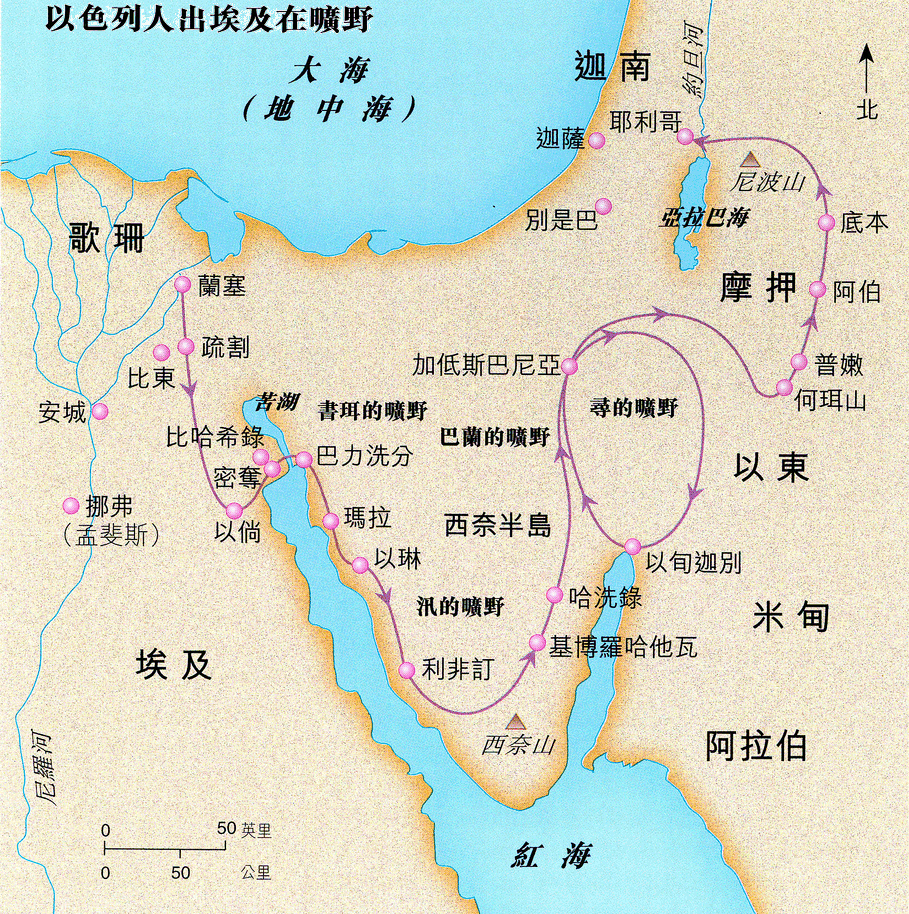
\includegraphics[width=0.38\textwidth]{AMoXiFigs/minshuji/Exodus}
\caption{出埃及地所行的路程}
\label{fig:chuaiji} 
\end{center}
\end{wrapfigure}
以色列人從蘭塞起行，安營在疏割。從疏割起行，安營在曠野邊的以倘。從以倘起行，轉到比哈希錄，是在巴力洗分對面，就在密奪安營。從比哈希錄對面起行，經過海中到了書珥曠野，又在伊坦的曠野走了三天的路程，就安營在瑪拉。從瑪拉起行，來到以琳，以琳有十二股水泉，七十棵棕樹，就在那裡安營。從以琳起行，安營在紅海邊。從紅海邊起行，安營在汛的曠野。從汛的曠野起行，安營在脫加。從脫加起行，安營在亞錄。從亞錄起行，安營在利非訂，在那裡百姓沒有水喝。從利非訂起行，安營在西奈的曠野。從西奈的曠野起行，安營在基博羅哈他瓦。從基博羅哈他瓦起行，安營在哈洗錄。從哈洗錄起行，安營在利提瑪。從利提瑪起行，安營在臨門帕烈。從臨門帕烈起行，安營在立拿。從立拿起行，安營在勒撒。從勒撒起行，安營在基希拉他。從基希拉他起行，安營在沙斐山。從沙斐山起行，安營在哈拉大。從哈拉大起行，安營在瑪吉希錄。從瑪吉希錄起行，安營在他哈。從他哈起行，安營在他拉。 從他拉起行，安營在密加。從密加起行，安營在哈摩拿。從哈摩拿起行，安營在摩西錄。從摩西錄起行，安營在比尼亞干。從比尼亞干起行，安營在曷哈及甲。從曷哈及甲起行，安營在約巴他。從約巴他起行，安營在阿博拿。從阿博拿起行，安營在以旬迦別。從以旬迦別起行，安營在尋的曠野，就是加低斯。從加低斯起行，安營在何珥山，以東地的邊界。

\subsubsection{出埃及地後四十年的行程 33:38-49}
以色列人出了埃及地後四十年，五月初一日，祭司亞倫遵著耶和華的吩咐上何珥山，就死在那裡。亞倫死在何珥山的時候年一百二十三歲。住在迦南南地的迦南人亞拉得王聽說以色列人來了。以色列人從何珥山起行，安營在撒摩拿。 42 從撒摩拿起行，安營在普嫩。 43 從普嫩起行，安營在阿伯。 44 從阿伯起行，安營在以耶亞巴琳，摩押的邊界。 45 從以耶亞巴琳起行，安營在底本迦得。 46 從底本迦得起行，安營在亞門低比拉太音。 47 從亞門低比拉太音起行，安營在尼波對面的亞巴琳山裡。 48 從亞巴琳山起行，安營在摩押平原約旦河邊，耶利哥對面。 49 他們在摩押平原沿約旦河邊安營，從伯耶施末直到亞伯什亭。

%\section{頒布律法 33:50-36 }


\subsubsection{過約旦河前的指示 33:50-56}
\noindent
1, 禁止拜当地人的偶像\\
耶和華在摩押平原約旦河邊，耶利哥對面，曉諭摩西說：「你吩咐以色列人說：你們過約旦河進迦南地的時候，就要從你們面前趕出那裡所有的居民，毀滅他們一切鏨成的石像和他們一切鑄成的偶像，又拆毀他們一切的丘壇。\\
2, 按照人口分地\\
你們要奪那地，住在其中，因我把那地賜給你們為業。你們要按家室拈鬮，承受那地。人多的，要把產業多分給他們；人少的，要把產業少分給他們。拈出何地給何人，就要歸何人。你們要按宗族的支派承受。\\
3, 全然趕出那地的居民\\
倘若你們不趕出那地的居民，所容留的居民就必做你們眼中的刺，肋下的荊棘，也必在你們所住的地上擾害你們。而且我素常有意怎樣待他們，也必照樣待你們。」

\subsection{九個半支派承受為業的邊界  34:1-29}
\subsubsection{南邊地界 34:1-5}
\begin{wraptable}{r}{12.5cm}
\vspace*{-8mm}
\centering
\begin{tabular}{|c|l|}\hline
\hline
位置  &地界劃分      \\ \hline\hline 
南角&\shortstack{尋的曠野、貼着以東的邊界、南界要從鹽海東頭起、\\繞到亞克拉濱坡的南邊、接連到尋、直通到加低斯巴尼亞的南邊、\\又通到哈薩亞達、接連到押們。從押們轉到埃及小河、直通到海為止。}\    \\ \hline
西邊&大海為界．\\  \hline
北界  &\shortstack{大海起、畫到何珥山．從何珥山畫到哈馬口、\\通到西達達．又通到西斐崙、直到哈薩以難}\ \\ \hline
東界&\shortstack{從哈薩以難畫到示番，從示番下到亞延東邊的利比拉、\\又要達到基尼烈湖的東邊。這界要下到約但河、通到鹽海}\ \\ \hline
\end{tabular}
\caption{九個半支派承受為業的邊界}
\end{wraptable}
耶和華曉諭摩西說：「你吩咐以色列人說：你們到了迦南地，就是歸你們為業的迦南四境之地：南角要從尋的曠野，貼著以東的邊界。南界要從鹽海東頭起，繞到亞克拉濱坡的南邊，接連到尋，直通到加低斯巴尼亞的南邊，又通到哈薩亞達，接連到押們，從押們轉到埃及小河，直通到海為止。

\subsubsection{西邊地界 34:6}
西邊要以大海為界。這就是你們的西界。

\subsubsection{北邊地界  34:7-9}
北界要從大海起，劃到何珥山，從何珥山劃到哈馬口，通到西達達，又通到西斐崙，直到哈薩以難。這要做你們的北界。

\subsubsection{東邊地界  34:10-12}
你們要從哈薩以難劃到示番為東界。這界要從示番下到亞延東邊的利比拉，又要達到基尼烈湖的東邊。這界要下到約旦河，通到鹽海為止。這四圍的邊界以內，要做你們的地。

\subsubsection{摩西吩咐以色列人九個半支派地界  34:13-15}
摩西吩咐以色列人說：「這地就是耶和華吩咐拈鬮給九個半支派承受為業的。因為魯本支派和迦得支派按著宗族受了產業，瑪拿西半個支派也受了產業。這兩個半支派已經在耶利哥對面，約旦河東，向日出之地受了產業。」

\newpage
\subsubsection{九個半支派支派分地的首領 34:16-29 }
\begin{wraptable}{r}{6.3cm}
\vspace*{-14mm}
\centering
\begin{tabular}{|c|c|c|}\hline\hline
支派  &父親名字 & 首領名字      \\ \hline\hline 
猶大&耶孚尼& 迦勒   \\ \hline
西緬& 亞米忽& 示母利\\  \hline
便雅憫& 基斯倫& 以利達 \\ \hline
但& 約利& 布基 \\ \hline
瑪拿西& 以弗& 漢聶\\ \hline
以法蓮&拾弗但&基母利\\ \hline
 西布倫&帕納&以利撒番\\ \hline
以薩迦&阿散&帕鐵\\ \hline
亞設&示羅米&亞希忽\\ \hline
拿弗他利&亞米忽&比大黑\\ \hline
\end{tabular}
\caption{九個半支派分地的首領}
\end{wraptable}
耶和華曉諭摩西說：「要給你們分地為業之人的名字是祭司以利亞撒和嫩的兒子約書亞。又要從每支派中選一個首領幫助他們。這些人的名字：猶大支派有耶孚尼的兒子迦勒；西緬支派有亞米忽的兒子示母利；便雅憫支派有基斯倫的兒子以利達；但支派有一個首領，約利的兒子布基；約瑟的子孫瑪拿西支派有一個首領，以弗的兒子漢聶；以法蓮支派有一個首領，拾弗但的兒子基母利；西布倫支派有一個首領，帕納的兒子以利撒番；以薩迦支派有一個首領，阿散的兒子帕鐵；亞設支派有一個首領，示羅米的兒子亞希忽；拿弗他利支派有一個首領，亞米忽的兒子比大黑。」 這些人就是耶和華所吩咐，在迦南地把產業分給以色列人的。

\subsection{利未支派 35}
\subsubsection{利未支派得城的原則 35:1-8 }
\begin{figure}[H]%{r}{0.5\textwidth} 
  \begin{center}
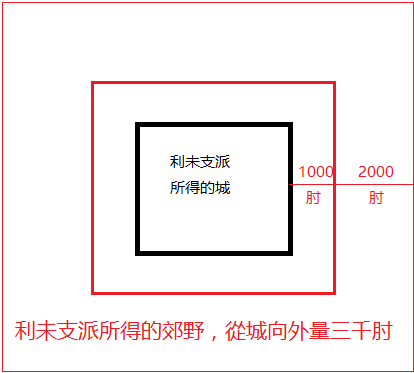
\includegraphics[width=.45\textwidth]{AMoXiFigs/minshuji/liwei}
\caption{利未支派得城的原則}
\end{center}
\end{figure} 
耶和華在摩押平原約旦河邊，耶利哥對面，曉諭摩西說：「你吩咐以色列人，要從所得為業的地中把些城給利未人居住，也要把這城四圍的郊野給利未人。這城邑要歸他們居住，城邑的郊野可以牧養他們的牛羊和各樣的牲畜，又可以安置他們的財物。你們給利未人的郊野，要從城根起，四圍往外量一千肘。另外東量二千肘、南量二千肘、西量二千肘、北量二千肘為邊界，城在當中。這要歸他們做城邑的郊野。你們給利未人的城邑，其中當有六座逃城，使誤殺人的可以逃到那裡，此外還要給他們四十二座城。你們要給利未人的城，共有四十八座，連城帶郊野都要給他們。以色列人所得的地業從中要把些城邑給利未人。人多的就多給，人少的就少給。各支派要按所承受為業之地把城邑給利未人。」


\subsubsection{設立逃城  35:9-15} 
耶和華曉諭摩西說：「你吩咐以色列人說：你們過約旦河，進了迦南地，就要分出幾座城，為你們做逃城，使誤殺人的可以逃到那裡。這些城可以做逃避報仇人的城，使誤殺人的不至於死，等他站在會眾面前聽審判。你們所分出來的城，要做六座逃城。在\textcolor{blue}{約旦河東}要分出三座城，在\textcolor{blue}{迦南地}也要分出三座城，都做逃城。這六座城要給\textcolor{blue}{以色列人}和他們\textcolor{blue}{中間的外人}，並\textcolor{blue}{寄居的}，作為逃城，使誤殺人的都可以逃到那裡。

\subsubsection{故殺人的逃城不能庇护 35:16-21} 
\begin{itemize} 
\itemsep-.35em
\item 若人\textcolor{blue}{用鐵器打人}，以致打死，他就是故殺人的，故殺人的必被治死。 
\item 若\textcolor{blue}{用可以打死人的石頭}打死了人，他就是故殺人的，故殺人的必被治死。 
\item 若\textcolor{blue}{用可以打死人的木器}打死了人，他就是故殺人的，故殺人的必被治死。報血仇的必親自殺那故殺人的，一遇見就殺他。 
\item 人若因\textcolor{blue}{怨恨把人推倒}，或是\textcolor{blue}{埋伏往人身上扔物}以至於死
\item 或是\textcolor{blue}{因仇恨用手打人}以至於死，那打人的必被治死。他是故殺人的，報血仇的一遇見就殺他。
\end{itemize}

\subsubsection{逃城的庇护原则  35:22-28} 
倘若人沒有仇恨，忽然將人推倒，或是沒有埋伏把物扔在人身上，或是沒有看見的時候用可以打死人的石頭扔在人身上，以至於死，本來與他無仇，也無意害他，會眾就要照典章，在打死人的和報血仇的中間審判。會眾要救這誤殺人的脫離報血仇人的手，也要使他歸入逃城。\\
他要住在其中，直等到受聖膏的大祭司死了。但誤殺人的，無論什麼時候，若出了逃城的境外，報血仇的在逃城境外遇見他，將他殺了，報血仇的就沒有流血之罪。 因為誤殺人的該住在逃城裡，等到大祭司死了。大祭司死了以後，誤殺人的才可以回到他所得為業之地。

\subsubsection{故殺人犯死罪的必被治死  35:29-34} 
「這在你們一切的住處，要做你們世世代代的律例、典章。無論誰故殺人，要憑幾個見證人的口把那故殺人的殺了，只是不可憑一個見證的口叫人死。故殺人，犯死罪的，你們\textcolor{red}{不可收贖價代替他的命}，他必被治死。那逃到逃城的人，你們不可為他收贖價，使他在大祭司未死以先再來住在本地。這樣，你們就不汙穢所住之地，因為血是汙穢地的。若有在地上流人血的，非流那殺人者的血，那地就不得潔淨(贖)。你們不可玷汙所住之地，就是我住在其中之地，因為我耶和華住在以色列人中間。」
 	
 	
\subsection{女子承地為業的條例 36 }
\subsubsection{瑪拿西族長在摩西和首領面前的诉求 36:1-4}
約瑟的後裔，瑪拿西的孫子、瑪吉的兒子基列，他子孫中的諸族長來到摩西和做首領的以色列人族長面前，說：「耶和華曾吩咐我主拈鬮分地給以色列人為業，我主也受了耶和華的吩咐將我們兄弟西羅非哈的產業分給他的眾女兒。她們若嫁以色列別支派的人，就必將我們祖宗所遺留的產業加在她們丈夫支派的產業中。這樣，我們拈鬮所得的產業就要減少了。到了以色列人的禧年，這女兒的產業就必加在她們丈夫支派的產業上。這樣，我們祖宗支派的產業就減少了。」
 
\subsubsection{得業女子必嫁同宗支派的人 36:5-9}
摩西照耶和華的話吩咐以色列人說：「約瑟支派的人說得有理。論到西羅非哈的眾女兒，耶和華這樣吩咐說：她們可以隨意嫁人，只是要嫁同宗支派的人。這樣，以色列人的產業就不從這支派歸到那支派，因為以色列人要各守各祖宗支派的產業。凡在以色列支派中得了產業的女子，必做同宗支派人的妻，好叫以色列人各自承受他祖宗的產業。這樣，他們的產業就不從這支派歸到那支派，因為以色列支派的人要各守各的產業。」

\subsubsection{西羅非哈的五女都嫁入瑪拿西子孫 36:10-12}
耶和華怎樣吩咐摩西，西羅非哈的眾女兒就怎樣行。西羅非哈的女兒瑪拉、得撒、曷拉、密迦、挪阿都嫁了她們伯叔的兒子。她們嫁入約瑟兒子瑪拿西子孫的族中，她們的產業仍留在同宗支派中。這是耶和華在摩押平原約旦河邊，耶利哥對面藉著摩西所吩咐以色列人的命令、典章。


